
%%%%%%%%%%%%%%%%%%%%%%%%%%%%%%%%%%%%%%%%%%%%%%%%%%
%%                                              %%
%%           Modelo para criação de             %%
%%            trabalhos acadêmicos              %%
%%                                              %%
%%%%%%%%%%%%%%%%%%%%%%%%%%%%%%%%%%%%%%%%%%%%%%%%%%

\documentclass[
    a4paper,        % papel A4
    12pt,           % fonte 12
    oneside,        % impressão em apenas uma face do papel
    %article,        % formato para artigos
    english,        % hifenizações em inglês
    brazil,         % idioma padrão do documento
]{abntex2}


% inclusão dos pacotes usados

%%%%%%%%%%%%%%%%%%%%%%%%%%%%%%%%%%%%%%%%%%%%%%%%%%
%%                                              %%
%%          Importação de pacotes               %%
%%                                              %%
%%%%%%%%%%%%%%%%%%%%%%%%%%%%%%%%%%%%%%%%%%%%%%%%%%

% Acrônimos (Siglas e Abreviaturas)
\usepackage{acronym}

% Pacote para o desenvolvimento de algoritmos e codificação utf8
\usepackage[portuguese,lined,boxed,ruled]{algorithm2e}
\usepackage{algorithmic}

% Fontes e símbolos matemáticos
\usepackage{amsfonts, amsmath, amssymb}

\usepackage[brazil]{babel}

\usepackage{booktabs}


% Manutenção das legendas em imagens (fonte pequena, 10pt)
\usepackage[font=small]{caption}

% Manutenção da marcação em listas (enumerator)
\usepackage{enumitem}

% Codificação da fonte em 8 bits
\usepackage[T1]{fontenc}

% Inserir figuras
\usepackage{graphicx}

% Dimensões do documento
\usepackage[left=3.0cm, right=2.0cm, top=3.0cm, bottom=2.0cm]{geometry}

% Glossário
\usepackage[nonumberlist,style=index]{glossaries}

% Hifenização das palavras 
\usepackage{hyphenat}

% Índice
\usepackage{imakeidx}


% Identar do primeiro parágrafo de cada seção
\usepackage{indentfirst}

% Acentuação direta
\usepackage[utf8]{inputenc}

% para melhorias de justificação
\usepackage{microtype}

% Mescla de células em tabelas
\usepackage{multirow}

\usepackage{placeins}

% Rotacionar elementos
\usepackage{rotating}

% Manutenção do espaçamento entre linhas
\usepackage{setspace}

% Texto em Times New Roman
\usepackage{times}

%\usepackage{tocloft}

%%%%%%%%%%%%%%%%%%%%%%%%%%%%
%% Pacotes com Hierarquia %%
%%%%%%%%%%%%%%%%%%%%%%%%%%%%

\usepackage[brazilian, hyperpageref]{backref}	 % Paginas com as citações na bibl

% Referências
\usepackage[alf, bibjustif, abnt-etal-list=0, abnt-etal-text=it]{abntex2cite}



% ---
% Configurações do pacote backref
% Usado sem a opção hyperpageref de backref
\renewcommand{\backrefpagesname}{Citado na(s) página(s):~}
% Texto padrão antes do número das páginas
\renewcommand{\backref}{}
% Define os textos da citação
\renewcommand*{\backrefalt}[4]{
	\ifcase #1 %
		Nenhuma citação no texto.%
	\or
		Citado na página #2.%
	\else
		Citado #3 vezes nas páginas #2.%
	\fi}%
% ---
% inclusão das informações do documento e métodos criados e alterados
%%%%%%%%%%%%%%%%%%%%%%%%%%%%%%%%%%%%%%%%%%%%%%%%%%
%%                                              %%
%%        Comandos usados no documento          %%
%%                                              %%
%%%%%%%%%%%%%%%%%%%%%%%%%%%%%%%%%%%%%%%%%%%%%%%%%%
% Capa e Folha de Rosto
\renewcommand{\imprimircapa}{
%%%%%%%%%%%%%%%%%%%%%%%%%%%%%%%%%%%%%%%%%%%%%%%%%%
%%                                              %%
%%              Início da Capa                  %%
%%                                              %%
%%%%%%%%%%%%%%%%%%%%%%%%%%%%%%%%%%%%%%%%%%%%%%%%%%

\thispagestyle{empty}

\begin{figure}
    \centering
    \includegraphics[]{lib/Logoufrn.jpg}
\end{figure}

\begin{center}
    \large{\imprimirinstituicao}
    
    \vspace{\stretch{2}}
    
    \large{\MakeUppercase{\imprimirtitulo: \imprimirsubtitulo}}
    
    \vspace{\stretch{2}}
    
    \large{\MakeUppercase{\textbf{\imprimirautor}}}
    
    \vspace{\stretch{3}}
    
    \large{\imprimirlocal} \\
    \large{\imprimirdata}
\end{center}

\newpage
%%%%%%%%%%%%%%%%%%%%%%%%%%%%%%%%%%%%%%%%%%%%%%%%%%
%%                                              %%
%%                  Fim da Capa                 %%
%%                                              %%
%%%%%%%%%%%%%%%%%%%%%%%%%%%%%%%%%%%%%%%%%%%%%%%%%%}
\renewcommand{\imprimirfolhaderosto}{
%%%%%%%%%%%%%%%%%%%%%%%%%%%%%%%%%%%%%%%%%%%%%%%%%%
%%                                              %%
%%          Início da Folha de Rosto            %%
%%                                              %%
%%%%%%%%%%%%%%%%%%%%%%%%%%%%%%%%%%%%%%%%%%%%%%%%%%

\thispagestyle{empty}

\begin{center}
    % Imprime o nome do autor depois coloca um espaçamento vertical de 3 vezes o espaçamento existente entre os textos
    \large{\MakeUppercase{\textbf{\imprimirautor}}}
    \vspace*{\stretch{3}}
    
    % Imprime o título do trabalho depois coloca um espaçamento vertical padrão dentre os textos da página
    \large{\MakeUppercase{\imprimirtitulo: \imprimirsubtitulo}}
    \vspace{\stretch{1}}
    
    % Inicia a mini página alinhada horizontalmente com o comprimento da linha sendo a metade da mesma imprimindo o preâmbulo, o orientador do trabalho e o co-orientador (se houver). Após a mini página o espaçamento vertical
    \hfill
    \begin{minipage}{.5\linewidth}
        \small\imprimirpreambulo
        \\ [0.6cm]
        \small \imprimirorientadorRotulo \imprimirorientador.\\
        \small \imprimircoorientadorRotulo
        \small \imprimircoorientador.
    \end{minipage}
    \vspace{\stretch{1}}
    
    % Imprime local e data do trabalho
    \large{\imprimirlocal}\\
    \large{\imprimirdata}
\end{center}

\newpage
%%%%%%%%%%%%%%%%%%%%%%%%%%%%%%%%%%%%%%%%%%%%%%%%%%
%%                                              %%
%%            Fim da Folha de Rosto             %%
%%                                              %%
%%%%%%%%%%%%%%%%%%%%%%%%%%%%%%%%%%%%%%%%%%%%%%%%%%
}

% subtítulo
\providecommand{\imprimirsubtitulo}{}
\newcommand{\subtitulo}[1]{\renewcommand{\imprimirsubtitulo}{#1}}

% criar fonte em imagens, tabelas e quadros
\newcommand{\source}[1]{\legend{\textbf{Fonte:} {#1}}}    

%%%%%%%%%%%%%%%%%%%%%%%%%%%%%%%%%%%%%%%%%%%%%%%%%%
%%                                              %%
%%          Informações do documento            %%
%%                                              %%
%%%%%%%%%%%%%%%%%%%%%%%%%%%%%%%%%%%%%%%%%%%%%%%%%%

\titulo{\textbf{Aprendizado semissupervisionado aplicado à classificação}}

\subtitulo{um estudo de caso com o \textit{FlexCon\hyp{C}} para análise da variação do limiar}

\tipotrabalho{Monografia (bacharel em Sistema de Informação)}

\autor{Arthur Costa Gorg\^{o}nio}

\orientador{MSc. Amarildo Jeiele Ferreira de Lucena}     % nível acadêmico + nome

\coorientador{MSc. Karliane Medeiros Ovidio Vale}

%%%%%%%%%%%%%%%%%%%%%%%%%%%%
%% Pacotes com Hierarquia %%
%%%%%%%%%%%%%%%%%%%%%%%%%%%%

% Rótulo do orientador
\renewcommand{\imprimirorientadorRotulo}{Orientador(a): }
\renewcommand{\imprimircoorientadorRotulo}{Co-orientador(a): }

\local{Caicó - RN}

\data{\the\year}

\instituicao{
    UNIVERSIDADE FEDERAL DO RIO GRANDE DO NORTE \\
    CENTRO DE ENSINO SUPERIOR DO SERIDÓ \\
    DEPARTAMENTO DE COMPUTAÇÃO E TECNOLOGIA \\
    BACHARELADO EM SISTEMAS DE INFORMAÇÃO
}

%% Se for TCC II acrescente mais um I
\preambulo{\textbf{Trabalho de Conclusão de Curso II}, apresentado ao Curso de Bacharelado em Sistemas de Informação da Universidade Federal do Rio Grande do Norte, como parte dos requisitos para obtenção do título de Bacharel em Sistemas de Informação.}

%%%%%%%%%%%%%%%%%%%%%%%%%%%%%%%%%%
%%                              %%
%%          Numeração           %%
%%                              %%
%%%%%%%%%%%%%%%%%%%%%%%%%%%%%%%%%%
\counterwithout{equation}{chapter}

%%%%%%%%%%%%%%%%%%%%%%%%%%%%%%%%%%
%%                              %%
%%            Quadros           %%
%%                              %%
%%%%%%%%%%%%%%%%%%%%%%%%%%%%%%%%%%
\newcommand{\quadroname}{Quadro}

\newfloat[chapter]{quadro}{loq}{\quadroname}
\newlistof{listofquadros}{loq}{\listofquadrosname}
\newlistentry{quadro}{loq}{0}

% configurações para atender às regras da ABNT
%\setfloatadjustment{quadro}{\centering}
\counterwithout{quadro}{chapter}
\renewcommand{\cftquadroname}{\quadroname\space} 
\renewcommand*{\cftquadroaftersnum}{\hfill--\hfill}

%%%%%%%%%%%%%%%%%%%%%%%%%%%%%%%%%%%%%%%%%%%%%%%%%%
%%                                              %%
%%   Configurações de aparência do PDF final    %%
%%                                              %%
%%%%%%%%%%%%%%%%%%%%%%%%%%%%%%%%%%%%%%%%%%%%%%%%%%
%%%%%%%%%%%%%%%%%%%%%%%%%%%%%%%%%%
%%                              %%
%%         Indentação           %%
%%                              %%
%%%%%%%%%%%%%%%%%%%%%%%%%%%%%%%%%%

% O tamanho do parágrafo é dado por:
\setlength{\parindent}{1.5cm}

% Controle do espaçamento entre um parágrafo e outro:
\setlength{\parskip}{0.2cm}  % tente também \onelineskip

%%%%%%%%%%%%%%%%%%%%%%%%%%%%%%%%%%
%%                              %%
%%      Informações do PDF      %%
%%                              %%
%%%%%%%%%%%%%%%%%%%%%%%%%%%%%%%%%%
\makeatletter
\hypersetup{
	pdftitle={\@title}, 
	pdfauthor={\@author},
    pdfsubject={\imprimirpreambulo},
    pdfcreator={LaTeX with abnTeX2},
	pdfkeywords={abnt}{latex}{abntex}{abntex2}{trabalho acadêmico}, 
%   false: boxed links; true: colored links
	colorlinks=true,
% 	color of internal links
    linkcolor=blue,
%   color of links to bibliography
    citecolor=blue,
%   color of file links
    filecolor=magenta,
	urlcolor=blue,
	bookmarksdepth=4
}
\makeatother


% Algoritmos
% \TitleOfAlgo{title}
% \floatname{algorithm}{Algoritmo}%Algoritmo
% \renewcommand{\listalgorithmname}{LISTA DE ALGORITMOS}
\renewcommand{\algorithmcfname}{Pseudocódigo}
\renewcommand{\algorithmicindent}{3.0em}
\renewcommand{\algorithmicrequire}{\textbf{entrada}}
\renewcommand{\algorithmicensure}{\textbf{garanta}}
\renewcommand{\algorithmicreturn}{\textbf{retorne}}
\renewcommand{\algorithmicor}{\textbf{ou}}
\renewcommand{\algorithmicand}{\textbf{e}}
\renewcommand{\algorithmicend}{\textbf{fim}}
\renewcommand{\algorithmicif}{\textbf{se}}
\renewcommand{\algorithmicelse}{\textbf{sen\~ao}}
\renewcommand{\algorithmicthen}{\textbf{ent\~ao}}
\renewcommand{\algorithmicfor}{\textbf{para}}
\renewcommand{\algorithmicforall}{\textbf{para cada}}
\renewcommand{\algorithmicrepeat}{\textbf{repita}}
\renewcommand{\algorithmicuntil}{\textbf{até que}}
\renewcommand{\algorithmicwhile}{\textbf{enquanto}}
\renewcommand{\algorithmicdo}{\textbf{fa\c{c}a}}

%
%%%%%%%%%%%%%%%%%%%%%%%%%%%%%%%%%%%%%
%%      Entradas do glossário      %%
%%%%%%%%%%%%%%%%%%%%%%%%%%%%%%%%%%%%%

% Aqui devem estar todas as entradas de seu glossário

\newglossaryentry{Entrada1}{
    name={nome da entrada1},
    description={descrição da entrada1}
}
%  .
%  .
%  .

\newglossaryentry{EntradaN}{
    name={nome da entradaN},
    description={descrição da entradaN}
}

% Cria o glossário
% \makeglossaries

%\makeindex

\begin{document}
    \mainmatter
    %%%%%%%%%%%%%%%%%%%%%%%%%%%%%%%%%%
    %%                              %%
    %%    Elementos Pré-textuais    %%
    %%                              %%
    %%%%%%%%%%%%%%%%%%%%%%%%%%%%%%%%%%
    \pretextual

    %espaçamento de 1.0
    \begin{SingleSpace}
        % Elemento Obrigatório para TCC I e II
        \imprimircapa

        % paginação em números
        \pagenumbering{arabic}

        % Elemento Obrigatório Para TCC I e II
        \imprimirfolhaderosto

    \end{SingleSpace}

    % Elemento Obrigatório TCC II
    %\begin{fichacatalografica}
	\sffamily
	\vspace*{\fill}					% Posição vertical
	\begin{center}					% Minipage Centralizado
	\fbox{\begin{minipage}[c][8cm]{13.5cm}		% Largura
	\small
	\imprimirautor
	%Sobrenome, Nome do autor
	
	\hspace{0.5cm} \imprimirtitulo  / \imprimirautor. --
	\imprimirlocal, \imprimirdata-
	
	\hspace{0.5cm} \thelastpage f. : il.\\
	
	\hspace{0.5cm} \imprimirorientadorRotulo~\imprimirorientador\\
	
	\hspace{0.5cm}
	{\imprimirtipotrabalho~--~\imprimirinstituicao,
	\imprimirdata.}\\
	
	\hspace{0.5cm}
		1. Palavra-chave1.
		2. Palavra-chave2.
		2. Palavra-chave3.
		I. Orientador. %Referência do orientador
		II. Universidade xxx.
		III. Faculdade de xxx.
		IV. Título 			
	\end{minipage}}
	\end{center}
\end{fichacatalografica}

\newpage

    % Elemento Opcional para TCC I e II
    %\begin{errata}
    texto.
\end{errata} 


    % Elemento Obrigatório para TCC II
    %\begin{folhadeaprovacao}

    \begin{center}
        {\ABNTEXchapterfont\large\imprimirautor}

        \vspace*{\fill}\vspace*{\fill}
        
        \begin{center}
            \ABNTEXchapterfont\bfseries\Large\imprimirtitulo
        \end{center}
        
        \vspace*{\fill}
            
        \hspace{.45\textwidth}
        \begin{minipage}{.5\textwidth}
            \imprimirpreambulo
        \end{minipage}%
            \vspace*{\fill}
        
       \textbf{\imprimirlocal}, 16 de novembro de \imprimirdata
   \end{center}

   \assinatura{\textbf{\imprimirorientador} \\ Orientador} 
   \assinatura{\textbf{Professor} \\ Co-Orientador}
   \assinatura{\textbf{Professor} \\ Examinador(a) 1}
   \assinatura{\textbf{Professor} \\ Examinador(a) 2}
   %\assinatura{\textbf{Professor} \\ Examinador(a) 3}
   %\assinatura{\textbf{Professor} \\ Examinador(a) 4}
      
   \begin{center}
    \vspace*{0.5cm}
    {\large\imprimirlocal}
    \par
    {\large\imprimirdata}
    \vspace*{1cm}
  \end{center}
  
\end{folhadeaprovacao}

    % Elemento Opcional para TCC II
    %\begin{dedicatoria}
    \vspace*{\fill}
    \centering
    \noindent
    \textit{Eu dedico esse trabalho à ...}
    \vspace*{\fill}
\end{dedicatoria}

    % Elemento Opcional para TCC II
    %\begin{agradecimentos}
    Agradeço às minhas pernas por me sustentarem, aos meus braços por sempre estarem ao meu lado, e aos meus dedos, pois sempre pude contar com eles.
\end{agradecimentos}

    % Elemento Opcional para TCC II
    %\begin{epigrafe}
    \vspace*{\fill}
	\begin{flushright}
		\textit{``Não vos amoldeis às estruturas deste mundo, \\
		mas transformai-vos pela renovação da mente, \\
		a fim de distinguir qual é a vontade de Deus: \\
		o que é bom, o que Lhe é agradável, o que é perfeito.\\
		(Bíblia Sagrada, Romanos 12, 2)}
	\end{flushright}
\end{epigrafe}

    % Elemento Obrigatório para TCC II
    
%%%%%%%%%%%%%%%%%%%%%%%%%%%%
%%                        %%
%%         Resumo         %%
%%                        %%
%%%%%%%%%%%%%%%%%%%%%%%%%%%%

\begin{resumo}
   \noindent
%Escreva aqui.


    \textbf{Palavras-chave}: 
\end{resumo}

%%%%%%%%%%%%%%%%%%%%%%%%%%%%
%%                        %%
%%        Abstract        %%
%%                        %%
%%%%%%%%%%%%%%%%%%%%%%%%%%%%

\begin{resumo}[Abstract]
    \noindent
%Write here

    
    \textbf{Keywords}:
\end{resumo}



    % Figuras, Quadros, Tabelas e Sumário.
    % Algumas Obrigatórias outras não TCC I
    
%%%%%%%%%%%%%%%%%%%%%%%%%%%%%%
%%          Listas          %%
%%%%%%%%%%%%%%%%%%%%%%%%%%%%%%

%%%%%%%%%%%%%%%%%%%%%%%%%%%%%%%%%%%%%%%%%%
%%                                      %%
%%              Figuras                 %%
%%                                      %%
%%%%%%%%%%%%%%%%%%%%%%%%%%%%%%%%%%%%%%%%%%
\thispagestyle{empty}

\renewcommand{\listfigurename}{\normalsize{\textbf{LISTA DE FIGURAS}}}

\listoffigures*
\newpage

%%%%%%%%%%%%%%%%%%%%%%%%%%%%%%%%%%%%%%%%%%
%%                                      %%
%%              Quadros                 %%
%%                                      %%
%%%%%%%%%%%%%%%%%%%%%%%%%%%%%%%%%%%%%%%%%%
\thispagestyle{empty}

\newcommand{\listofquadrosname}{\normalsize{\textbf{LISTA DE QUADROS}}}

\listofquadros*
\newpage

%%%%%%%%%%%%%%%%%%%%%%%%%%%%%%%%%%%%%%%%%%
%%                                      %%
%%              Tabelas                 %%
%%                                      %%
%%%%%%%%%%%%%%%%%%%%%%%%%%%%%%%%%%%%%%%%%%
\thispagestyle{empty}

\renewcommand{\listtablename}{\normalsize{\textbf{LISTA DE TABELAS}}}

\listoftables*
\newpage


%%%%%%%%%%%%%%%%%%%%%%%%%%%%%%%%%%%%%%%%%%
%%                                      %%
%%              Siglas                  %%
%%                                      %%
%%%%%%%%%%%%%%%%%%%%%%%%%%%%%%%%%%%%%%%%%%
\thispagestyle{empty}

\chapter*{\normalsize{\textbf{LISTA DE ABREVIATURAS E SIGLAS}}}

\begin{acronym}[]
    \acro{am}[AM]{Aprendizado de Máquina}
    \acro{anova}[ANOVA]{\textit{ANalysis Of VAriance}}
    \acro{flexcon}[FlexCon\hyp{C}]{\textit{Flexible Confidence with Classifier}}
    \acro{knn}[\textit{k}\hyp{NN}]{\textit{\textit{k}\hyp{Nearest} Neighbors}}
    \acro{irep}[IREP]{\textit{Incremental Reduced Error Pruning}}
    \acro{rpart}[rpart]{\textit{Recursive Partitioning and Regression Trees}}
    \acro{rep}[REP]{\textit{Reduced Error Pruning}}
    \acro{ripper}[\textsc{ripper}]{\textit{Repeated Incremental Pruning to Produce Error Reduction}}
    \acro{ssl}[SSL]{\textit{Semi\hyp{Supervised} Learning}}
\end{acronym}

\newpage

%%%%%%%%%%%%%%%%%%%%%%%%%%%%%%%%%%%%%%%%%%
%%                                      %%
%%              Símbolos                %%
%%                                      %%
%%%%%%%%%%%%%%%%%%%%%%%%%%%%%%%%%%%%%%%%%%
\renewcommand{\listadesimbolosname}{\normalsize{\textbf{LISTA DE SÍMBOLOS}}}

\begin{simbolos}
    \item[$D$] Conjunto dos dados, incluindo dados rotulados e não rotulados
    \item[$L$] Conjunto dos dados rotulados
    \item[$U$] Conjunto dos dados não rotulados
    \item[$X$] Conjunto dos exemplos
    \item[$Y$] Conjunto das classes
    \item[$f$] Classificador
    \item[$x_i$] \textit{i}\hyp{ésimo} exemplo
    \item[$y_i$] \textit{i}\hyp{ésima} classe
    \item[$(x_i, y_i)$] Par do \textit{i}\hyp{ésimo} exemplo com sua respectiva classe
\end{simbolos}

%%%%%%%%%%%%%%%%%%%%%%%%%%%%%%%%%%%%%%%%%%
%%                                      %%
%%           Algoritmos                 %%
%%                                      %%
%%%%%%%%%%%%%%%%%%%%%%%%%%%%%%%%%%%%%%%%%%
\thispagestyle{empty}

\renewcommand{\listalgorithmcfname}{\normalsize{\textbf{LISTA DE PSEUDOCÓDIGOS}}}

\listofalgorithms

\newpage

%%%%%%%%%%%%%%%%%%%%%%%%%%%%%%%
%%          Sumário          %%
%%%%%%%%%%%%%%%%%%%%%%%%%%%%%%%


\renewcommand{\contentsname}{\normalsize{\textbf{SUMÁRIO}}}
\tableofcontents*
\newpage


    %%%%%%%%%%%%%%%%%%%%%%%%%%%%%%%%%%
    %%                              %%
    %%      Elementos Textuais      %%
    %%                              %%
    %%%%%%%%%%%%%%%%%%%%%%%%%%%%%%%%%%
    % Esse comando define as estruturas a seguir como elementos textuais
    \textual

    % Elemento Obrigatório para TCC I e II
    
%%%%%%%%%%%%%%%%%%%%%%%%%%%%%%%%%%%%%%
%%            Introdução            %%
%%%%%%%%%%%%%%%%%%%%%%%%%%%%%%%%%%%%%%

\chapter{Introdução}
    \label{cha:intro}
    Por um tempo, o computador foi utilizado prioritariamente para efetuar cálculos e retornar resultados. A evolução da tecnologia proporcionou facilidades para a humanidade, incluindo a popularização dos meios de informação e comunicação, melhoria da qualidade de vida e a automatização nos processos. Diante deste cenário, ocorreram avanços na coleta, armazenamento e processamento de dados, além do desenvolvimento de algoritmos capazes de formular modelos e aprender padrões. As máquinas tornaram\hyp{se} estratégicas no auxílio ao processo de tomada de decisão, pois a sua capacidade de processar dados é significativamente maior, comparada a dos humanos.
    
    \section{Contextualização e Problema}
    \label{subsec:contextualizacao-problema}
    
    % Aprendizado de Máquina
    % Aprendizado Semi-Supervisionado
        % Self-Training
    % classificadors de Aprendizagem (classificadores)
    % Limiar de taxa fixa
    
    \citeonline{mitchell1997machine} afirma que um programa de computador aprende com a experiência $E$, em relação a alguma classe de tarefas $T$ e com o seu desempenho mensurado por $P$, se seu desempenho nas tarefas $T$, medidos por $P$, melhoram com a experiência $E$. Isto é, quando a máquina realiza uma escolha, tendo como base um histórico obtido pela mesma, essa decisão é definida como \ac{am}.

    % O \ac{am} apresenta\hyp{se} como uma possível solução para análise de grandes volumes de dados, pois quando tais análises são desenvolvida por seres humanos, possuem alguns empecilhos, dentre eles: a incapacidade do processamento humano sobre grandes volumes de dados e a necessidade de especialistas sobre o domínio dos dados para serem bem analisados. Por sua vez, uma máquina que possua a característica de aprendizado pode realizar esse processo de análise mais rápida e com um custo reduzido.
    O \ac{am} apresenta\hyp{se} como uma possível solução para a análise de grandes volumes de dados, uma vez que estas análises possuem algumas dificuldades quando desenvolvidas por seres humanos. Grandes volumes de dados demandam muito tempo para humanos processarem, além de serem necessários especialistas sobre o domínio dos dados para serem bem analisados. Por sua vez, uma máquina que possua a característica de aprendizado pode realizar esse processo de análise mais rápida e com um custo reduzido. Assim, surgiu a necessidade de desenvolver algoritmos capazes de aprender padrões e realizar tais tarefas.
    
    % dentre eles: i) o custo elevado; ii) necessidade de especialistas iii) risco da realização de análises subjetivas; iv) gasto de tempo em grandes volumes de dados. P
    
    % pode desenvolver a capacidade de extração de informações e realizar tais tarefas com um custo reduzido.
    
    A literatura descreve que o \ac{am} possui tarefas de classificação, agrupamento (\textit{clustering}) e regressão. \citeonline{alpaydin2004introduction} e \citeonline{mohri2012foundations} descrevem como:
    \begin{enumerate}[label=\roman*.]
        \item Classificação {--} Cada objeto é associado a um rótulo que representa uma das classes existentes, a partir de instâncias cujo rótulo seja conhecido;
        \item Agrupamento (\textit{clustering}) {--} Os objetos são agrupados de acordo com suas características, de forma que um objeto não pertença simultaneamente a mais de um agrupamento;
        \item Regressão {--} A partir de funções matemáticas, busca\hyp{se} encontrar relações algébricas entre atributos;
    \end{enumerate}
    
    \citeonline{chapelle2006semi} descrevem que no \ac{am} tradicionalmente existem dois tipos de tarefas, o aprendizado supervisionado e o aprendizado não supervisionado. O aprendizado supervisionado faz uso de classificação ou regressão, enquanto o aprendizado não supervisionado faz uso de agrupamentos (\textit{clusterings}).
    
    
    A técnica de \textit{clustering} é capaz de realizar uma separação dos objetos de acordo com suas similaridades baseando\hyp{se} em um conjunto de características. Essa técnica pode ser utilizada quando não existe a necessidade de identificar a qual classe um determinado objeto pertence. Na classificação de dados, os algoritmos auxiliam no processo de encontrar padrões em grandes quantidades de dados. Essa técnica é utilizada quando é desejado treinar a máquina para identificar a categoria a qual pertence um determinado objeto.
    
    O treinamento é uma etapa decisiva na obtenção de um modelo capaz de classificar corretamente os objetos com base em suas características. Nesta etapa, o algoritmo de classificação é aplicado sobre um conjunto de dados com a finalidade de gerar um classificador. A partir deste, é possível desempenhar a tarefa de classificação sobre novos conjuntos de dados.
    
    Um dos desafios do \ac{am} está em como realizar esse treinamento, pois nem sempre as bases de dados possuem objetos suficientes para realizá\hyp{lo} pelas formas tradicionais. Por isso, uma área tem ganhado muita atenção dos pesquisadores, o Aprendizado Semissupervisionado (\ac{ssl}) que, a partir de uma pequena parcela de objetos classificados, consegue atribuir as classes ao restante. Ou seja, a necessidade de possuir um grande conjunto de dados com o seu devido rótulo deixa de ser prioridade, pois o conjunto de dados classificado passa a ser maior ao fim de cada iteração do algoritmo.
    
    % algoritmos SSL pegam n exemplos por iteração
    % uso de limiares
    % taxa de controle do limiar
    %
    %
    
    Os algoritmos do \ac{ssl} são capazes de realizar o treinamento a partir de um conjunto pequeno de instâncias inicialmente rotuladas e normalmente classificam \textit{n} instâncias por iteração. Há variações destes algoritmos que fazem uso de limiares (confiança mínima) com a intenção de inserir no conjunto dos dados rotulados somente as instâncias que possuem a confiança atribuída pelo classificador, maior que o limiar. Isto é, o limiar é um fator de inclusão que torna variável o número de instâncias que são incluídas por iteração, pois só são selecionadas as instâncias com alto valor de confiança.
    
    %O uso do limiar fixo possui uma desvantagem, pode resultar na não classificação de todo o conjunto de dados. Existem diversas maneiras de resolver essa situação, dentre elas, utilizar uma taxa de controle, que auxilie na variação do limiar, ora aumentando, ora diminuindo esse valor, de forma a permitir a inclusão de novas instâncias.
    
    O uso do limiar fixo pode resultar na não classificação de todo o conjunto de dados. Sendo assim, uma das formas de resolver esse problema é utilizando uma taxa de controle, que auxilie na variação do limiar, ora aumentando, ora diminuindo esse valor, de forma a permitir a inclusão de novas instâncias.
    
    % Os algoritmos que fazem uso de uma taxa de controle para a variação do limiar normalmente a fixam, qual o impacto na classificação de dados caso essa taxa seja para a cada iteração? Então, este trabalho pretende fazer uso de um taxa variável para tentar melhorar métodos já propostos em outros estudos.
    
    \citeonline{vale2018selftraining} apresenta o método \ac{flexcon}, que faz uso do limiar e de um fator (taxa de variação) que altera\hyp{o} de maneira mais lenta. Esse método possui duas técnicas de implementação são elas: \textit{FlexCon\hyp{C1}} e \textit{FlexCon\hyp{C2}}. O \textit{FlexCon\hyp{C1}} faz uma comparação entre a predição da iteração atual com a predição da primeira iteração. O \textit{FlexCon\hyp{C2}} compara a predição atual com a predição de um classificador supervisionado que é treinado com o conjunto de instâncias que estão inicialmente rotuladas. Este trabalho pretende analisar o impacto na classificação dos dados quando a taxa de variação do limiar é manipulada.
    
    % \citeonline{vale2018selftraining} apresenta o algoritmo \ac{flexcon}, que faz uso do limiar e de um fator (taxa de variação) que altera\hyp{o} de maneira mais lenta. Esse algoritmo possui duas variações são elas: \textit{FlexCon\hyp{C1}} e \textit{FlexCon\hyp{C2}}. O \textit{FlexCon\hyp{C1}} faz uma comparação entre a predição da iteração atual com a predição da primeira iteração. O \textit{FlexCon\hyp{C2}} compara a predição atual com a predição de um classificador supervisionado que é treinado com o conjunto de instâncias que estão inicialmente rotuladas. Neste trabalho foi analisado o impacto na classificação dos dados quando a taxa de variação do limiar é alterada.
    \section{Objetivos}
    \label{sec:objetivos}

    Neste tópico são apresentados os objetivos desta pesquisa, divididos em geral e específicos.

    \subsection{Objetivo Geral}
        \label{subsec:objetivo-geral}
        % Este trabalho tem por objetivo aplicar as variações do algoritmo \textit{Self\hyp{Training}} sendo elas \textit{FlexConf\hyp{C1}} e \textit{FlexConf\hyp{C2}} manipulando a variação da taxa de confiança e avalia\hyp{las}.

        % Este trabalho tem por objetivo analisar dois dos métodos propostos em~\citeauthor{vale2018selftraining} e manipular a taxa de variação do limiar de tais métodos.

        %Este trabalho tem por objetivo analisar algoritmos do \ac{ssl}  com a finalidade de avaliá\hyp{los}, no que diz respeito à sua eficácia e acurácia na classificação dos dados, manipulando dinamicamente a taxa de variação do limiar de tais métodos e aplicando\hyp{os} em diversas bases de dados.

        % Este trabalho tem por objetivo manipular dinamicamente a taxa de variação do limiar, analisando dois algoritmos do \ac{ssl} com a finalidade de avaliá\hyp{los}, no que diz respeito à sua eficácia e acurácia na classificação dos dados e aplicando\hyp{os} em diversas bases de dados.

        % Este trabalho tem por objetivo alterar a taxa de variação do limiar e analisar os seus efeitos em no algoritmo do \ac{ssl} proposto em \citeonline{vale2018selftraining}, o \ac{flexcon}, em suas duas variações \textit{FlexCon\hyp{C1}} e o \textit{FlexCon\hyp{C2}}, para a tarefa de classificação de dados semissupervisionados.

        Este trabalho tem por objetivo analisar a influência da taxa de variação do limiar na acurácia da classificação de dados semissupervisionados no algoritmo do \ac{ssl} proposto em \citeauthor{vale2018selftraining}, o \ac{flexcon}, em suas duas variações \textit{FlexCon\hyp{C1}} e o \textit{FlexCon\hyp{C2}}.

    \subsection{Objetivos Específicos}
        \label{subsec:objetivos-especificos}
        \begin{enumerate}[label=\alph*)]
            \item Definir os valores mínimos e máximos da variação do limiar; % 2% até 8%
            \item Propor métricas que permitam avaliar os experimentos a serem realizados; % comparação pelo teste de fridman and quade
            \item Selecionar um conjunto de bases de dados para a aplicação dos experimentos;
            \item Implementar os algoritmos, modificando-os para inclusão das variações descritas na proposta;
            
            \item Validar os resultados obtidos através da comparação empírica dos algoritmos modificados.
        \end{enumerate}
    \section{Delimitação do Estudo}
    \label{sec:delimitacao-estudo}

    % Algoritmos
    % Classificadores
    % Parâmetros
    % , uma vez que os autores que desenvolveram esses métodos utilizaram a taxa de 5\%

    Neste trabalho serão analisados os efeitos da taxa de variação do limiar sobre o método \ac{flexcon} do \ac{ssl}, uma vez que ele possui como restrição a variação do limiar pré\hyp{fixada} em 5\%. Para isso, apenas a taxa de variação do limiar será modificada ao longo da execução dos experimentos, mantendo-se inalterados os demais parâmetros do algoritmo. Assim como apresentado em~\citeonline{vale2018selftraining}, também serão utilizados os mesmos percentuais de exemplos inicialmente rotulados(5\%, 10\%, 15\%, 20\% e 25\%) e classificadores (Na\"ive Bayes).

   Na implementação das técnicas propostas \textit{FlexCon\hyp{C1}} e \textit{FlexCon\hyp{C2}}, foram utilizados quatro diferentes classificadores, que possibilitam a exploração dos diversos tipos de dados existentes nas bases de dados, a saber: baseado em método Bayesiano (Na\"ive Bayes), baseado em Árvore de Decisão (\textit{rpartXse}), baseado em Instâncias (\ac{knn}) e baseado em Regras de Associação (\ac{ripper}). Essas técnicas foram submetidas a um conjunto de 31 bases de dados, realizando uma comparação entre a média das acurácias obtidas pelas técnicas quando aplicada a proposta.
    \section{Justificativa}
    \label{sec:justificativa}
    % Motivos para realizar o trabalho
    % Área significante
    % auxilia a análise de dados
    % algoritmos do SSL
    % Uso de limiares
    % 
    Este trabalho se justifica por realizar um estudo na área do \ac{am} fazendo o uso do \ac{ssl} com a finalidade de classificar dados a partir de um conjunto pequeno de instâncias conhecidas. Essa área do conhecimento vem ganhando muita atenção dos pesquisadores por fazer o uso de algoritmos de classificação capazes de desempenhar essa tarefa com uma pequena parcela dos dados rotulados.
    
    % A partir da utilização de técnicas do \ac{am} e \ac{ssl} são gerados modelos capazes de desenvolver análises auxiliando o processamento de dados.
    
    A classificação de todos os dados de uma base é uma tarefa complexa e custosa, sendo que, algumas vezes, essas informações são impossíveis de serem obtidas; então, como alternativa, o \ac{ssl} é empregado. Por sua vez, estes algoritmos normalmente possuem um limiar associado e algumas variações apresentam uma taxa de variância do limiar. Então, a proposta apresentada no trabalho possui relevância, visto que apresenta uma análise nas técnicas tornam variável o limiar de inclusão.
    \section{Apresentação do Trabalho}
    \label{sec:apresentacao-trabalho}
    Este trabalho está organizado da seguinte maneira: no Capítulo~\ref{cha:intro} foi apresentada uma visão geral da pesquisa, abordando o tema, contextualização do problema, objetivos da pesquisa e justificativa para a elaboração deste trabalho. O Capítulo~\ref{cha:fundamentacao-teorica} trata sobre a fundamentação teórica, onde são apresentados os conceitos de \ac{am}, \ac{ssl} e modelos de aprendizagem.
    
    No Capítulo~\ref{cha:desenvolvimento-da-pesquisa} é demonstrado como essa pesquisa foi guiada, incluindo e explanando exatamente o que é proposto a se resolver. Além disso, apresenta a solução proposta e como foi desenvolvida. No Capítulo~\ref{cha:resultados} são descritos os resultados deste trabalho e são conduzidas análises de performance e estatística. O Capítulo~\ref{cha:conclusao} apresenta as considerações finais deste trabalho. Por fim, as referências bibliográficas que suportam a elaboração desta pesquisa.



    % Elemento Obrigatório para TCC I e II
    
%%%%%%%%%%%%%%%%%%%%%%%%%%%%%%%%%%%%%
%%      Fundamentação Teórica      %%
%%%%%%%%%%%%%%%%%%%%%%%%%%%%%%%%%%%%%

% Deve haver um tópico para cada assunto abordado na sua pesquisa.

\chapter{Fundamentação Teórica}
    \label{cha:fundamentacao-teorica}

    Neste capítulo é realizada uma revisão na literatura sobre o tema do trabalho, iniciando\hyp{se} pelo \ac{am}. Após contextualizar a área geral do trabalho, serão introduzidos as particularidades escolhidas que são: o \ac{ssl}, aplicado para a tarefa de classificação de dados. Por fim, são apresentados alguns trabalhos relacionados a esta linha de pesquisa.

    \section{Aprendizado de Máquina}
    \label{sec:machine-learning}
    
    Atualmente, o grande volume das bases de dados contribui para tornar mais complexa a obtenção de informações que deveriam ser consideradas no processo de tomada de decisão. Entretanto, quando os humanos realizam esse processamento, os resultados (informações) são obtidos mais lentamente. Para isso, surge a necessidade de utilizar processos computacionais com a finalidade de agilizar a aquisição das informações.
    
    Diante deste desafio, o \ac{am} surge como um campo de estudo que está relacionado principalmente à capacidade de desenvolver nos computadores um aprendizado semelhante ao dos seres vivos. Desta forma, a máquina torna\hyp{se} capaz de aprender a partir de experiências passadas, conseguindo melhorar o seu desempenho no futuro. Essa área destaca\hyp{se} com os carros autodirigidos, na forma como o \textit{feed} de notícias é ordenado pelo \textit{Facebook} ou em sugestões de outros produtos quando se está realizando uma compra online.
    
    %Contudo, existe um teste criado pelo cientista Alan Turing para identificar se uma máquina é inteligente esse teste ficou amplamente conhecido como teste de Turing. Em~\citeonline{turing1950turingtest} é descrito um teste que consistia em fazer um computador conversar com um humano e a pessoa não perceber que era um computador que estava conversando com ele.
    
    % Em 1950, Alan Turing desenvolveu um teste para saber se o computador era inteligente, esse teste consistia em fazer um computador conversar com um humano e a pessoa não perceber que era um computador que estava conversando com ele~\cite{marr2016}.
    
    No contexto do \ac{am} existem diversos termos que são utilizados no decorrer deste trabalho, o Quadro~\ref{quad:machine-learning-terms} apresenta os termos utilizados no decorrer do trabalho e o seu significado.
    
    %Uma definição de \ac{am} seria métodos computacionais utilizando experiências para melhorar a eficiência ou ter mais certeza em suas predições \cite{mohri2012foundations}. Uma máquina seria capaz de aprender conforme as suas experiências passadas e melhorar seu desempenho em experiências futuras \cite{mitchell1997machine}.
    
    %%Explicar cada termo do \ac{am}(exemplo/instância/atributo/classe) utilizando uma base como exemplo
    
    %No \ac{am} os termos exemplo e instância represent\ac{am}um linha na base de dados, o termo atributo representa uma coluna na base de dados e o termo classe é designado a coluna ao qual faz-se uma classificação da instância.
    
    \begin{quadro}
        \centering
        \caption{Alguns termos do \ac{am}.}
        \begin{tabular} {c|c} \hline
            \label{quad:machine-learning-terms}
            \textbf{Termo} & \textbf{Significado} \\ \hline
            Atributo & Cada coluna da base de dados \\ \hline
            Classe/Rotulo & Categoria ao qual o exemplo pertence \\ \hline
            Classificador & Algoritmo utilizado na tarefa do \ac{am} \\ \hline
            Exemplo/Instância & Uma linha da base de dados \\ \hline
            Base de treinamento & Conjunto de exemplo aplicado ao classificador a fim de treiná-lo \\ \hline
            Base de teste & Conjunto de exemplos no qual o classificador é testado \\ \hline
        \end{tabular}
        \source{Adaptado de \cite{gollapudi2016practical, mohri2012foundations}}
    \end{quadro}
    
    \citeonline{russell2009artificial} defendem que o \ac{am} é uma sub\hyp{área} da Inteligência Artificial preocupada com programas que aprendam com a experiência. Para tornar ágeis os processos que seriam complexos ou impossíveis de serem realizados por humanos, podem ser empregados métodos computacionais que aprendam a partir de experiências~\cite{mitchell1997machine, mohri2012foundations}.
        
    % Partindo da utilização de métodos computacionais que aprendam a partir de experiências, para auxiliar decisões futuras, tornando ágeis os processos que seriam complexos ou impossíveis de serem realizados por humanos~\cite{mitchell1997machine, mohri2012foundations}.
    
    %O objetivo do \ac{am} é desenvolver no computador a capacidade de aprendizado, característica presente nos seres vivos. Realizar abstrações corretas dos conceitos é uma tarefa complexa, onde muitas vezes existe a necessidade de recorrer à memória com o propósito de recordar sua(s) decisão(ões) e consequência(s). O \ac{am} pode ser considerado e utilizado nos casos em que se deseja elevar o processamento de dados, obter informações específicas em tempo hábil e automatizar processos.
    
    Um exemplo de aplicação é a automatização do processo de concessão de empréstimos bancários, no qual o \ac{am} é responsável por aprender os perfis de clientes para os quais o banco rejeitaria ou concederia esse tipo de movimentação financeira. Baseando\hyp{se} em registros anteriores, o algoritmo é capaz de criar um classificador e gerar a inteligência que definiria se um novo cliente está capaz de receber o empréstimo ou não. 
    
    
    %Dentro do \ac{am} há diversas sub\hyp{}divisões, iniciando-se pela identificação sobre a sub\hyp{}área na qual o problema está inserido observando o conjunto de dados. Por fim, verifica\hyp{}se a categoria do problema de aprendizado que irá ser utilizada, de acordo com as escolhas anteriores.
    O \ac{am} possui diversas sub\hyp{áreas} e sua escolha está relacionada à base de dados, se ela possuir o atributo classe e o problema a ser tratado for de classificação ou regressão deve\hyp{se} optar pelo aprendizado Supervisionado. Porém, há casos que na base existam poucas instâncias rotuladas então, o Semissupervisionado se torna mais efetivo. Também há situações que não existe os rótulos dos exemplos, entretanto há a possibilidade de separá\hyp{los} a partir de suas características, quando isso ocorre o aprendizado Não Supervisionado é selecionado. Para \citeonline{gollapudi2016practical} e \citeonline{wiley2016deeplearning} a área do \ac{am} está divida em 5 sub\hyp{áreas}, sendo elas: 
    \begin{enumerate}[label=\roman*.]
        \item Aprendizado Supervisionado {--} Todos os dados possuem o atributo classe, isso é, para cada exemplo na base de dados existe uma classe relacionada;
        \item Aprendizado Não Supervisionado {--} Os dados não possuem uma classificação, porém existe a possibilidade de agrupa\hyp{los} de modo que os exemplos do mesmo agrupamento sejam similares;
        \item Aprendizado Semissupervisionado {--} Essa sub\hyp{área} está na intercessão dos aprendizados Supervisionado e Não Supervisionado, ou seja, um sub-conjunto dos dados possui classe e o restante não, porém, a partir deste conjunto rotulado, consegue\hyp{se} classificar os demais dados;
        \item Aprendizado por Reforço {--} Há um agente que executa uma ação no ambiente e tal ação gera uma recompensa, esse aprendizado está muito voltado ao contexto de jogos;
        \item Aprendizado Profundo {--} É voltado para realizar o processamento de um grande número de variáveis sendo bastante eficaz nas áreas de reconhecimento de imagem e processamento de linguagem natural.
    \end{enumerate}
    
    O aprendizado é Supervisionado quando para cada exemplo existente na base de dados existe uma classe associada ao mesmo, ou seja, $(\mathbf{x}_1, y_1), (\mathbf{x}_2, y_2), \dots, (\mathbf{x}_n, y_n)$ com $\mathbf{x}_i \in X$ e $y_i \in Y$, onde $X$ e $Y$ são os conjuntos dos exemplos e das classes, respectivamente. A Equação~\ref{eq:supervised} apresenta, de forma geral, o aprendizado supervisionado, $\mathbf{x}_i$ representa o \textit{i}\hyp{ésimo} exemplo, $y_i$ refere\hyp{se} a \textit{i}\hyp{ésima} classe, $i = 1$ o primeiro elemento variando até o \textit{l}\hyp{ésimo} elemento do conjunto dos rotulados ($L$).
    
    \begin{equation}
        \label{eq:supervised}
        L = \{(\mathbf{x}_i, y_i)\}^{l}_{i=1} | x \in X, y \in Y, 1 \leq i \leq l
    \end{equation}
    
    Por outro lado, o aprendizado Não Supervisionado, ocorre quando os dados não possuem uma classificação, ou seja, $Y = \emptyset$. Entretanto existe a possibilidade de dividi\hyp{los} em agrupamentos cujos elementos de um mesmo agrupamento são semelhantes entre si. A Equação~\ref{eq:not-supervised} demonstra o \textit{j}\hyp{ésimo} exemplo existente dentro do conjunto dos dados não rotulados ($U$), iniciado em $j = 1$ e finalizando no \textit{u}\hyp{ésimo} elemento.
    
    \begin{equation}
        \label{eq:not-supervised}
        U = \{\mathbf{x}_j\}^{u}_{j=1} | x \in X, 1 \leq j \leq u
    \end{equation}
    
    
    Por fim, as Equações~\ref{eq:semi-supervised-supervised} e \ref{eq:semi-supervised-unsupervised} descrevem de forma geral o aprendizado Semissupervisionado, onde $L$ e $U$ representam os conjuntos de dados rotulados e não rotulados, respectivamente. $\{(\mathbf{x}_i, y_i)\}$ o par do \textit{i}\hyp{ésimo} exemplo e respectiva classe, $i = 1$ o primeiro exemplo variando até o \textit{l}\hyp{ésimo} exemplo rotulado e $\{\mathbf{x}_j\}$ o \textit{j}\hyp{ésimo} elemento iniciado em $j = l + 1$ finalizando em $l+u$ que é todo o conjunto de dados retirando a parte rotulada.
    
    \begin{equation}
        \label{eq:semi-supervised-supervised}
        L = \{(\mathbf{x}_i, y_i)\}^l_{i = 1} | x \in X, y \in Y, 1 \leq i \leq l \\
    \end{equation}
    
    \begin{equation}
        \label{eq:semi-supervised-unsupervised}
        U = \{\mathbf{x}_j\}^{l+u}_{j = l+1} | x \in X, y \in Y, l + 1 \leq j \leq l + u
    \end{equation}
    
    
    \section{Aprendizado Semissupervisionado}
    \label{sec:semi-supervised-learning}
    
    %Aprendizado Supervisionado, como mencionado na seção \ref{sec:machine-learning} deste trabalho, é a forma de aprendizado que todos os dados tem uma classe, isso é, para cada instância na base de dados há uma classe relacionada a ela.
    
    Conforme mencionado anteriormente e apresentado na Figura~\ref{fig:machine-learning}, o \ac{ssl} está na interseção dos aprendizados supervisionado e não supervisionado, onde uma parte dos exemplos possui o rótulo e outra não.

    \begin{figure}[h]
        \centering
        \caption{Divisão do Aprendizado.}
        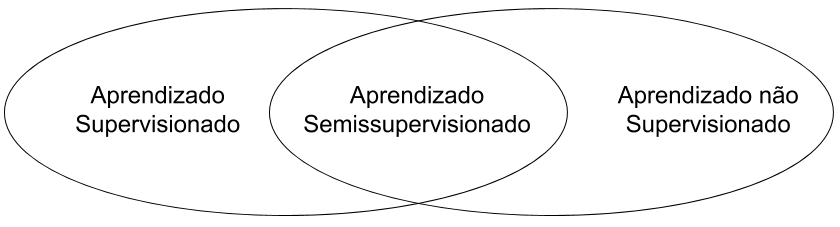
\includegraphics[scale = 0.4]{figuras/Aprendizado-de-maquina.png}
        \source{O Próprio Autor (\imprimirdata)}
        \label{fig:machine-learning}
    \end{figure}
    
    A abordagem Supervisionada exige uma base de dados com todos os exemplos rotulados para gerar um classificador com uma eficácia maior. Porém, a abordagem semissupervisionada vem demonstrando ser relevante para muitas aplicações no mundo real, pois nem sempre é possível obter a base com todos os dados rotulados, ou é necessário utilizar recursos financeiros e conhecimento dos profissionais com a finalidade de treinar um classificador com uma eficácia maior. Então, com o \ac{ssl} reduz\hyp{se} o custo e esforço necessário para executar a rotulagem em um conjunto de dados \cite{bouchachia2012semi, hady2013semi}.
    
    Além disto, essa abordagem pode ser utilizada tanto para as tarefas de classificação como as tarefas de \textit{clustering}. Para a tarefa de classificação, os classificadores são utilizados para realizar predições sobre os dados adicionando no conjunto dos dados rotulados $L$. Quando a tarefa é de \textit{clustering} os exemplos rotulados auxiliarão a definir os núcleos destes agrupamentos, obtendo assim uma eficácia melhor no agrupamento~\cite{chapelle2006semi}.
    
    Dentre os diversos algoritmos do aprendizado semissupervisionado destacam\hyp{se} \textit{Co\hyp{Training}} e \textit{Self\hyp{Training}}~\cite{zhu2008survey}. O \textit{Co\hyp{Training}} tem a sua execução dividindo verticalmente a base de dados $D$ em $D_1$ e $D_2$, de modo que os atributos em $D_1$ são diferentes dos de $D_2$~\cite{blum1998cotraining}.
    
    % com os aprendizes baseados em árvore de decisão, regras de associação, no método bayesiano e instâncias
    
    Neste trabalho será dado um foco maior ao algoritmo \textit{Self\hyp{Training}}, também conhecido por \textit{Self\hyp{Learning}}, \textit{Self\hyp{Labeling}} ou \textit{Decision\hyp{Directed}}. Um algoritmo do \ac{ssl} onde sua execução é dada por: i) iniciar com um conjunto pequeno de dados rotulados; ii) treina o classificador com os exemplos do conjunto dos rotulados $L$; iii) conforme suas previsões realiza a classificação dos exemplos que não possuem classe; iv) adiciona os exemplos no conjunto dos rotulados $L$~\cite{chapelle2006semi, grandvalet2005semi, zhu2009introduction}. No Pseudocódigo~\ref{alg:self-training} encontra-se o algoritmo do \textit{Self\hyp{Training}}.
	
	%% pseudo-código by araujobd
    %
    \begin{algorithm}[H]
        \caption{Pseudocódigo do \textit{Self\hyp{Training}}}
        \label{alg:self-training}
        \SetAlgoLined
        \begin{algorithmic}[1]
            \REQUIRE \textit{dados rotulados} $\{(\mathbf{x}_i, y_i)\}^l_{i = 1}$, \textit{dados não rotulados} $\{\mathbf{x}_j\}^{l+u}_{j=l+1}$
            \ENSURE $L \leftarrow \{(\mathbf{x}_i, y_i)\}^l_{i = 1}$ \textit{e} $U \leftarrow \{\mathbf{x}_j\}^{l+u}_{j = l+1}$
            \REPEAT
            	\STATE \textit{Treinar $f$ de $L$ usando aprendizado supervisionado}
            	\STATE \textit{Aplique $f$ as instâncias não rotuladas em $U$}
            	\STATE \textit{Remova um subconjunto $S$ de $U$; adicione $\{(\mathbf{x}, f(\mathbf{x}))|\mathbf{x}\in S\}$a $L$}
            \UNTIL{$U = \emptyset$}
        \end{algorithmic}
    \end{algorithm}
	\begin{center}
        \vspace{-2em}
        \source{Adaptado de~\cite{zhu2009introduction}}
	\end{center}
	
    \vspace{-2em}
    \noindent
	onde, $L$ representa o conjunto de dados inicialmente rotulados, $U$ representa o restante da base de dados contendo os exemplos não rotulados, $f$ é o classificador que vai realizar o aprendizado de modo supervisionado a partir do conjunto $L$, $S$ representa o subconjunto de $U$ que será incluído em $L$, $\{(\mathbf{x}_i, y_i)\}^l_{i = 1}$ o \textit{i}\hyp{ésimo} par elemento e sua respectiva classe no conjunto dos rotulados e $\{\mathbf{x}_j\}^{l+u}_{j=l+1}$ representa o \textit{j}\hyp{ésimo} elemento que pertence ao conjunto dos não rotulados.
% 	\begin{algorithm}
%         \caption{Pseudo\hyp{Código} do \textit{Self\hyp{Training}}}
%         \label{alg:self-training}
%         \begin{algorithmic}[1]
%             \REQUIRE \textit{dados rotulados} $\{(\mathbf{x}_i, y_i)\}^l_{i = 1}$, \textit{dados não rotulados} $\{\mathbf{x}_j\}^{l+u}_{j=l+1}$
%             \ENSURE \textit{Primeiramente,} $L \leftarrow \{(\mathbf{x}_i, y_i)\}^l_{i = 1}$ \textit{e} $U \leftarrow \{\mathbf{x}_j\}^{l+u}_{j = l+1}$
%             \REPEAT
%             	\STATE \textit{Treinar $f$ de $L$ usando aprendizado supervisionado}
%             	\STATE \textit{Aplique $f$ às instâncias não rotuladas em $U$}
%             	\STATE \textit{Remova um subconjunto $S$ de $U$; adicione $\{(\mathbf{x}, f(\mathbf{x}))|\mathbf{x}\in S\}$a $L$}
%             \UNTIL{$U \neq \emptyset$}
%         \end{algorithmic}
%     \end{algorithm}
%     \vspace{-2em}
%     \begin{center}
%         \small{\textbf{Fonte:} Adaptado de~\cite{zhu2009introduction}}
%     \end{center}
    
    \section{Modelos de Aprendizagem}
    \label{sec:classifiers}
    
    Os Modelos de Aprendizagem possuem categorias de classificadores que são responsáveis por aprender os padrões existentes no conjunto de treinamento. Isto é, o classificador é gerado a partir da aplicação do conjunto de treinamento em um algoritmo de \ac{am}. Há, na literatura, diversas formas de agrupar os classificadores, a Figura~\ref{fig:types-of-learners} apresenta algumas das sub-divisões existentes considerando as diversas sub-áreas de aprendizado, bem como, as categorias do \ac{am}. A parte destacada será utilizada neste trabalho.
    
    \begin{figure}[!h]
        \centering
        \caption{Categorias dos Modelos de Aprendizagem.}
        \includegraphics[scale = 0.33]{figuras/Types-of-learners.png}
        \source{Adaptado de~\cite{gollapudi2016practical}}
        \label{fig:types-of-learners}
    \end{figure}

    % Os \textbf{Método de Agrupamento} de modo análogo como o paradigma de Agrupamento o objeto deste método é de dividir em grupos os objetos semelhantes, além disto, um objeto não possui ligação ou referência em outro agrupamento, desta forma garante-se que cada conjunto possua diversos elementos e cada elemento pertence unicamente a um único agrupamento~\cite{celinski1998clustering}.

    % Os \textbf{Métodos de Conjuntos} se mostram muito eficientes na precisão da tarefa de classificação. Como o próprio nome sugere, esse método cria conjuntos de classificadores, após aplicar tal conjunto nos novos dados~\cite{gislason2006ensable, dietterich2000ensemble}.

    % A categoria de algoritmos dos \textbf{Métodos de Kernels} podem ser aplicadas em diversas atividades como classificação. agrupamentos, regressão, dentre outras. Há diferentes kernels na literatura, cada um deles ajusta-se melhor para determinada base de dados, além disto, esses métodos foram desenvolvidos para fazer o processamento de matrizes quadradas simétricas positivas~\cite{vert2004kernel}.

    %Uma rede neural tem entrada, processamento e saída. A entrada são os atributos na base de dados, o processamento é a aplicação dos pesos para cada entrada e a saída é casualmente binária, podendo ser uma nova entrada para outro neurônio, para o caso de redes com mais de uma camada.

    % \textbf{Redes Neurais Artificiais} resolvem problemas de classificação e de regressão. Essa categoria possui algumas características as quais se assemelham com o cérebro humano, dentre elas, o processo que simula uma sinapse que seria a propagação do pulso elétrico ou não, a simulação de um ou mais neurônios~\cite{russell2009artificial}.

    % O aprendizado baseado em \textbf{Redução de Dimensionalidade}, como o próprio nome sugere, são necessários para extrair quais os atributos que representam bem as instâncias garantindo integridade na hora da classificação. Bases de dados possuem uma dimensionalidade alta quando a quantidade de atributos é elevada e nem todos os atributos são relevantes para conseguir classificar a instância. Além disto, é importante destacam que há dois tipos de redução, uma que foca em reduzir atributos e a outra onde o principal objetivo é reduzir a quantidade de instâncias na base~\cite{garcia2015data, kantardzic2011data}.

    % Ao aplicar algoritmos de redução de dimensionalidade ao fim de sua execução irá obter-se uma base de dados $D'$ onde nela irá constar apenas os atributos que possuem um grau de influência elevado para a classificação do exemplo. Portanto, por existir uma quantidade menor de atributos ou instâncias na base os algoritmos de classificação/regressão vão sofrer uma diminuição no seu tempo de execução, tornando o processamento mais eficiente.

    % A \textbf{Análise de Regressão} pode ser explicada com a definição de regressão apresentada na Seção~\ref{sec:machine-learning}. A regressão é a utilização de funções algébricas no intuito de encontrar uma relação entre cada exemplo $x$ e sua classe $y$, pertencentes ao conjunto de treinamento $D$~\cite{mohri2012foundations, murphy2012probabilistic}.
    
    \subsection{Baseado em Árvores de Decisão}
        \label{subsec:decisive-tree}
        Árvores de Decisão são baseadas no método da inferência indutiva, onde cada nó da árvore representa um atributo a ser examinado, suas ramificações correspondem aos possíveis valores nos quais o atributo assume e a classe localiza\hyp{se} na folha. A medida que uma instância vai percorrendo a árvore ela é classificada~\cite{mitchell1997machine, quinlan1986induction}. Árvores de decisão possuem o desempenho mais efetivo sobre bases de dados cujo conjunto de atributos pode ser numérico e/ou categórico.

        %explicar funcionamento do rpartxse
        Dessa categoria, será utilizado o algoritmo \textit{rpartXse}, o qual~\citeonline{torgo2013package} o descreve como uma modificação do algoritmo \ac{rpart}, que realiza uma única chamada do classificador juntamente da regra da poda da árvore. Por sua vez o \ac{rpart} é uma implementação de uma árvore baseando\hyp{se} no livro Classification and Regression Trees, onde a regra da poda da árvore (1-SE) é descrita~\cite{breiman1984tree, therneau2000tree}.

        %Dependendo do algoritmo que seja escolhido, após sua execução verificando a distribuição da árvore por meio de uma busca em largura obtém\hyp{}se a ordem dos atributos de maior influência na classificação partindo do nó central até as folhas.

    \subsection{Baseado no Método Bayesiano}
        \label{subsec:bayesiano-method}
        A partir do teorema de Bayes oriundo da estatística a chance de um evento $A$ acontecer, dado $B$ ter ocorrido, supondo que $A$ e $B$ são eventos distintos, é apresentado na Equação~\ref{eq:bayes}. Um classificador Bayesiano calcula a probabilidade do exemplo pertencer a cada uma das classes existentes na base, e associa-o à classe que obtiver o melhor resultado~\cite{alpaydin2004introduction, au2017bayes, zellner1996bayes}.
        \begin{equation}
            \label{eq:bayes}
            P(A|B) = \frac{P(B|A) * P(A)}{P(B)}
        \end{equation}
        
        %explicar funcionamento do naivebayes
        O Na\"ive Bayes é um dos classificadores desta categoria. O seu modo de associar uma classe a um exemplo é calculando a probabilidade a partir da contagem da frequência e das combinações dos valores nos atributos. O classificador Na\"ive Bayes assume que todos os atributos são independentes entre si e a classe como dependente, entretanto, são raros os casos nos quais os atributos da base são independentes entre si. Ainda assim ele é bastante utilizado, uma vez que sua execução é eficiente e rápida para muitos dos problemas supervisionados~\cite{dimitoglou2012naive}.


    \subsection{Baseado em Instâncias}
        \label{subsec:instace-methods}
        Tal categoria também é conhecida como Aprendizado Preguiçoso, ou Aprendizado Baseado em Memória. Eles possuem tal característica por utilizarem todos os dados para gerar cada previsão, encontrando um conjunto de vizinhos próximos, baseando-se em funções matemáticas de distâncias entre pontos onde os vizinhos mais próximos tem uma relevância maior~\cite{atkeson1997lazy, russell2009artificial}. Os classificadores baseados em instâncias possuem o melhor desempenho sobre bases de dados com atributos numéricos e, preferencialmente normalizados, uma vez que utilizam medidas de distância com o objetivo de identificar as instâncias próximas entre si.

        %explicar funcionamento do knn
        O \ac{knn} é um dos algoritmos do aprendizado em instâncias, cuja ideia é utilizar uma quantidade de instâncias \textit{k} que sejam as mais próximas, mediante a distância, do exemplo que está sendo avaliado. Existem diversas métricas utilizadas na realização desse cálculo, dentre elas: a distância Euclidiana, a distância de \textit{Chebychev} também conhecida como valor máximo, a distância de \textit{Manhattan} que é calculada através da diferença do par dos pontos dados~\cite{aha1991, mulak2015analysis}.

    \subsection{Regras de Associação}
        \label{subsec:association-rules}
        O aprendizado baseado nesta sub\hyp{divisão} funciona de forma que os algoritmos realizam uma avaliação dos atributos da base de dados, gerando assim um conjunto de regras. Em seguida, este conjunto de regras será submetido a testes para verificar o quão válidas tais regras são para a base, a fim de validar este conhecimento~\cite{gollapudi2016practical}. Esse processo se repete até que todas as classes da base de dados possua um conjunto de regras.
        
        %explicar funcionamento do ripper
        Nessa categoria, existe o algoritmo \acs{ripper} (do inglês, \textit{\acl{ripper}}), que é uma evolução desenvolvida do \acs{irep} (do inglês \textit{\acl{irep}}), por sua vez, baseá\hyp{se} na técnica \acs{rep} (do inglês, \acl{rep}) já existente nos algoritmos baseados em árvores~\cite{cohen1995ripper}. A sua execução é dada por uma análise inicial nas classes, gerando um conjunto de regras, a partir do qual esse algoritmo analisa se todos os exemplos são cobertos pelo conjunto de regras da classe específica. Finalizada essa etapa, o algoritmo troca a classe e reinicia o processo, até que todas as classes obtenham os seus conjuntos de regras~\cite{rajput2011j48}.
    
    % ÚLTIMO TÓPICO
    \section{Trabalhos Relacionados}
    \label{sec:related-works}
    
    \citeonline{rodrigues2013selftraining, rodrigues2014selftraining, tao2018selftraining} e \citeonline{vale2018selftraining} propõem pesquisas que fazem uso do algoritmo \textit{Self\hyp{Training}} para problemas de classificação de rótulo único ou multi\hyp{rótulo}.
    
    Em~\citeonline{rodrigues2013selftraining} foi utilizado o algoritmo \textit{Self\hyp{Training}} com métodos propostos pelos próprios autores para a classificação multirrótulo. O trabalho propoz reduzir a aleatoriedade da escolha dos exemplos durante o processo de rotulagem, fazendo uso de um limiar, aliado ao fator de confiança (o pertencimento de um exemplo a sua classe) para decidir se a instância deveria ir para o conjunto dos rotulados, ou não. Por fim, foi realizada uma análise comparativa entre os três métodos, utilizando\hyp{se} cinco bases com seis métricas de avaliação. 
    
    \citeonline{rodrigues2014selftraining} identificaram que o uso do limiar de inclusão causou uma limitação no número de instâncias adicionadas, uma vez que uma quantidade bem menor de instâncias é adicionada, necessitando assim de uma quantidade maior de iterações. Como solução, foi proposto retirar esse limiar e fazer uso apenas do fator de confiança, ordenando os exemplos de forma decrescente com base nesse valor e selecionando \textit{x} exemplos por iteração.
    
    Em~\citeonline{tanha2017semi}, os autores apresentaram que uma árvore de decisão (classificador supervisionado) não produz boas estimativas de probabilidade para as previsões quando aplicadas ao \textit{Self\hyp{Training}}. Foram desenvolvidas várias modificações nesse classificador com a finalidade de produzir uma estimativa melhor. As técnicas utilizadas foram: i) não poda da árvore; ii) correção de \textit{Laplace}; iii) uma medida baseada em distância. 
    
    Em~\citeonline{tao2018selftraining}, foi proposto uma modificação do \textit{Self\hyp{Training}}, os autores utilizam dados rotulados e não rotulados para realizar a classificação dos dados, além de utilizar duas medidas para auxiliar o algoritmo, sendo elas: i) um método baseado na caminhada aleatória, utilizado junto ao classificador para gerar previsões confiáveis nos dados não rotulados ii) o sub\hyp{conjunto} ótimo $U'$ que gera mais instâncias no conjunto de treinamento.
    
    No trabalho de~\citeonline{vale2018selftraining}, foi realizada uma comparação entre o algoritmo \textit{Self\hyp{Training}} e três variações desse algoritmo propostos pelos autores. Essas variações diferenciam\hyp{se} por realizarem uma nova forma de calcular o limiar controlado dinamicamente, incluindo assim novos exemplos no conjunto dos rotulados. Os resultados das variações propostas obtiveram taxas de acerto melhores que o algoritmo do \textit{Self\hyp{Training}} utilizado nos testes. 
    
    % O foco desta pesquisa é realizar uma análise comparativa de dois algoritmos propostos em \citeonline{vale2018selftraining}. Diferindo\hyp{se} por utilizar diferentes valores para a variação do limiar e aplicando a quatro classificadores sendo eles: rpartXse, Naive Bayes, \ac{knn} e \ac{ripper}.
    
    
    O foco desta pesquisa é realizar uma análise comparativa de dois algoritmos propostos em \citeonline{vale2018selftraining} que utiliza um classificador para avaliar se o limiar é alterado ou não. Diferindo\hyp{se} por realizar uma análise dos efeitos de diferentes valores aplicados a taxa de variação do limiar, para avaliar as acurácias obtidas pelos classificadores: Na\"ive Bayes, \textit{rpartXse}, \ac{knn} e \ac{ripper}.


    % Elemento Obrigatório para TCC I e II
    %%%%%%%%%%%%%%%%%%%%%%%%%%%%%%%%%%%%%%%%%%%
%%                                       %%
%%      Desenvolvimento da Pesquisa      %%
%%                                       %%
%%%%%%%%%%%%%%%%%%%%%%%%%%%%%%%%%%%%%%%%%%%

%% Neste capítulo expõe-se os experimentos da sua pesquisa a proposta de solução da sua pesquisa e em caso do TCC II como ela foi implementada
\chapter{Desenvolvimento da Pesquisa}
    \label{cha:desenvolvimento-da-pesquisa}
    
    Neste capítulo será descrito em detalhes o que foi desenvolvido e como a idea foi executada. Ao fim do capítulo, são apresentados alguns resultados parciais após a aplicação da proposta.

    % Neste Tópico é onde o aluno irá discorrer exatamente o problema no qual a sua pesquisa pretende resolver, com base nos objetivos apontados no Capítulo 1.

\section{Questões de Pesquisa}
    \label{sec:questoes-de-pesquisa}

    % Comparativo de métodos
    % variação da taxa do limiar
    % 3%, 5% e 7%
    % Métricas de avaliação (comparação com 5%)
    % Analisar os algoritmos e explicar?
    %  que foram propostos em~\citeonline{vale2018selftraining} são: FlexConf-C1 e FlexConf-C2. 

    Como explanado na Subseção~\ref{subsec:objetivo-geral}, esse trabalho realizou a comparação dos algoritmos \textit{FlexCon\hyp{C1}} e \textit{FlexCon\hyp{C2}}, realizando manipulações exclusivamente na taxa de variação do limiar, mantendo a proposta original discutida em~\cite{vale2018selftraining}, taxa de variação fixa em 5\% . Neste trabalho, foi analisada a influência na classificação de dados quando aplicadas diversos valores para a taxa de variação do limiar. A variação aplicada ao limiar foi entre 2\% e 8\%, comparando os resultados obtidos para cada um destes valores com o valor base 5\%.

    A validação da proposta deste trabalho foi por meio de uma comparação das médias das acurácias e as variâncias obtidas pelo respectivo classificador. Para realizar uma análise do ponto de vista estatístico foi realizada a análise de variância (do inglês, \ac{anova}) que é um teste de hipótese que valida se duas ou mais populações são iguais. Esse teste, tem como resultado um parâmetro \textit{p\hyp{value}} que sua faixa varia entre (0, 1], quando esse fator possui um valor menor que 0.05 é dito que a hipótese testada é estatisticamente significante, caso contrário ela não é significante.

    % Para avaliação do ponto de vista estatístico, o teste de \textit{Friedman and Nemenyi Post-Hoc} foi selecionado para essa comparação, por realizar análise de variância não paramétrica bidirecional~\cite{norheim1986friedman}.

    % Como métricas de avaliação será desenvolvida uma comparação dos algoritmos a partir média das acurácias obtidas nas bases de dados com um dos classificadores alterando apenas a variação que é incorporada ao limiar. Essa análise será realizada com o teste estatístico de \textit{Friedman and Quade}, por ser uma análise de variância não paramétrica bidirecional.
    
    
%%%%%%%%%%%%%%%%%%%%%%%%%%%%%%%%%%%
%%      Proposta de solução      %%
%%%%%%%%%%%%%%%%%%%%%%%%%%%%%%%%%%%

% Neste tópico deverão ser apresentadas suas propostas para solucionar o problema de seu trabalho, para o TCC II deverão ser apresentadas, também, as formas de implantação destas soluções.

\section{Proposta de Solução}
    \label{sec:proposta-de-solucao}

    Nesta seção descreve as bases de dados utilizadas nesta pesquisa e a ideia do método estudado. O Pseudocódigo~\ref{alg:flexcon-c} apresenta a ideia geral do \ac{flexcon}, que a sua execução é dada por: i) separar os exemplos rotulados dos exemplos não rotulados; ii) treinar o classificador $f$ utilizando o conjunto dos rotulados $L$; iii) aplicar $f$ no conjunto dos não rotulados $U$, gerando assim uma matriz com o exemplo, sua respectiva classe e confiança do classificador; iv) selecionar todos os exemplos dado a regra de inserção; v) adicionar todos os exemplos de $S$ em $L$; vi) utilizar o conjunto $S$ para treinar um classificador $f'$; vii) aplicar o classificador $f'$ em $L$; viii) atualizar o valor do limiar de inserção com base na acurácia obtida em $f'$.

    O \ac{flexcon} decide se o exemplo deve ir para o conjunto dos rotulados realizando uma varredura nas regras de inserção de exemplos que são: i) os exemplos são da mesma classe e as confianças são maiores que o limiar; ii) os exemplos possuem a mesma classe, porém apenas uma de suas confianças é maior que o limiar; iii) os exemplos possuem classes diferentes e ambas as confianças são maiores que o limiar; e iv) os exemplos possuem classes diferentes e uma das confianças é maior que o limiar. A regra de inserção subsequente só é executada se, e somente se, executar a varredura e nenhum exemplo se aplicar na regra atual e caso não consiga selecionar nenhum exemplo e todas as regras foram percorridas a confiança é alterada para o maior valor de confiança da predição da iteração corrente.

    \begin{algorithm}[H]
        \caption{\acs{flexcon}}
        \label{alg:flexcon-c}
        \SetAlgoLined
        \begin{algorithmic}[1]
            \REQUIRE \textit{dados rotulados} $\{(\mathbf{x}_i, y_i)\}^l_{i = 1}$, \textit{dados não rotulados} $\{\mathbf{x}_j\}^{l+u}_{j=l+1}$
            \ENSURE $L \leftarrow \{(\mathbf{x}_i, y_i)\}^l_{i = 1}$ \textit{e} $U \leftarrow \{\mathbf{x}_j\}^{l+u}_{j = l+1}$
            \REPEAT
            	\STATE \textit{Treinar $f$ com os exemplos de $L$ usando aprendizado supervisionado}
            	\STATE \textit{Aplicar $f$ as instâncias não rotuladas em $U$}
            	\STATE \textit{Remover um subconjunto $S$ de $U$ tal que o exemplo se enquadre com uma das regras inclusão de novos exemplos}
            	\STATE \textit{Adicionar $\{(\mathbf{x}, f(\mathbf{x}))|\mathbf{x} \in  S\}$ a $L$}
            	\STATE \textit{Treinar $f'$ com os exemplos de $S$ utilizando aprendizado supervisionado}
            	\STATE \textit{Aplicar $f'$ as instâncias em $L$}
            	\STATE \textit{Atualizar o limiar de inclusão a partir da acurácia em $f'$}
            \UNTIL{$U = \emptyset$}
        \end{algorithmic}
    \end{algorithm}
	\begin{center}
        \vspace{-2em}
        \source{Adaptado de~\cite{vale2018selftraining}}
	\end{center}
    \vspace{-2em}
    O \ac{flexcon} possui duas técnicas diferentes \textit{FlexCon\hyp{C1}} e \textit{FlexCon\hyp{C2}} para decidir qual rótulo será atribuído a cada exemplo. A técnica \textit{FlexCon\hyp{C1}} guarda a predição da primeira iteração e para comparar com a predição da iteração corrente. Quando as predições convergem entre as classes o exemplo é adicionado. Caso o exemplo seja selecionado para ser incluído no conjunto dos exemplos rotulados a sua classe é definida através da quantidade de vezes que ele obteve um determinada classe. Isso gerou duas variações da mesma técnica \textit{FlexCon\hyp{C1}}(s) que utiliza a soma das confianças obtidas desde a primeira iteração até a atual para realizar essa decisão e \textit{FlexCon\hyp{C1}}(v) que faz uso de votação onde é contabilizado somente as ocorrências do exemplo em cada classe.

    A técnica \textit{FlexCon\hyp{C2}} compara as predições do classificador da iteração corrente com a predição de um classificador supervisionado que é treinado com as instâncias inicialmente rotuladas. Quando as predições convergem entre as classes o exemplo é adicionado, caso o exemplo selecionado para a inclusão não possua a mesma classe nas predições, o rótulo é selecionado verificando o rótulo do classificador supervisionado.

    O limiar da iteração subsequente é calculado verificando se o conjunto dos exemplos adicionados na iteração atual possui uma quantidade mínima de exemplos de todas as classes, em caso positivo o classificador treina com os exemplos adicionados da iteração e testa com os exemplos inicialmente rotulados. Em caso negativo o conjunto de treino fica se acumulando até possuir a quantidade mínima de exemplos por classe.
    % \vspace{-1em}
    % \noindent
    % onde, $L$ representa o conjunto de dados inicialmente rotulados, $U$ representa o restante da base de dados contendo os exemplos não rotulados, $f$ é o classificador que vai realizar o aprendizado de modo supervisionado a partir do conjunto $L$, $S$ representa o subconjunto de $U$ que será incluído em $L$, $\{(\mathbf{x}_i, y_i)\}^l_{i = 1}$ o \textit{i}\hyp{ésimo} par elemento e sua respectiva classe no conjunto dos rotulados e $\{\mathbf{x}_j\}^{l+u}_{j=l+1}$ representa o \textit{j}\hyp{ésimo} elemento que pertence ao conjunto dos não-rotulados.

    O limiar de inclusão da primeira iteração é de 95\%, isto é, as instâncias que na primeira iteração possuírem uma confiança igual ou maior que este valor irão para o conjunto dos dados rotulados. A partir da segunda iteração, o algoritmo irá realizar o cálculo do novo limiar de inclusão considerando a acurácia do classificador e esse limiar foi variado conforme representado na Equação~\ref{eq:conf} proposta em~\cite{vale2018selftraining}.

    \begin{equation}
        \label{eq:conf}
    	\hspace{-0.2cm} conf(t_{i+1}) \hspace{-0.1cm}= \hspace{-0.1cm}
    	\left \{
    	\begin{array}{lr}
    	\hspace{-0.2cm}conf(t_i) - cr, & \hspace{-0.8cm}\text{if } acc \geq mp + e \\
    	\hspace{-0.2cm}conf(t_i), & \hspace{-0.3cm} \text{se } mp - e < acc < mp + e \\
    	\hspace{-0.2cm}conf(t_i) + cr, & \hspace{-0.8cm}\text{if } acc \leq mp - e \\
    	\end{array}
    	\right.
    	\hspace{-0.5cm}
	\end{equation}

    \noindent
    onde, $conf(t_{i+1})$ é a confiança da próxima iteração, $conf(t_i)$ é a confiança da iteração atual, $cr$ é a taxa de variação na qual o limiar é aplicado, $acc$ é a acurácia do classificador, $mp$ precisão mínima e $e$ é uma variação de precisão aceitável que é permitida para definir uma estabilização em precisão.

    Em \citeonline{vale2018selftraining} o $cr$ foi fixo em 5\%, isto é, o limiar variava em 5 pontos percentuais por iteração. Entretanto, este trabalho pretende utilizar diversos valores [$2\%, 8\%$] do parâmetro $cr$ para analisar o seu efeito na classificação dos dados.

    % FlexConf-C1
    % usa 2 predições a da iteração atual e a 1 iteração
    % duas versões soma e voto
    % nova taxa de confiança é calculada utilizando os novos rotulados para treinamento e o dl para teste

    % \section{Experimentos Parciais}
    % \label{sec:experimentos}
    % Montar uma tabela com as i) bases utilizadas, ii) quantidade de instâncias, iii) quantidade de atributos, iv) quantidade de classes, v) tipo da base (Categórico, Numérico, Discreto, etc)

    % Ressaltar o uso das taxas de instâncias inicialmente rotuladas de 5% até 25% de 5% em 5% além de variar a taxa que é incorporada ao limiar (taxa de variação da confiança) que é de 3%, 5% e 7% (e talvez de uma taxa variável).
    Com a finalidade de avaliar a eficácia das variações propostas, foi realizada uma análise empírica. A partir da aplicação do método \ac{flexcon} sobre um conjunto de 31 bases de dados. A Tabela~\ref{tab:bases-de-dados} descreve os conjuntos de dados previamente selecionados, em termos do número de exemplos (Instâncias), de atributos e a quantidade de classes para cada conjunto de dados, além de indicar os tipos de dados como categórico (C), inteiro (I) ou real (R).

    \begin{table}[h]
        \caption{Bases de Dados que serão utilizadas nos experimentos.}
        \centering
        \begin{tabular}{|c|c|c|c|c|} \hline
            \textbf{Base de dados} & \textbf{Instâncias} & \textbf{Atributos} & \textbf{Classes} & \textbf{Tipo} \\ \hline
            Balance Scale                &  625  &   4 &  3 & I \\ \hline
            Blood Transfusion Service    &  748  &   5 &  2 & R \\ \hline
            Bupa                         &  345  &   7 &  2 & C, I, R \\ \hline
            Car                          & 1728  &   6 &  4 & C, R \\ \hline
            Cnae-9                       & 1080  & 857 &  9 & I \\ \hline
            Connectionist-mines-vs-rocks &  208  &  60 &  2 & R \\ \hline
            Flare                        & 1389  &  10 &  6 & C \\ \hline
            Haberman                     &  306  &   4 &  2 & I \\ \hline
            Handwritten Digits           & 10992 &  16 & 10 & I \\ \hline
            Hill Valley                  &  606  & 101 &  2 & R \\ \hline
            Image Segmentation           & 2310  &  19 &  7 & R \\ \hline
            Indian Liver Patient         &  582  &  10 &  2 & I, R \\ \hline
            Iris                         &  150  &   5 &  3 & R \\ \hline
            King-Rook vs King Pawn       & 3196  &  36 &  2 & C \\ \hline
            Leukemia Haslinger           &  100  &  50 &  2 & R \\ \hline
            Mammographic Mass            &  961  &   6 &  2 & I \\ \hline
            Mfeat-karhunen               & 2000  &  64 & 10 & I, R \\ \hline
            Mushroom                     & 8124  &  22 &  2 & C \\ \hline
            Musk                         & 6598  & 168 &  2 & I \\ \hline
            Ozone Level Detection        & 2536  &  73 &  2 & R \\ \hline
            Phishing                     & 2456  &  30 &  3 & I \\ \hline
            Pima                         &  768  &   9 &  2 & I, R \\ \hline
            Planning-relax               &  182  &  13 &  2 & R \\ \hline
            Seeds                        &  210  &   7 &  3 & R \\ \hline
            Semeion                      & 1593  & 256 & 10 & I \\ \hline
            Spectf Heart                 &  267  &  14 &  2 & I \\ \hline
            Tic-tac-toe                  &  958  &   9 &  2 & C \\ \hline
            Twonorm                      & 7400  &  21 &  2 & R \\ \hline
            Vehicle                      &  946  &  18 &  4 & I \\ \hline
            Waveform                     & 5000  &  40 &  3 & R \\ \hline
            Wilt                         & 4839  &   6 &  2 & R \\ \hline
        \end{tabular}
        \label{tab:bases-de-dados}
        \source{O Próprio Autor (\imprimirdata)}
    \end{table}

    A solução proposta foi desenvolvida na linguagem de programação R, em virtude de ser um software livre (\textit{open source}) que vem apresentando crescimento ao longo dos anos. Além disso, a referida linguagem fornece diversas ferramentas e bibliotecas para facilitar as análises estatísticas.
    
    \section{\textit{Design} de Experimento}
    \label{sec:design-experimento}

    Nesta seção está descrito o \textit{design} (modelo lógico) utilizado para a execução dos experimentos, conforme apresentado no Algoritmo~\ref{alg:design}.
    
    Cada um dos classificadores selecionados para esse estudo (Naïve Bayes, \textit{rpartXse}, \ac{knn} e \ac{ripper}) é avaliado individualmente, utilizando\hyp{se} a técnica de validação cruzada (do inglês, \textit{cross\hyp{validation}}). Essa técnica é utilizada para a validação de dados obtidos em experimentos, dividido\hyp{se} a base de dados em $k$ \textit{folds} e mantendo\hyp{se} a estratificação (proporção de cada classe) nos mesmos. Além disto, cada \textit{fold} é utilizado como conjunto de teste para verificar a acurácia do classificador, sendo utilizados $k - 1$ \textit{folds} para treinamento e $1$ \textit{fold} para teste do classificador~\cite{wong2015cross}.
    
    O algoritmo recebe por parâmetro o classificador e a execução segue os seguintes passos: i) para cada base de dados, carregue\hyp{a} em memória; ii) separe os \textit{folds} na base selecionada; iii) para cada valor do parâmetro $cr$, itere os percentuais de exemplos inicialmente rotulados; iv) para cada um dos percentuais de exemplos inicialmente rotulados, percorra os \textit{folds} criados; v) para cada um dos \textit{folds}, separe os conjuntos de treino e teste; vi) gere os modelos a partir do método \ac{flexcon}; vii) teste a acurácia dos modelos com o conjunto selecionado para teste; viii) grave as informações em arquivo.
    
    Com este \textit{design}, garante\hyp{se} a mesma distribuição dos \textit{folds} para as técnicas implementadas, quando fixados os valores do parâmetro $cr$ e da taxa de exemplos inicialmente rotulados. Além disto, o \ac{flexcon} teve que ser adaptado para receber dois parâmetros, o valor do $cr$ e o classificador a ser utilizado.

    % Cada uma destas bases de dados será dividida em dois sub\hyp{conjuntos} i) para treinamento do classificador, com 75\% das instâncias; e ii) para teste do classificador, com 25\% das instâncias. Após essa etapa, dos 75\% dos dados de treinamento será selecionado um percentual para permanecer com o rótulo 5\%, 10\%, 15\%, 20\% ou 25\%. Uma vez separados os conjuntos dos rotulados e não rotulados, os dados poderão ser aplicados ao algoritmo para realização da tarefa de classificação. Para isso, pretende\hyp{se} utilizar os classificadores Naïve Bayes, rpartXse, \ac{ripper} e o \ac{knn}.

    % Cada uma destas bases de dados foi aplicado o \textit{cross\hyp{validation}} com $k$ \textit{folds} onde $1$ \textit{fold} é separado para teste e $k - 1$ \textit{folds} para treinamento~\cite{wong2015cross}.
    
    \begin{algorithm}[H]
        \caption{\textit{Design} de Experimento utilizado}
        \label{alg:design}
        \SetAlgoLined
        \begin{algorithmic}[1]
            \REQUIRE \textit{classificador cl}
            \FORALL{base em base\_de\_dados}
                \STATE \textit{base\_carregada $\leftarrow$ carregar\_base(base)}
                \STATE \textit{folds $\leftarrow$ separar\_folds(base\_carregada)}
                \FORALL{$cr$ em \textit{change\_rate}}
                    \FOR{\textit{i $\leftarrow$ 1 até 5}}
                        \STATE \textit{ini\_rot $\leftarrow$ i * 5}
                        \FORALL{\textit{fold} em \textit{folds}}
                            \STATE \textit{\textit{teste} $\leftarrow$ fold}
                            \STATE \textit{treinamento $\leftarrow$ folds - fold}
                            \STATE \textit{L $\leftarrow$ selecionar\_exemplos(treinamento, ini\_rot)}
                            \STATE \textit{U $\leftarrow$ treinamento - L}
                            \STATE \textit{modelo\_c1\_s $\leftarrow$ flexcon\_c1\_s(L, U, cr, cl)}
                            \STATE \textit{modelo\_c1\_v $\leftarrow$ flexcon\_c1\_v(L, U, cr, cl)}
                            \STATE \textit{modelo\_c2 $\leftarrow$ flexcon\_c2(L, U, cr, cl)}
                            \STATE \textit{acc\_c1\_s[i] $\leftarrow$ testar\_acc(modelo\_c1\_s, teste)}
                            \STATE \textit{acc\_c1\_v[i] $\leftarrow$ testar\_acc(modelo\_c1\_v, teste)}
                            \STATE \textit{acc\_c2[i] $\leftarrow$ testar\_acc(modelo\_c2, teste)}
                        \ENDFOR
                    \ENDFOR
                    \STATE \textit{gravar\_arquivo(acc\_c1\_s, acc\_c1\_v, acc\_c2)}
                \ENDFOR
            \ENDFOR
        \end{algorithmic}
    \end{algorithm}
	\begin{center}
        \vspace{-2em}
        \source{O Próprio Autor (\imprimirdata)}
	\end{center}

    \vspace{-2em}
    Após essa etapa de separação dos \textit{folds} para treinamento do classificador, foi selecionado um percentual de exemplos para permanecer rotulado. Uma vez separados os dados em dois conjuntos: rotulados e não rotulados, estes são aplicados ao algoritmo para realização da tarefa de classificação, utilizando\hyp{se} os classificadores selecionados.

    Nos experimentos foram utilizados os seguintes parâmetros: 
    
    \begin{enumerate}[label=\roman*.]
        \item \textit{k} = 10 \textit{folds} para o \textit{cross\hyp{validation}}, conforme proposto por~\cite{kohavi1995study, braga2004cross, fushiki2011cross, wong2015cross};
        \item Percentuais de 5\%, 10\%, 15\%, 20\% e 25\% instâncias inicialmente rotuladas, conforme descrito em~\cite{vale2018selftraining};
        \item Classificadores Na\"ive Bayes, \textit{rpartXse}, e \ac{ripper}, os mesmos utilizados no trabalho de~\cite{vale2018selftraining}, além da inclusão do classificador \ac{knn}.
    \end{enumerate}
    
    O valor de \textit{k} (quantidade de instâncias mais próximas) definido para o \ac{knn} é descrito pela Equação~\ref{eq:k-value}, conforme proposto em~\cite{bhattacharya2012knnvalue}:
    
    \begin{equation}
        \label{eq:k-value}
        k = \sqrt{N}
    \end{equation}

    \noindent
    onde, $N$ representa a quantidade total de instâncias na base de dados.
    %    O \textit{FlexConf\hyp{C1}} é utilizado o além do modelo gerado na iteração corrente também é levado em consideração as predições da primeira iteração. E ainda, esses classificadores individuais são combinados por soma e maioria de votos, levando a duas versões desse método, \textit{FlexConf\hyp{C1}(v)} e \textit{FlexConf\hyp{C1}(s)}. O \textit{FlexConf\hyp{C2}} utiliza o modelo da iteração corrente e um classificador supervisionado para realizar a tarefa de classificação.
    
    
%%%%%%%%%%%%%%%%%%%%%%%%%%%%%%%%%%%%%%%%%%
%%                                      %%
%%          Resultados Obtidos          %%
%%                                      %%
%%%%%%%%%%%%%%%%%%%%%%%%%%%%%%%%%%%%%%%%%%

% Neste capítulo são expostos os resultados de sua pesquisa. 
% No caso do TCC I, resultados esperados ou parciais, para TCC II, resultados "finais".

\chapter{Resultados}
    \label{cha:resultados}
    Neste capítulo serão discutidos os resultados obtidos após a aplicação da proposta discutida no Capítulo~\ref{cha:desenvolvimento-da-pesquisa}.
    A abordagem deste capítulo possui dois momentos, o primeiro momento, descrito na Seção~\ref{sec:performance-analysis}, onde são apresentados os resultados obtidos por cada classificador individualmente e também são realizadas análises no parâmetro $cr$ por classificador, por cada variação do algoritmo \ac{flexcon}. Por fim, no segundo momento, Seção~\ref{sec:statistical-analysis}, foi conduzida uma análise estatística dos resultados obtidos.
    
    % Pegar dados do Planilhas do Google Drive e transforma-los em gráficos de linhas onde o eixo X representa a porcentagem de inicialmente rotulados, o Y a porcentagem da acurácia do algoritmo e a linha representa a porcentagem de variação do limiar
    
    % Como resultados parciais deste trabalho destacam\hyp{se} a aplicação de três taxas de variações (3\%, 5\% e 7\%) que manipulam o limiar da iteração seguinte. O algoritmo \textit{FlexCon\hyp{C1} (v)} foi aplicado a um conjunto de três bases de dados (\textit{Mammographic Mass}, \textit{Mfeat\hyp{karhunen}} e \textit{Mushroom}). A Tabela~\ref{tab:partial-results} apresenta as acurácias obtidas para cada uma das bases de dados utilizando o algoritmo \textit{FlexCon\hyp{C1} (v)} aliado ao classificador Naive Bayes.
    
    % \begin{table}[h]
    %     \centering
    %     \caption{Acurácia do \textit{FlexCon\hyp{C1} (v)} utilizando o classificador Naive Bayes.}
    %     \label{tab:partial-results}
    %     \resizebox{\textwidth}{!}{%
    %         \begin{tabular}{|c|c|c|c|c|c|c|}
    %             \toprule
    %             \multirow{2}{*}{\textbf{Base de Dados}}     & \multirow{2}{*}{\textbf{Taxa de Variação}} & \multicolumn{5}{c|}{\textbf{Inicialmente Rotulados}} \\ \cmidrule(l){3-7} 
    %                                               &                                   & \textbf{5\%}     & \textbf{10\%}   & \textbf{15\%}   & \textbf{20\%}   & \textbf{25\%}   \\ \midrule
    %             \multirow{3}{*}{Mammographic Mass} & 3\%                               & 75.83\%   & 75.42\%  & 77.08\%  & 75.83\%  & 77.92\%  \\ \cmidrule(l){2-7} 
    %                                               & 5\%                               & 75.83\%   & 75.42\%  & 77.08\%  & \textbf{76.25\%}  & 77.92\%  \\ \cmidrule(l){2-7} 
    %                                               & 7\%                               & 75.83\%   & 75.42\%  & 77.08\%  & 75.83\%  & 77.92\%  \\ \midrule
    %             \multirow{3}{*}{Mfeat\hyp{karhunen}}    & 3\%                               & 84.60\%   & 88.00\%  & 90.20\%  & \textbf{90.60\%}  & 89.40\%  \\ \cmidrule(l){2-7} 
    %                                               & 5\%                               & \textbf{85.40\%}   & \textbf{88.60\%}  & \textbf{91.20\%}  & \textbf{90.60\%}  & \textbf{90.00\%}  \\ \cmidrule(l){2-7} 
    %                                               & 7\%                               & 84.60\%   & 88.00\%  & 90.20\%  & 90.40\%  & 89.40\%  \\ \midrule
    %              \multirow{3}{*}{Mushroom}          & 3\%                               & 89.66\%   & 90.89\%  & 91.68\%  & 90.65\%  & \textbf{93.11\%}  \\ \cmidrule(l){2-7} 
    %                                               & 5\%                               & \textbf{90.74\%}   & \textbf{92.12\%}  & \textbf{92.27\%}  & \textbf{91.97\%}  & 92.61\%  \\ \cmidrule(l){2-7} 
    %                                               & 7\%                               & 89.66\%   & 90.50\%  & 91.19\%  & 91.04\%  & 91.29\%  \\ \bottomrule
    %         \end{tabular}
    %     }
    %     \source{O Próprio Autor (\imprimirdata)}
    % \end{table}
    
    % As Figuras~\ref{fig:base-mammographic}, \ref{fig:base-mfeat-karhunen} e \ref{fig:base-mushroom} apresentam gráficos sintetizando as informações contidas na Tabela~\ref{tab:partial-results} para as bases de dados \textit{Mammographic Mass}, \textit{Mfeat\hyp{karhunen}} e \textit{Mushroom} respectivamente. Nestes gráficos estão representados os percentuais de exemplos inicialmente rotulados pelas acurácias obtidas alterando a taxa de variação do limiar.
    
    % \begin{figure}[h]
    %     \centering
    %     \caption{Percentuais de Exemplos Inicialmente Rotulados x Acurácia Obtida na Base \textit{Mammographic Mass}.}
    %     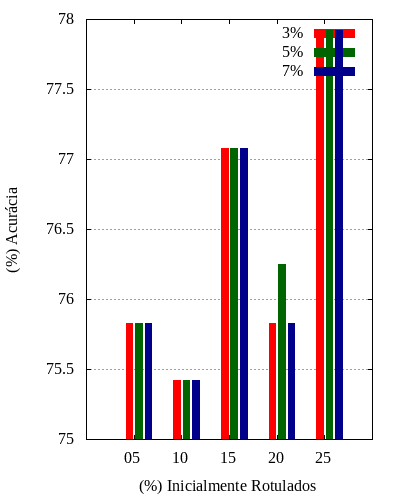
\includegraphics[scale=0.5]{figuras/Mammographic.png}
    %     \label{fig:base-mammographic}
    %     \source{O Próprio Autor (\imprimirdata)}
    % \end{figure}
    
    % \begin{figure}[h]
    %     \centering
    %     \caption{Percentuais de Exemplos Inicialmente Rotulados x Acurácia Obtida na Base \textit{Mfeat\hyp{karhunen}}.}
    %     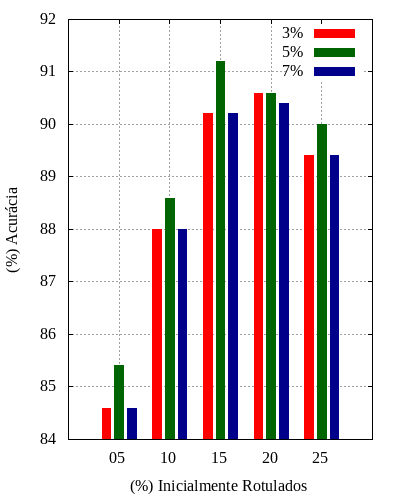
\includegraphics[scale=0.5]{figuras/Mfeat-karhunen.png}
    %     \label{fig:base-mfeat-karhunen}
    %     \source{O Próprio Autor (\imprimirdata)}
    % \end{figure}
    
    % \begin{figure}[h]
    %     \centering
    %     \caption{Percentuais de Exemplos Inicialmente Rotulados x Acurácia Obtida na Base \textit{Mushroom}.}
    %     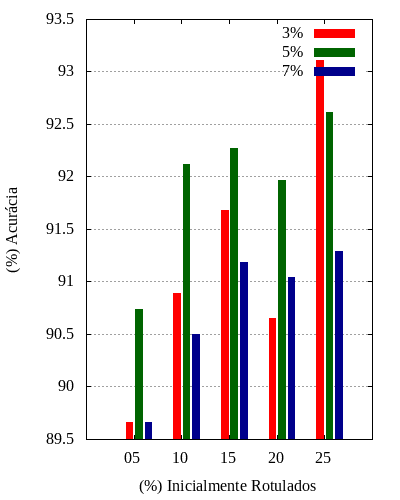
\includegraphics[scale=0.5]{figuras/Mushroom.png}
    %     \label{fig:base-mushroom}
    %     \source{O Próprio Autor (\imprimirdata)}
    % \end{figure}
    
    % As Tabelas~\ref{tab:naive-acc}-\ref{tab:knn-acc} apresentam em cada uma das células as acurácias médias obtidas pelos classificadores, além de apresentar também o desvio padrão obtido por cada classificador (Na\"ive Bayes, \textit{rpartXse}, \ac{ripper} e \ac{knn}), respectivamente. Em cada uma das referidas tabelas, está sendo analisado a variação do parâmetro $cr$ em diferentes algoritmos e diferentes percentuais de exemplos rotulados.
    \section{Analise de Performance}
        \label{sec:performance-analysis}
        
        As Tabelas~\ref{tab:naive-acc}-\ref{tab:knn-acc} apresentam o desempenho obtido pelo algoritmo \ac{flexcon} em cada uma das suas variações. Nestas tabelas, as colunas são as variações aplicadas ao parâmetro $cr$ das células as acurácias médias obtidas pelos classificadores, além de apresentar também o desvio padrão obtido por cada classificador (Na\"ive Bayes, \textit{rpartXse}, \ac{ripper} e \ac{knn}), respectivamente. Em cada uma das referidas tabelas, está sendo analisado a variação do parâmetro $cr$ em diferentes algoritmos e diferentes percentuais de exemplos rotulados.
        
        A Tabela~\ref{tab:naive-acc} apresenta os resultados obtidos após a aplicação do classificador Na\"ive Bayes. Os melhores resultados encontram\hyp{se} entre 2\% a 4\%. Realizando uma análise por algoritmo, observa\hyp{se} que quando pré\hyp{fixa} o valor do parâmetro $cr$ em 3\% obtém\hyp{se} resultados superiores em 3 dos 5 casos, para os três algoritmos. De maneira geral quando o valor do parâmetro $cr$ é pré\hyp{fixado} em 3\% os resultados são superiores em 9 dos 15 casos, representando 60\% de superioridade.
    
    \begin{table}[h]
        \centering
        \caption{Resultado da acurácia com o classificador Na\"ive Bayes}
        \resizebox{\textwidth}{!} & \textbf{3\%} & \textbf{4\%} & \textbf{5\%} & \textbf{6\%} & \textbf{7\%} & \textbf{8\%} \\ \hline
                \parbox[t]{3mm}{\multirow{5}{*}{\rotatebox[origin=c]{90}{FlexCon-C1(s)}}} & 05\% & $73,75 \pm 17,97$ & $73,37 \pm 16,75$ & $\textbf{74,66} \pm 18,02$ & $74,22 \pm 17,53$ & $73,33 \pm 17,91$ & $73,87 \pm 17,39$ & $73,34 \pm 18,29$ \\ \cline{2-9}
                 & 10\% & $\textbf{73,80} \pm 17,08$ & $73,57 \pm 17,16$ & $73,25 \pm 18,16$ & $73,58 \pm 17,64$ & $72,53 \pm 18,53$ & $73,36 \pm 17,44$ & $73,12 \pm 17,75$ \\ \cline{2-9}
                 & 15\% & $72,86 \pm 17,52$ & $\textbf{73,54} \pm 17,30$ & $72,97 \pm 17,93$ & $73,24 \pm 17,75$ & $72,46 \pm 17,68$ & $73,50 \pm 16,58$ & $73,46 \pm 16,91$ \\ \cline{2-9}
                 & 20\% & $72,90 \pm 17,43$ & $\textbf{73,90} \pm 16,82$ & $72,57 \pm 17,07$ & $72,73 \pm 17,25$ & $72,29 \pm 18,54$ & $72,71 \pm 18,17$ & $72,59 \pm 18,69$ \\ \cline{2-9}
                 & 25\% & $73,34 \pm 17,30$ & $\textbf{74,73} \pm 16,87$ & $73,71 \pm 16,69$ & $74,38 \pm 16,75$ & $73,98 \pm 16,69$ & $74,44 \pm 17,19$ & $73,77 \pm 17,85$ \\ \hline
                \parbox[t]{3mm}{\multirow{5}{*}{\rotatebox[origin=c]{90}{FlexCon-C1(v)}}} & 05\% & $73,75 \pm 17,97$ & $73,37 \pm 16,75$ & $\textbf{74,66} \pm 18,02$ & $74,22 \pm 17,53$ & $73,33 \pm 17,91$ & $73,87 \pm 17,39$ & $73,34 \pm 18,29$ \\ \cline{2-9}
                 & 10\% & $\textbf{73,80} \pm 17,08$ & $73,57 \pm 17,16$ & $73,25 \pm 18,16$ & $73,58 \pm 17,64$ & $72,53 \pm 18,53$ & $73,36 \pm 17,44$ & $73,12 \pm 17,75$ \\ \cline{2-9}
                 & 15\% & $72,86 \pm 17,52$ & $\textbf{73,54} \pm 17,30$ & $72,97 \pm 17,93$ & $73,24 \pm 17,75$ & $72,46 \pm 17,68$ & $73,50 \pm 16,58$ & $73,46 \pm 16,91$ \\ \cline{2-9}
                 & 20\% & $72,90 \pm 17,43$ & $\textbf{73,90} \pm 16,82$ & $72,57 \pm 17,07$ & $72,73 \pm 17,25$ & $72,29 \pm 18,54$ & $72,71 \pm 18,17$ & $72,59 \pm 18,69$ \\ \cline{2-9}
                 & 25\% & $73,34 \pm 17,30$ & $\textbf{74,73} \pm 16,87$ & $73,71 \pm 16,69$ & $74,38 \pm 16,75$ & $73,98 \pm 16,69$ & $74,44 \pm 17,19$ & $73,77 \pm 17,85$ \\ \hline
                \parbox[t]{3mm}{\multirow{5}{*}{\rotatebox[origin=c]{90}{FlexCon-C2}}} & 05\% & $73,75 \pm 17,97$ & $73,37 \pm 16,75$ & $\textbf{74,66} \pm 18,02$ & $74,22 \pm 17,53$ & $73,33 \pm 17,91$ & $73,87 \pm 17,39$ & $73,34 \pm 18,29$ \\ \cline{2-9}
                & 10\% & $\textbf{73,80} \pm 17,08$ & $73,57 \pm 17,16$ & $73,25 \pm 18,16$ & $73,58 \pm 17,64$ & $72,53 \pm 18,53$ & $73,36 \pm 17,44$ & $73,12 \pm 17,75$ \\ \cline{2-9}
                & 15\% & $72,86 \pm 17,52$ & $\textbf{73,54} \pm 17,30$ & $72,97 \pm 17,93$ & $73,24 \pm 17,75$ & $72,46 \pm 17,68$ & $73,50 \pm 16,58$ & $73,46 \pm 16,91$ \\ \cline{2-9}
                & 20\% & $72,90 \pm 17,43$ & $\textbf{73,90} \pm 16,82$ & $72,57 \pm 17,07$ & $72,73 \pm 17,25$ & $72,29 \pm 18,54$ & $72,71 \pm 18,17$ & $72,59 \pm 18,69$ \\ \cline{2-9}
                & 25\% & $73,34 \pm 17,30$ & $\textbf{74,73} \pm 16,87$ & $73,71 \pm 16,69$ & $74,38 \pm 16,75$ & $73,98 \pm 16,69$ & $74,44 \pm 17,19$ & $73,77 \pm 17,85$ \\ \hline
            \end{tabular}%
        }
        \label{tab:naive-acc}
        \source{O Próprio Autor (\the\year)}
    \end{table}
    
    A Tabela~\ref{tab:rpart-acc} apresenta os resultados obtidos pelo classificador \textit{rpartXse}. Para o algoritmo \textit{FlexCon\hyp{C1} (s)} os melhores valores para o parâmetro $cr$ concentram\hyp{se} em 4\% e 8\% quando pré\hyp{fixa} o parâmetro $cr$ nestes valores os resultados são superiores em 2 dos 5 casos, para ambos valores. O algoritmo \textit{FlexCon\hyp{C1} (v)} a valor que se destaca em relação aos demais é o valor de 8\% sendo superior em 2 dos 5 casos. Por sua vez, no algoritmo \textit{FlexCon\hyp{C2}} dois valores obtém resultados superiores são eles 5\% e 8\% em 2 dos 5 casos. Observando de maneira geral, os valores de 8\% e 5\% se destacam sendo superiores em 6 dos 15 e 4 dos 15 casos, respectivamente.
    
    \begin{table}[h]
        \centering
        \caption{Resultado da acurácia com o classificador \textit{rpartXse}}
        \resizebox{\textwidth}{!} & \textbf{3\%} & \textbf{4\%} & \textbf{5\%} & \textbf{6\%} & \textbf{7\%} & \textbf{8\%} \\ \hline
                \parbox[t]{3mm}{\multirow{5}{*}{\rotatebox[origin=c]{90}{FlexCon-C1(s)}}} & 05\% & $76,00 \pm 15,29$ & $75,84 \pm 15,23$ & $\textbf{76,11} \pm 14,96$ & $75,97 \pm 15,72$ & $75,94 \pm 15,49$ & $76,06 \pm 15,04$ & $75,13 \pm 15,70$ \\ \cline{2-9}
                 & 10\% & $75,76 \pm 15,52$ & $76,50 \pm 15,22$ & $\textbf{76,57} \pm 15,49$ & $76,37 \pm 14,86$ & $76,38 \pm 15,08$ & $76,04 \pm 15,07$ & $76,15 \pm 15,46$ \\ \cline{2-9}
                 & 15\% & $75,66 \pm 15,61$ & $75,42 \pm 15,69$ & $75,64 \pm 15,71$ & $\textbf{76,54} \pm 15,36$ & $76,26 \pm 14,70$ & $76,06 \pm 15,43$ & $75,57 \pm 15,33$ \\ \cline{2-9}
                 & 20\% & $75,37 \pm 15,94$ & $76,17 \pm 15,58$ & $75,69 \pm 15,40$ & $75,38 \pm 16,06$ & $76,08 \pm 15,27$ & $75,35 \pm 15,88$ & $\textbf{76,48} \pm 15,08$ \\ \cline{2-9}
                 & 25\% & $76,12 \pm 14,92$ & $76,39 \pm 15,67$ & $75,64 \pm 15,74$ & $75,79 \pm 14,67$ & $75,72 \pm 15,44$ & $76,37 \pm 15,55$ & $\textbf{76,60} \pm 15,46$ \\ \hline
                \parbox[t]{3mm}{\multirow{5}{*}{\rotatebox[origin=c]{90}{FlexCon-C1(v)}}}
                 & 05\% & $76,00 \pm 15,14$ & $76,03 \pm 15,20$ & $75,96 \pm 15,01$ & $76,04 \pm 15,66$ & $75,81 \pm 15,60$ & $\textbf{76,15} \pm 14,99$ & $75,09 \pm 15,77$ \\ \cline{2-9}
                 & 10\% & $75,94 \pm 15,45$ & $\textbf{76,50} \pm 15,32$ & $76,41 \pm 15,66$ & $76,43 \pm 14,79$ & $76,33 \pm 15,10$ & $76,16 \pm 14,88$ & $75,91 \pm 15,70$ \\ \cline{2-9}
                 & 15\% & $75,67 \pm 15,64$ & $75,66 \pm 15,60$ & $75,71 \pm 15,73$ & $\textbf{76,48} \pm 15,62$ & $76,33 \pm 14,63$ & $76,04 \pm 15,60$ & $75,43 \pm 15,44$ \\ \cline{2-9}
                 & 20\% & $75,30 \pm 16,09$ & $76,08 \pm 15,62$ & $75,75 \pm 15,30$ & $75,33 \pm 15,96$ & $76,12 \pm 15,18$ & $75,47 \pm 15,85$ & $\textbf{76,48} \pm 15,08$ \\ \cline{2-9}
                 & 25\% & $76,06 \pm 15,14$ & $76,18 \pm 15,76$ & $75,68 \pm 15,71$ & $75,77 \pm 14,69$ & $75,78 \pm 15,55$ & $76,15 \pm 15,66$ & $\textbf{76,40} \pm 15,54$ \\ \hline
                \parbox[t]{3mm}{\multirow{5}{*}{\rotatebox[origin=c]{90}{FlexCon-C2}}}
                 & 05\% & $76,11 \pm 15,25$ & $75,96 \pm 15,08$ & $\textbf{76,20} \pm 14,77$ & $76,11 \pm 15,59$ & $75,83 \pm 15,54$ & $76,16 \pm 15,08$ & $75,28 \pm 15,51$ \\ \cline{2-9}
                 & 10\% & $75,92 \pm 15,58$ & $76,35 \pm 15,38$ & $76,53 \pm 15,42$ & $\textbf{76,80} \pm 14,67$ & $76,37 \pm 15,06$ & $75,94 \pm 15,07$ & $75,80 \pm 15,67$ \\ \cline{2-9}
                 & 15\% & $75,67 \pm 15,60$ & $75,60 \pm 15,80$ & $75,75 \pm 15,56$ & $\textbf{76,34} \pm 15,81$ & $76,25 \pm 14,60$ & $76,01 \pm 15,50$ & $75,53 \pm 15,35$ \\ \cline{2-9}
                 & 20\% & $75,38 \pm 16,09$ & $76,12 \pm 15,58$ & $75,69 \pm 15,40$ & $75,47 \pm 15,82$ & $76,27 \pm 15,13$ & $75,27 \pm 15,90$ & $\textbf{76,51} \pm 15,10$ \\ \cline{2-9}
                 & 25\% & $76,06 \pm 15,06$ & $76,35 \pm 15,70$ & $75,74 \pm 15,61$ & $75,94 \pm 14,49$ & $75,98 \pm 15,46$ & $76,35 \pm 15,57$ & $\textbf{76,56} \pm 15,42$ \\ \hline
            \end{tabular}%
        }
        \label{tab:rpart-acc}
        \source{O Próprio Autor (\the\year)}
    \end{table}
    
    A Tabela~\ref{tab:ripper-acc} expõe os resultados do classificador \ac{ripper}. Observando tanto os algoritmos como esta tabela, de maneira geral, os resultados por esse classificador para cada um dos algoritmos analisados ficaram distribuídos uniformemente quando se pré\hyp{fixa} o valor do parâmetro $cr$ em 2\%, 3\%, 6\%, 7\% e 8\%.
    
    \begin{table}[h]
        \centering
        \caption{Resultado da acurácia com o classificador \ac{ripper}}
        \resizebox{\textwidth}{!} & \textbf{3\%} & \textbf{4\%} & \textbf{5\%} & \textbf{6\%} & \textbf{7\%} & \textbf{8\%} \\ \hline
                \parbox[t]{3mm}{\multirow{5}{*}{\rotatebox[origin=c]{90}{FlexCon-C1(s)}}}
                 & 05\% & $74,51 \pm 14,80$ & $74,20 \pm 15,32$ & $74,48 \pm 14,61$ & $73,83 \pm 15,12$ & $74,10 \pm 15,27$ & $\textbf{74,60} \pm 14,79$ & $74,01 \pm 14,69$ \\ \cline{2-9}
                 & 10\% & $73,98 \pm 15,75$ & $74,63 \pm 14,46$ & $74,47 \pm 14,97$ & $74,36 \pm 14,90$ & $74,85 \pm 14,50$ & $73,40 \pm 15,14$ & $\textbf{74,96} \pm 14,52$ \\ \cline{2-9}
                 & 15\% & $74,19 \pm 14,91$ & $74,22 \pm 14,65$ & $74,35 \pm 15,05$ & $73,84 \pm 14,66$ & $\textbf{74,64} \pm 14,08$ & $73,96 \pm 14,78$ & $73,74 \pm 15,59$ \\ \cline{2-9}
                 & 20\% & $74,00 \pm 15,80$ & $\textbf{74,36} \pm 15,44$ & $74,17 \pm 14,90$ & $74,35 \pm 14,57$ & $74,31 \pm 14,71$ & $73,66 \pm 15,56$ & $74,27 \pm 14,82$ \\ \cline{2-9}
                 & 25\% & $\textbf{74,80} \pm 14,81$ & $74,25 \pm 14,71$ & $74,20 \pm 15,00$ & $74,68 \pm 14,38$ & $74,32 \pm 14,96$ & $74,43 \pm 15,19$ & $74,53 \pm 15,42$ \\ \hline
                \parbox[t]{3mm}{\multirow{5}{*}{\rotatebox[origin=c]{90}{FlexCon-C1(v)}}}
                 & 05\% & $74,51 \pm 14,80$ & $74,20 \pm 15,32$ & $74,48 \pm 14,61$ & $73,83 \pm 15,12$ & $74,10 \pm 15,27$ & $\textbf{74,60} \pm 14,79$ & $74,01 \pm 14,69$ \\ \cline{2-9}
                 & 10\% & $73,98 \pm 15,75$ & $74,63 \pm 14,46$ & $74,47 \pm 14,97$ & $74,36 \pm 14,90$ & $74,85 \pm 14,50$ & $73,40 \pm 15,14$ & $\textbf{74,96} \pm 14,52$ \\ \cline{2-9}
                 & 15\% & $74,19 \pm 14,91$ & $74,22 \pm 14,65$ & $74,35 \pm 15,05$ & $73,84 \pm 14,66$ & $\textbf{74,64} \pm 14,08$ & $73,96 \pm 14,78$ & $73,74 \pm 15,59$ \\ \cline{2-9}
                 & 20\% & $74,00 \pm 15,80$ & $\textbf{74,36} \pm 15,44$ & $74,17 \pm 14,90$ & $74,35 \pm 14,57$ & $74,31 \pm 14,71$ & $73,66 \pm 15,56$ & $74,27 \pm 14,82$ \\ \cline{2-9}
                 & 25\% & $\textbf{74,80} \pm 14,81$ & $74,25 \pm 14,71$ & $74,20 \pm 15,00$ & $74,68 \pm 14,38$ & $74,32 \pm 14,96$ & $74,43 \pm 15,19$ & $74,53 \pm 15,42$ \\ \hline
                \parbox[t]{3mm}{\multirow{5}{*}{\rotatebox[origin=c]{90}{FlexCon-C2}}}
                 & 05\% & $74,51 \pm 14,80$ & $74,20 \pm 15,32$ & $74,48 \pm 14,61$ & $73,83 \pm 15,12$ & $74,10 \pm 15,27$ & $\textbf{74,60} \pm 14,79$ & $74,01 \pm 14,69$ \\ \cline{2-9}
                 & 10\% & $73,98 \pm 15,75$ & $74,63 \pm 14,46$ & $74,47 \pm 14,97$ & $74,36 \pm 14,90$ & $74,85 \pm 14,50$ & $73,40 \pm 15,14$ & $\textbf{74,96} \pm 14,52$ \\ \cline{2-9}
                 & 15\% & $74,19 \pm 14,91$ & $74,22 \pm 14,65$ & $74,35 \pm 15,05$ & $73,84 \pm 14,66$ & $\textbf{74,64} \pm 14,08$ & $73,96 \pm 14,78$ & $73,74 \pm 15,59$ \\ \cline{2-9}
                 & 20\% & $74,00 \pm 15,80$ & $\textbf{74,36} \pm 15,44$ & $74,17 \pm 14,90$ & $74,35 \pm 14,57$ & $74,31 \pm 14,71$ & $73,66 \pm 15,56$ & $74,27 \pm 14,82$ \\ \cline{2-9}
                 & 25\% & $\textbf{74,80} \pm 14,81$ & $74,25 \pm 14,71$ & $74,20 \pm 15,00$ & $74,68 \pm 14,38$ & $74,32 \pm 14,96$ & $74,43 \pm 15,19$ & $74,53 \pm 15,42$ \\ \hline
            \end{tabular}%
        }
        \label{tab:ripper-acc}
        \source{O Próprio Autor (\the\year)}
    \end{table}
    
    A Tabela~\ref{tab:knn-acc} apresenta os resultados obtidos pelo classificador \ac{knn}. Para os três algoritmos analisados, os melhores resultados para o parâmetro $cr$ são 2\% (representando 3 dos 5 casos), 5\% e 8\% que representam 1 dos 5 casos em ambos os casos. De maneira geral, o valor do $cr$ de 2\% é superior em 9 dos 15 casos. 
    
    \begin{table}[h]
        \centering
        \caption{Resultado da acurácia com o classificador \ac{knn}}
        \resizebox{\textwidth}{!} & \textbf{3\%} & \textbf{4\%} & \textbf{5\%} & \textbf{6\%} & \textbf{7\%} & \textbf{8\%} \\ \hline
                \parbox[t]{3mm}{\multirow{5}{*}{\rotatebox[origin=c]{90}{FlexCon-C1(s)}}}
                 & 05\% & $79,63 \pm 14,24$ & $79,41 \pm 13,65$ & $79,24 \pm 13,94$ & $\textbf{80,54} \pm 13,28$ & $79,37 \pm 14,01$ & $79,10 \pm 13,84$ & $79,67 \pm 13,60$ \\ \cline{2-9}
                 & 10\% & $79,46 \pm 13,47$ & $79,44 \pm 13,54$ & $79,94 \pm 13,49$ & $78,91 \pm 13,95$ & $80,04 \pm 14,27$ & $79,44 \pm 13,37$ & $\textbf{80,08} \pm 13,75$ \\ \cline{2-9}
                 & 15\% & $\textbf{79,65} \pm 13,13$ & $79,32 \pm 13,84$ & $79,02 \pm 13,49$ & $79,06 \pm 13,82$ & $79,22 \pm 13,85$ & $79,01 \pm 13,34$ & $79,44 \pm 13,40$ \\ \cline{2-9}
                 & 20\% & $\textbf{80,04} \pm 13,46$ & $79,42 \pm 13,35$ & $79,60 \pm 13,82$ & $79,22 \pm 13,86$ & $79,14 \pm 13,43$ & $79,71 \pm 13,51$ & $79,01 \pm 13,87$ \\ \cline{2-9}
                 & 25\% & $\textbf{79,68} \pm 13,39$ & $78,72 \pm 14,12$ & $79,03 \pm 13,93$ & $78,68 \pm 13,75$ & $78,76 \pm 13,57$ & $79,45 \pm 13,71$ & $78,83 \pm 13,31$ \\ \hline
                \parbox[t]{3mm}{\multirow{5}{*}{\rotatebox[origin=c]{90}{FlexCon-C1(v)}}}
                 & 05\% & $79,63 \pm 14,24$ & $79,41 \pm 13,65$ & $79,24 \pm 13,94$ & $\textbf{80,54} \pm 13,28$ & $79,37 \pm 14,01$ & $79,10 \pm 13,84$ & $79,67 \pm 13,60$ \\ \cline{2-9}
                 & 10\% & $79,46 \pm 13,47$ & $79,44 \pm 13,54$ & $79,94 \pm 13,49$ & $78,91 \pm 13,95$ & $80,04 \pm 14,27$ & $79,44 \pm 13,37$ & $\textbf{80,08} \pm 13,75$ \\ \cline{2-9}
                 & 15\% & $\textbf{79,65} \pm 13,13$ & $79,32 \pm 13,84$ & $79,02 \pm 13,49$ & $79,06 \pm 13,82$ & $79,22 \pm 13,85$ & $79,01 \pm 13,34$ & $79,44 \pm 13,40$ \\ \cline{2-9}
                 & 20\% & $\textbf{80,0}4 \pm 13,46$ & $79,42 \pm 13,35$ & $79,60 \pm 13,82$ & $79,22 \pm 13,86$ & $79,14 \pm 13,43$ & $79,71 \pm 13,51$ & $79,01 \pm 13,87$ \\ \cline{2-9}
                 & 25\% & $\textbf{79,68} \pm 13,39$ & $78,72 \pm 14,12$ & $79,03 \pm 13,93$ & $78,68 \pm 13,75$ & $78,76 \pm 13,57$ & $79,45 \pm 13,71$ & $78,83 \pm 13,31$ \\ \hline
                \parbox[t]{3mm}{\multirow{5}{*}{\rotatebox[origin=c]{90}{FlexCon-C2}}}
                 & 05\% & $79,57 \pm 14,39$ & $79,46 \pm 13,46$ & $79,27 \pm 13,89$ & $\textbf{80,50} \pm 13,33$ & $79,37 \pm 14,05$ & $79,06 \pm 13,89$ & $79,88 \pm 13,64$ \\ \cline{2-9}
                 & 10\% & $79,55 \pm 13,45$ & $79,37 \pm 13,64$ & $80,00 \pm 13,31$ & $78,92 \pm 14,05$ & $80,17 \pm 14,26$ & $79,33 \pm 13,53$ & $\textbf{80,13} \pm 13,71$ \\ \cline{2-9}
                 & 15\% & $\textbf{79,70} \pm 13,06$ & $79,28 \pm 13,85$ & $79,02 \pm 13,51$ & $79,11 \pm 13,66$ & $79,13 \pm 13,84$ & $79,17 \pm 13,20$ & $79,46 \pm 13,43$ \\ \cline{2-9}
                 & 20\% & $\textbf{80,08} \pm 13,47$ & $79,32 \pm 13,41$ & $79,43 \pm 14,13$ & $79,41 \pm 13,78$ & $79,21 \pm 13,42$ & $79,67 \pm 13,51$ & $78,92 \pm 13,83$ \\ \cline{2-9}
                 & 25\% & $\textbf{79,54} \pm 13,39$ & $78,79 \pm 13,97$ & $78,97 \pm 14,02$ & $78,65 \pm 13,78$ & $78,87 \pm 13,46$ & $79,38 \pm 13,75$ & $78,78 \pm 13,39$ \\ \hline
            \end{tabular}%
        }
        \label{tab:knn-acc}
        \source{O Próprio Autor (\the\year)}
    \end{table}
    
    A Tabela~\ref{tab:cr} realiza uma sintase do desempenho adquirido pelos três algoritmos de forma geral, quando pré\hyp{fixa} o valor do parâmetro $cr$ em 2\% obtém\hyp{se} resultados superiores em 25\% dos casos. No 
    
    \begin{table}[h]
        \centering
        \caption{Desempenho de cada valor do parâmetro $cr$}
        \begin{tabular}{|c|c|}
            \hline
            Valor do parâmetro $cr$ & Desempenho \\ \hline
            2\% & 15/60 - 25\%    \\ \hline
            3\% & 13/60 - 21,67\% \\ \hline
            4\% & 6/60  - 10\%    \\ \hline
            5\% & 7/60  - 11,67\% \\ \hline
            6\% & 3/60  - 5\%     \\ \hline
            7\% & 4/60  - 6,66\%  \\ \hline
            8\% & 12/60 - 20\%    \\ \hline
        \end{tabular}
        \source{O Próprio Autor (\imprimirdata)}
        \label{tab:cr}
    \end{table}
    
    \section{Análise Estatística}
        \label{sec:statistical-analysis}
    
    % 
% Faz referência ao Apêndice do Cronograma de Atividades
\chapter{Cronograma de Atividades}
    \label{cha:cronograma-atividades}
    O Quadro~\ref{quad:cronograma-atividades} apresenta o cronograma do projeto de pesquisa. Esse quadro limita\hyp{se} apenas ao planejamento do semestre subsequente a defesa deste projeto, com início na revisão das correções propostas pela banca avaliadora deste trabalho. Após esse período, a proposta será desenvolvida e aplicada ao conjunto de bases previamente selecionadas, coletando e analisando os resultados utilizando as técnicas previstas neste trabalho. Por fim, um novo trabalho será escrito, relatando todas as etapas realizadas e exibindo os resultados obtidos. 
    
    \begin{quadro}[h]
        \caption{Cronograma de Atividades}
        \centering
        \begin{tabular}{c c c c c c c} \hline
            \label{quad:cronograma-atividades}
            \textbf{Atividades} & \textbf{Jul} & \textbf{Ago} & \textbf{Set} & \textbf{Out} & \textbf{Nov} & \textbf{Dez} \\ \hline
            Revisão do TCC I        & X &   &   &   &   &   \\
            Implementar a proposta  & X & X &   &   &   &   \\
            Aplicar a proposta      &   & X & X & X &   &   \\
            Coleta dos dados        &   &   & X & X &   &   \\
            Análise dos resultados  &   &   &   & X & X &   \\
            Escrever TCC II         &   & X & X & X & X &   \\
            Defesa do TCC II        &   &   &   &   &   & X \\
            Revisão do TCC II       &   &   &   &   &   & X \\ \hline
        \end{tabular}
        \source{O Próprio Autor (\imprimirdata)}
    \end{quadro}

    % % Elemento Obrigatório para TCC II
    %%%%%%%%%%%%%%%%%%%%%%%%%%%%%%%%%%%%%%%%%%
%%                                      %%
%%              Conclusões              %%
%%                                      %%
%%%%%%%%%%%%%%%%%%%%%%%%%%%%%%%%%%%%%%%%%%

\chapter{Conclusão}
    \label{cha:conclusao}
    
    \section{Discussão}
    \label{sec:discussao}
    
    No trabalho de \citeonline{vale2018selftraining} o algoritmo \ac{flexcon} teve o parâmetro $cr$ pré\hyp{fixado} em 5\%, neste trabalho foi analisada a influência deste parâmetro na acurácia da classificação de dados semissupervisionados.
    
    \section{Trabalhos Futuros}
    \label{sec:trabalhos-futuros}

    %%%%%%%%%%%%%%%%%%%%%%%%%%%%%%%%%%
    %%                              %%
    %%    Elementos Pós-textuais    %%
    %%                              %%
    %%%%%%%%%%%%%%%%%%%%%%%%%%%%%%%%%%
    \postextual

    % Referências
    % Elemento Obrigatório para TCC I e II
    \bibliography{pos-textuais/Referencias}

    % Elemento Optativo para TCC I e II
    %
%%%%%%%%%%%%%%%%%%%%%%%%%%%
%%       Glossário       %%
%%%%%%%%%%%%%%%%%%%%%%%%%%%

% % adiciona as entradas marcadas no texto
% \glsaddall
% % imprime o glossário
% \printglossaries


    % Elemento Obrigatório para TCC I
    
%%%%%%%%%%%%%%%%%%%%%%%%%
%%      Apêndices      %%
%%%%%%%%%%%%%%%%%%%%%%%%%

\apendices
    \chapter{Tabelas Resultados para cada Técnica e Classificador}
        \label{apen:all-results}
        As Tabelas~\ref{tab:naive-flexconc1s}-\ref{tab:knn-flexconc2} apresentam os resultados obtidos pelas técnicas consideradas no presente trabalho, \textit{FlexCon\hyp{C1(s)}}, \textit{FlexCon\hyp{C1(v)}} e \textit{FlexCon\hyp{C2}}. Para cada uma das referidas tabelas estão expostos os resultados obtidos para cada bases de dados e variação do parâmetro $cr$ utilizados neste estudo. O valor de cada uma das células foi calculado a partir da média dos 10 \textit{folds}.
        
        Para os classificadores Naïve Bayes e \ac{ripper}, apresentados respectivamente nas Tabelas~\ref{tab:naive-flexconc1s}~e~\ref{tab:ripper-flexconc}, foram obtidos os mesmos resultados independente da técnica utilizada. As Tabelas~\ref{tab:rpart-flexconc1s}-\ref{tab:rpart-flexconc2} expõem os resultados de cada base individualmente obtidos pelo classificador \textit{rpartXse}, árvore de decisão, apresentou em todas as técnicas avaliadas bastante alterações no comportamento. Por fim, as Tabelas~\ref{tab:knn-flexconc1}-\ref{tab:knn-flexconc2} apresenta os resultados obtidos pelo classificador \ac{knn} as técnicas \textit{FlexCon\hyp{C1(s)}} e \textit{FlexCon\hyp{C1(v)}} por obterem os mesmos resultados para as variações aplicadas no parâmetro $cr$ estão sumarizados na Tabela~\ref{tab:knn-flexconc1} e a Tabela~\ref{tab:knn-flexconc2} destaca os resultados obtidos pela técnica \textit{Flexcon\hyp{C2}}.
        \newpage
        
% Naïve Bayes
\small
\begin{longtable}[c]{|c|c|c|c|c|c|c|c|c|}
\caption{Resultados da aplicação da Técnica FlexCon-C1(s) utilizando o classificador Naïve Bayes}
\label{tab:naive-flexconc1s}\\
\hline
\multirow{2}{*}{\textbf{Base de dados}} & \multirow{2}{*}{\textbf{\makecell{Exemplos\\Ini. Rot.}}} & \multicolumn{7}{c|}{\textbf{Variação do $cr$}} \\ \cline{3-9}
 &  & 2 & 3 & 4 & 5 & 6 & 7 & 8 \\ \hline
\endfirsthead
\endhead
\multirow{5}{*}{Balance Scale}
& 5\% & 80.33 & 80.78 & 83.18 & 79.69 & 82.08 & 79.37 & 80.31 \\
& 10\% & 81.59 & 82.54 & 84.13 & 82.38 & 80.48 & 83.97 & 84.44 \\
& 15\% & 79.67 & 80.32 & 80.02 & 84.65 & 80.31 & 80.14 & 83.67 \\
& 20\% & 77.74 & 81.61 & 78.71 & 81.94 & 76.94 & 80.97 & 76.29 \\
& 25\% & 83.85 & 84.65 & 83.53 & 83.37 & 81.77 & 83.86 & 83.05 \\ \hline
\multirow{5}{*}{\makecell{Blood\\Transfusion\\Service}}
& 5\% & 75.87 & 74.8 & 74.67 & 72.93 & 70.8 & 74 & 72.53 \\
& 10\% & 75.87 & 75.60 & 76.93 & 74.67 & 74.93 & 75.07 & 74.53 \\
& 15\% & 73.96 & 73.02 & 74.63 & 72.35 & 72.47 & 72.19 & 74.36 \\
& 20\% & 71.13 & 71.66 & 73.42 & 73.03 & 72.34 & 69.65 & 71.54 \\
& 25\% & 75.2 & 75.87 & 77.73 & 75.73 & 76.93 & 74.13 & 75.6 \\ \hline
\multirow{5}{*}{Bupa}
& 5\% & 55.14 & 54.29 & 50.29 & 55.43 & 50.29 & 56.86 & 56.29 \\
& 10\% & 55.02 & 49.22 & 55.34 & 55.6 & 50.09 & 55.32 & 53.87 \\
& 15\% & 55.88 & 54.41 & 54.12 & 54.71 & 55.29 & 54.41 & 53.24 \\
& 20\% & 60.57 & 57.14 & 56.57 & 55.43 & 58 & 57.14 & 57.43 \\
& 25\% & 54.41 & 50.59 & 57.94 & 50.29 & 54.12 & 54.71 & 51.47 \\ \hline
\multirow{5}{*}{Car}
& 5\% & 79.82 & 79.82 & 79.82 & 79.77 & 80.4 & 80.69 & 79.3 \\
& 10\% & 81.28 & 80.71 & 80.93 & 81 & 81.11 & 80.71 & 81 \\
& 15\% & 81.69 & 81.16 & 80.17 & 82.38 & 81.1 & 80.99 & 80.99 \\
& 20\% & 80.94 & 81.47 & 81.69 & 82.27 & 81.23 & 80.88 & 81.87 \\
& 25\% & 81.09 & 80.34 & 80.4 & 83.05 & 82.13 & 81.38 & 81.49 \\ \hline
\multirow{5}{*}{Cnae-9}
& 5\% & 25 & 29.26 & 30.28 & 25.74 & 23.24 & 30 & 26.76 \\ 
& 10\% & 30.65 & 29.07 & 28.24 & 26.11 & 29.63 & 25.83 & 27.22 \\
& 15\% & 28.89 & 29.54 & 28.61 & 25.65 & 30.37 & 24.44 & 28.33 \\
& 20\% & 29.54 & 26.76 & 24.63 & 29.07 & 30 & 22.87 & 27.5 \\
& 25\% & 29.63 & 30.93 & 30 & 24.63 & 26.48 & 29.07 & 30.65 \\ \hline
\multirow{5}{*}{\makecell{Connectionist\\Mines vs Rocks}}
& 5\% & 56.17 & 59.5 & 55.67 & 57.57 & 61.52 & 60.52 & 63.93 \\ 
& 10\% & 64.76 & 61.9 & 67.62 & 67.14 & 65.24 & 65.71 & 64.29 \\
& 15\% & 67.14 & 69.05 & 60.48 & 62.86 & 62.38 & 65.24 & 61.9 \\
& 20\% & 53.64 & 61.5 & 63.98 & 66.02 & 60.57 & 64.83 & 62.21 \\
& 25\% & 72.64 & 72.82 & 64.73 & 71.45 & 74.77 & 70.68 & 75.14 \\ \hline
\multirow{5}{*}{Flare}
& 5\% & 40.43 & 42.43 & 42.29 & 45.57 & 45.86 & 41.29 & 40.29 \\ 
& 10\% & 46.78 & 47.5 & 49.96 & 41.79 & 46.14 & 46 & 51.91 \\
& 15\% & 41.58 & 43.46 & 51.69 & 47.57 & 54.73 & 43.23 & 51.97 \\
& 20\% & 43.38 & 46.33 & 39.78 & 44.03 & 47.48 & 45.76 & 46.19 \\
& 25\% & 48.29 & 46.92 & 50.9 & 44.96 & 51.23 & 50.68 & 50.4 \\ \hline
\multirow{5}{*}{Haberman}
& 5\% & 70.52 & 73.41 & 72.74 & 69.88 & 71.8 & 72.42 & 72.69 \\ 
& 10\% & 71.14 & 69.25 & 76.45 & 70.49 & 69.15 & 78.1 & 74.11 \\
& 15\% & 65.92 & 70.81 & 67.17 & 67.82 & 67.16 & 67.17 & 67.81 \\
& 20\% & 72 & 74.67 & 70 & 72.33 & 72 & 71 & 69.33 \\
& 25\% & 63.52 & 69.57 & 66.76 & 67.42 & 68.57 & 70.22 & 65.1 \\ \hline
\multirow{5}{*}{Handwritten Digits}
& 5\% & 83.74 & 84.02 & 84.27 & 83.83 & 84.15 & 83.83 & 84.06 \\ 
& 10\% & 84.01 & 84.37 & 84.18 & 84.64 & 84.28 & 84.95 & 84.41 \\
& 15\% & 85.66 & 85.99 & 85.72 & 86 & 85.82 & 86.11 & 85.42\\
& 20\% & 85.17 & 85.3 & 85.81 & 85.65 & 85.42 & 85.47 & 85.18 \\
& 25\% & 85.73 & 85.8 & 85.51 & 85.73 & 85.71 & 85.58 & 85.45 \\ \hline
\multirow{5}{*}{Hill Valley}
& 5\% & 49.14 & 52.83 & 46.76 & 53.72 & 49.22 & 50.36 & 49.22 \\ 
& 10\% & 51.07 & 51.63 & 51.06 & 49.43 & 50.83 & 48.92 & 48.84 \\
& 15\% & 51.03 & 49.79 & 50.45 & 50.12 & 50.12 & 50.12 & 50.37\\
& 20\% & 48.43 & 47.36 & 49.42 & 50.25 & 51.16 & 48.6 & 49.59 \\
& 25\% & 50.33 & 50.66 & 50.65 & 50.24 & 51.74 & 50.5 & 50.34 \\ \hline
\multirow{5}{*}{\makecell{Image\\Segmentation}}
& 5\% & 76.23 & 76.02 & 73.38 & 76.1 & 77.32 & 76.71 & 76.06 \\ 
& 10\% & 78.92 & 79.91 & 79.57 & 80.09 & 80.13 & 78.35 & 80.91 \\
& 15\% & 75.97 & 76.67 & 78.66 & 79.39 & 76.54 & 76.75 & 78.4 \\
& 20\% & 76.84 & 77.58 & 76.71 & 77.66 & 77.58 & 76.49 & 76.97 \\
& 25\% & 79 & 79.78 & 78.74 & 79.31 & 77.79 & 79.78 & 76.93 \\ \hline
\multirow{5}{*}{\makecell{Indian Liver\\Patient}}
& 5\% & 54.51 & 55.37 & 55.03 & 55.38 & 55.39 & 53.18 & 53.14 \\ 
& 10\% & 52.41 & 53.1 & 53.79 & 53.97 & 53.28 & 52.93 & 51.55 \\
& 15\% & 56.55 & 57.07 & 57.41 & 55 & 57.07 & 57.59 & 55.86 \\
& 20\% & 62.93 & 63.09 & 63.76 & 65.47 & 66.32 & 65.99 & 67.86 \\
& 25\% & 62.04 & 57.46 & 58.99 & 63.27 & 63.09 & 59.36 & 60.89 \\ \hline
\multirow{5}{*}{Iris}
& 5\% & 89.33 & 92.67 & 92.67 & 94.67 & 93.33 & 89.33 & 90.67 \\ 
& 10\% & 94 & 86.67 & 89.33 & 90.67 & 89.33 & 90.67 & 86 \\
& 15\% & 88.67 & 89.33 & 88 & 89.33 & 95.33 & 87.33 & 93.33 \\
& 20\% & 90.67 & 94 & 88 & 92 & 92 & 95.33 & 90 \\
& 25\% & 92.67 & 88.67 & 91.33 & 88 & 96 & 89.33 & 90 \\ \hline
\multirow{5}{*}{\makecell{King Ropck\\vs\\King Pawn}}
& 5\% & 83.07 & 83.39 & 84.7 & 85.8 & 82.45 & 83.95 & 84.61 \\ 
& 10\% & 83.38 & 82.88 & 82.88 & 84.7 & 83.29 & 84.63 & 84.7 \\
& 15\% & 86.97 & 88.44 & 86.38 & 86.94 & 86.94 & 87.56 & 86.75 \\
& 20\% & 85.48 & 85.01 & 85.07 & 85.04 & 84.32 & 86.6 & 84.07 \\
& 25\% & 86.53 & 85.12 & 83.84 & 84.47 & 84.09 & 85.88 & 84.03 \\ \hline
\multirow{5}{*}{Leukemia Haslinger}
& 5\% & 68 & 72 & 75 & 73 & 71 & 76 & 73 \\ 
& 10\% & 82 & 80 & 88 & 82 & 80 & 84 & 82 \\
& 15\% & 79 & 86 & 83 & 82 & 82 & 81 & 82 \\
& 20\% & 66 & 68 & 71 & 66 & 70 & 75 & 69 \\
& 25\% & 79 & 80 & 81 & 81 & 77 & 75 & 72 \\ \hline
\multirow{5}{*}{Mammographic Mass}
& 5\% & 80.31 & 81.03 & 80 & 80.62 & 80 & 80.21 & 78.45 \\ 
& 10\% & 81.46 & 78.63 & 79.16 & 79.99 & 78.95 & 79.58 & 79.36 \\
& 15\% & 82.1 & 80.75 & 83.14 & 82.31 & 81.99 & 82.4 & 81.99 \\
& 20\% & 81.48 & 80.53 & 80.85 & 80.64 & 80.65 & 78.01 & 79.6 \\
& 25\% & 77.62 & 78.34 & 78.75 & 77.3 & 78.44 & 77.72 & 78.54 \\ \hline
\multirow{5}{*}{Mfeat Karhunen}
& 5\% & 90.45 & 89.7 & 90.35 & 89.85 & 90.2 & 90.95 & 90.2 \\ 
& 10\% & 88.45 & 89.15 & 89.95 & 89.05 & 89.1 & 89.35 & 88.9 \\
& 15\% & 88.6 & 89.45 & 87.75 & 88.7 & 87.8 & 87.3 & 87.25 \\
& 20\% & 88.15 & 88.2 & 87.65 & 88.3 & 87.55 & 89.7 & 88.7 \\
& 25\% & 88.5 & 88.6 & 89.5 & 88.7 & 89.35 & 89.95 & 90.05 \\ \hline
\multirow{5}{*}{Mushroom}
& 5\% & 94.97 & 94.72 & 94.77 & 95.29 & 94.79 & 95.18 & 94.97 \\ 
& 10\% & 94.86 & 94.53 & 95.02 & 94.81 & 94.34 & 94.59 & 94.7 \\
& 15\% & 94.66 & 94.95 & 95.03 & 94.74 & 95.37 & 94.93 & 95.11 \\
& 20\% & 94.32 & 94.15 & 94.2 & 94 & 93.79 & 94.04 & 93.92 \\
& 25\% & 93.05 & 93.39 & 93.51 & 93.1 & 93.04 & 92.91 & 93.35 \\ \hline
\multirow{5}{*}{Musk}
& 5\% & 83.7 & 82.49 & 82.56 & 83.93 & 82.61 & 83.55 & 82.76 \\ 
& 10\% & 84.44 & 85.02 & 84.91 & 85.71 & 84.45 & 85.05 & 84.47 \\
& 15\% & 85.19 & 83.9 & 84.37 & 86.22 & 84.91 & 85.19 & 83.81 \\
& 20\% & 83.62 & 85.55 & 84.92 & 84 & 84 & 85 & 85.24 \\
& 25\% & 83.74 & 82.74 & 83.33 & 81.32 & 82.45 & 83.2 & 83.24 \\ \hline
\multirow{5}{*}{\makecell{Ozone Level\\Detection}}
& 5\% & 78.78 & 79.49 & 79.13 & 80.75 & 78.31 & 80.24 & 78.5 \\ 
& 10\% & 77.52 & 78.5 & 79.61 & 77.56 & 77.48 & 81.38 & 81.73 \\
& 15\% & 82.24 & 80.2 & 80.11 & 79.13 & 79.88 & 79.41 & 80.16 \\
& 20\% & 79.49 & 75.67 & 75.74 & 76.77 & 76.69 & 76.76 & 78.78 \\
& 25\% & 77.71 & 79.53 & 81.9 & 80.55 & 78.89 & 79.29 & 79.45 \\ \hline
\multirow{5}{*}{Phishing}
& 5\% & 82.67 & 82.52 & 82.07 & 83.78 & 82.22 & 82.22 & 82.15 \\ 
& 10\% & 84.78 & 85.15 & 85.51 & 85.07 & 85.66 & 85.66 & 85.15 \\
& 15\% & 83.83 & 83.83 & 84.72 & 83.24 & 84.28 & 83.54 & 83.98 \\
& 20\% & 83.48 & 81.41 & 82 & 83.04 & 84.44 & 82.3 & 81.63 \\
& 25\% & 83.85 & 81.78 & 83.56 & 82.15 & 82.81 & 83.78 & 84.74 \\ \hline
\multirow{5}{*}{Pima}
& 5\% & 69.4 & 70.85 & 69.78 & 70.7 & 71.75 & 71.09 & 69.54 \\ 
& 10\% & 70.65 & 72.47 & 72.34 & 71.3 & 71.04 & 71.17 & 70.26 \\
& 15\% & 72.21 & 69.87 & 72.99 & 72.99 & 72.08 & 71.3 & 71.82 \\
& 20\% & 82.08 & 77.27 & 79.22 & 80 & 80.26 & 79.09 & 80.65 \\
& 25\% & 70.07 & 70.33 & 71.37 & 70.46 & 71.37 & 70.46 & 72.68 \\ \hline
\multirow{5}{*}{Planning Relax}
& 5\% & 62.78 & 58.89 & 59.44 & 58.89 & 61.11 & 63.33 & 63.33 \\ 
& 10\% & 63.89 & 61.67 & 57.78 & 63.89 & 61.11 & 64.44 & 62.78 \\
& 15\% & 61.73 & 63.25 & 57.37 & 61.75 & 55.32 & 61.05 & 57.89 \\
& 20\% & 59.91 & 59.56 & 56.35 & 64.36 & 64.91 & 62.75 & 57.51 \\
& 25\% & 60 & 67.22 & 57.22 & 63.33 & 63.89 & 57.22 & 62.22 \\ \hline
\multirow{5}{*}{Seeds}
& 5\% & 86.67 & 90 & 88.57 & 89.52 & 89.05 & 90.48 & 91.43 \\ 
& 10\% & 81.43 & 82.38 & 84.29 & 84.29 & 76.19 & 80.95 & 83.81 \\
& 15\% & 87.62 & 90.95 & 89.05 & 85.24 & 88.57 & 87.62 & 86.67 \\
& 20\% & 91.43 & 90.48 & 90.95 & 93.33 & 90.95 & 89.52 & 92.86 \\
& 25\% & 91.43 & 91.43 & 91.43 & 87.14 & 92.86 & 89.05 & 89.05 \\ \hline
\multirow{5}{*}{Semeion}
& 5\% & 64.15 & 64.85 & 63.41 & 65.73 & 65.17 & 63.34 & 66.62 \\ 
& 10\% & 64.02 & 67.55 & 67.4 & 66.59 & 67.8 & 64.63 & 65.5 \\
& 15\% & 60.06 & 59.62 & 61.38 & 63.08 & 59.25 & 59.62 & 62.64 \\
& 20\% & 64.73 & 64.78 & 64.3 & 61.94 & 66.37 & 65.09 & 69.13 \\
& 25\% & 62.72 & 61.53 & 65.71 & 68.53 & 61.69 & 65.83 & 61.16 \\ \hline
\multirow{5}{*}{Spectf Heart}
& 5\% & 81.69 & 78.9 & 79.16 & 77.75 & 81.71 & 79.76 & 82.29 \\ 
& 10\% & 77.66 & 73.64 & 74.47 & 75.04 & 74.17 & 75.04 & 74.72 \\
& 15\% & 73.64 & 72.88 & 73.64 & 71.06 & 70.51 & 71.99 & 72.01 \\
& 20\% & 74 & 75.14 & 78.57 & 78 & 73.43 & 75.71 & 75.43 \\
& 25\% & 73.06 & 69.56 & 72.18 & 70.74 & 70.72 & 70.41 & 67.83 \\ \hline
\multirow{5}{*}{Tic Tac Toe}
& 5\% & 68.18 & 69.84 & 69.43 & 68.49 & 69.85 & 70.26 & 69.12 \\ 
& 10\% & 70.58 & 68.48 & 70.27 & 68.28 & 69.12 & 69.95 & 69.43 \\
& 15\% & 66.35 & 66.25 & 65.42 & 65.21 & 65 & 68.85 & 66.56 \\
& 20\% & 69.69 & 68.44 & 67.81 & 68.33 & 67.92 & 68.54 & 69.37 \\
& 25\% & 68.32 & 67.68 & 67.89 & 68.21 & 67.89 & 66.11 & 67.47 \\ \hline
\multirow{5}{*}{Twonorm}
& 5\% & 97.8 & 97.73 & 97.76 & 97.59 & 97.74 & 97.77 & 97.85 \\ 
& 10\% & 97.31 & 97.14 & 97.35 & 97.32 & 97.39 & 97.3 & 97.35 \\
& 15\% & 97.83 & 97.83 & 97.72 & 97.73 & 97.81 & 97.91 & 97.65 \\
& 20\% & 98 & 97.86 & 97.83 & 97.77 & 97.94 & 97.9 & 97.9 \\
& 25\% & 97.74 & 97.8 & 97.78 & 97.77 & 97.73 & 97.78 & 97.82 \\ \hline
\multirow{5}{*}{Vehicle}
& 5\% & 45.55 & 46.61 & 45.3 & 46.14 & 45.07 & 46.5 & 44.01 \\ 
& 10\% & 45.48 & 49.13 & 49.11 & 47.25 & 49.34 & 45.84 & 48.67 \\
& 15\% & 43.06 & 45.06 & 44.12 & 44.71 & 45.29 & 46.12 & 46.47 \\
& 20\% & 46.16 & 48.65 & 44.97 & 48.52 & 50.16 & 45.8 & 47.32 \\
& 25\% & 44.07 & 47.18 & 46.95 & 46.72 & 47.18 & 44.21 & 44.07 \\ \hline
\multirow{5}{*}{Waveform}
& 5\% & 79.28 & 79.58 & 80.08 & 80.18 & 79.86 & 80.04 & 79.28 \\ 
& 10\% & 79.74 & 79.68 & 79.2 & 79.44 & 79.36 & 79.5 & 79.16 \\
& 15\% & 80.3 & 80.54 & 80.32 & 80.18 & 80.56 & 80.66 & 80.3 \\
& 20\% & 79.44 & 79.72 & 79.32 & 79.9 & 79.52 & 79.72 & 79.44 \\
& 25\% & 80.1 & 80.3 & 80.36 & 80.24 & 79.88 & 80.2 & 80.44 \\ \hline
\multirow{5}{*}{Wilt}
& 5\% & 90.02 & 91.18 & 87.73 & 87.89 & 89.94 & 87.54 & 90.68 \\ 
& 10\% & 89.92 & 90.58 & 90.02 & 91.45 & 86.26 & 89.88 & 89.89 \\
& 15\% & 92.12 & 90.26 & 90.34 & 92.2 & 91.23 & 89.49 & 87.13 \\
& 20\% & 89.98 & 89.26 & 89.15 & 89.44 & 89.75 & 91.26 & 90.58 \\
& 25\% & 88.22 & 89.44 & 87.13 & 88.37 & 87.67 & 90.58 & 89.96 \\ \hline
\end{longtable}

% rpartXse FlexCon-C1(s)
\small
\begin{longtable}[c]{|c|c|c|c|c|c|c|c|c|}
\caption{Resultados da aplicação da Técnica FlexCon-C1(s) utilizando o classificador \textit{rpartXse}}
\label{tab:rpart-flexconc1s}\\
\hline
\multirow{2}{*}{\textbf{Base de dados}} & \multirow{2}{*}{\textbf{\makecell{Exemplos\\Ini. Rot.}}} & \multicolumn{7}{c|}{\textbf{Variação do $cr$}} \\ \cline{3-9}
 &  & 2 & 3 & 4 & 5 & 6 & 7 & 8 \\ \hline
\endfirsthead
\endhead
\multirow{5}{*}{Balance Scale}
& 5\% & 70.95 & 67.78 & 68.89 & 65.71 & 69.05 & 68.89 & 65.4 \\
& 10\% & 69.96 & 70.6 & 71.71 & 68.83 & 69.77 & 69.77 & 68.33 \\
& 15\% & 72.98 & 69.77 & 66.55 & 70.06 & 68.16 & 67.5 & 69.31 \\
& 20\% & 64.33 & 69.29 & 64.32 & 68.46 & 70.24 & 65.93 & 68.02 \\
& 25\% & 70.81 & 72.26 & 73.06 & 74.19 & 69.52 & 72.1 & 70.81 \\ \hline
\multirow{5}{*}{\makecell{Blood\\Transfusion\\Service}}
& 5\% & 76.27 & 76.27 & 75.6 & 76.27 & 76.67 & 75.47 & 76.27 \\
& 10\% & 76 & 76 & 77.73 & 75.6 & 76.67 & 76 & 76.27 \\
& 15\% & 76.51 & 76.51 & 76.38 & 76.24 & 76.11 & 76.51 & 76.78 \\
& 20\% & 76.25 & 75.84 & 76.25 & 76.11 & 76.78 & 76.11 & 76.38 \\
& 25\% & 75.33 & 76.13 & 75.47 & 74.53 & 74.67 & 75.73 & 74.53 \\ \hline
\multirow{5}{*}{Bupa}
& 5\% & 59.71 & 59.14 & 58.55 & 59.45 & 62.28 & 55.9 & 58.85 \\
& 10\% & 57.92 & 62.1 & 59.13 & 56.55 & 57.68 & 57.39 & 59.76 \\
& 15\% & 61.44 & 61.77 & 53.37 & 58.3 & 52.95 & 57.39 & 56.53 \\
& 20\% & 57.94 & 58.53 & 61.47 & 59.41 & 61.76 & 60.59 & 57.35 \\
& 25\% & 56.29 & 60.86 & 58.86 & 57.14 & 58.57 & 57.43 & 57.14 \\ \hline
\multirow{5}{*}{Car}
& 5\% & 87.8 & 88.15 & 86.47 & 85.78 & 87.4 & 84.74 & 86.88 \\
& 10\% & 87.92 & 87.51 & 85.61 & 88.44 & 88.21 & 88.27 & 85.78 \\
& 15\% & 87.69 & 84.37 & 86.7 & 84.43 & 85.02 & 86.41 & 86.88 \\
& 20\% & 87.54 & 87.77 & 85.1 & 85.45 & 85.57 & 84.76 & 84.7 \\
& 25\% & 88.1 & 88.1 & 85.4 & 85 & 88.05 & 86.9 & 85.92 \\ \hline
\multirow{5}{*}{Cnae-9}
& 5\% & 66.3 & 66.76 & 65.37 & 64.26 & 66.67 & 65.46 & 65.37 \\ 
& 10\% & 65.28 & 67.31 & 67.5 & 67.69 & 64.17 & 71.02 & 65.46 \\
& 15\% & 69.54 & 67.22 & 69.54 & 69.17 & 66.57 & 68.7 & 68.24 \\
& 20\% & 68.15 & 68.7 & 69.35 & 69.17 & 70.37 & 68.98 & 74.54 \\
& 25\% & 70.65 & 68.33 & 68.7 & 68.98 & 68.33 & 70.19 & 70.65 \\ \hline
\multirow{5}{*}{\makecell{Connectionist\\Mines vs Rocks}}
& 5\% & 62.38 & 60 & 56.19 & 61.9 & 64.76 & 56.19 & 56.67 \\ 
& 10\% & 63.14 & 57.02 & 59.62 & 57 & 65.86 & 60.55 & 57.07 \\
& 15\% & 61.26 & 60.05 & 55.6 & 60.17 & 68.83 & 62.45 & 69.4 \\
& 20\% & 60.95 & 58.1 & 63.81 & 66.67 & 65.71 & 65.24 & 61.9 \\
& 25\% & 63.33 & 59.05 & 57.62 & 63.33 & 60 & 62.86 & 54.29 \\ \hline
\multirow{5}{*}{Flare}
& 5\% & 71.26 & 71.19 & 71.18 & 70.62 & 71.98 & 71.83 & 71.47 \\ 
& 10\% & 72.8 & 72.73 & 72.08 & 71.45 & 73.53 & 72.66 & 72.88 \\
& 15\% & 71.84 & 71.62 & 72.41 & 71.55 & 72.41 & 72.2 & 70.26 \\
& 20\% & 73.01 & 73.66 & 74.75 & 71.79 & 73.66 & 73.95 & 72.38  \\
& 25\% & 72.06 & 71.84 & 72.08 & 72.13 & 72.64 & 73.8 & 72.58  \\ \hline
\multirow{5}{*}{Haberman}
& 5\% & 73.76 & 73.08 & 72.8 & 69.17 & 73.1 & 74.43 & 73.76 \\ 
& 10\% & 73.76 & 70.54 & 73.76 & 73.76 & 71.18 & 70.53 & 72.18 \\
& 15\% & 71.81 & 74.09 & 72.75 & 70.22 & 73.76 & 73.76 & 73.76 \\
& 20\% & 73.1 & 73.76 & 73.43 & 73.09 & 71.77 & 73.76 & 72.76 \\
& 25\% & 72.6 & 73.25 & 73.23 & 73.23 & 71.35 & 72.94 & 72.94 \\ \hline
\multirow{5}{*}{Handwritten Digits}
& 5\% & 87.81 & 89.15 & 88.34 & 88.25 & 88.25 & 88.4 & 88.84 \\ 
& 10\% & 88.43 & 89.08 & 87.84 & 88.2 & 88.03 & 88.3 & 87.74 \\
& 15\% & 87.73 & 87.38 & 88.14 & 88.11 & 86.81 & 87.69 & 87.68 \\
& 20\% & 89.02 & 88.73 & 88.81 & 89.18 & 89.21 & 89.34 & 88.79 \\
& 25\% & 89.04 & 89.33 & 89.24 & 89.02 & 88.59 & 88.38 & 88.23 \\ \hline
\multirow{5}{*}{Hill Valley}
& 5\% & 51.9 & 50.33 & 51.24 & 50.99 & 51.9 & 53.06 & 52.48 \\ 
& 10\% & 50.45 & 50.86 & 51.43 & 52.17 & 51.02 & 49.29 & 51.1 \\
& 15\% & 51.16 & 53.88 & 51.82 & 50 & 52.31 & 53.72 & 53.47 \\
& 20\% & 50.38 & 49.45 & 50.46 & 50.53 & 49.22 & 48.29 & 53.03 \\
& 25\% & 51.31 & 52.54 & 50.82 & 49.67 & 50.41 & 51.39 & 50.16 \\ \hline
\multirow{5}{*}{\makecell{Image\\Segmentation}}
& 5\% & 89.26 & 89.87 & 89.65 & 89.91 & 89.7 & 90.09 & 89.91 \\ 
& 10\% & 89.83 & 90.39 & 90.61 & 89.48 & 89.26 & 89.31 & 90.26 \\
& 15\% & 90.39 & 89.22 & 88.79 & 89.74 & 89.83 & 88.83 & 89.91 \\
& 20\% & 89.96 & 90.56 & 88.05 & 90.3 & 90.56 & 88.83 & 91.04 \\
& 25\% & 90.22 & 89.09 & 90.48 & 90.17 & 89.13 & 90.35 & 89 \\ \hline
\multirow{5}{*}{\makecell{Indian Liver\\Patient}}
& 5\% & 69.86 & 70.66 & 71.56 & 70.18 & 69.1 & 71.56 & 70.33 \\ 
& 10\% & 70.42 & 71.8 & 71.29 & 71.46 & 71.8 & 69.56 & 71.8 \\
& 15\% & 70.34 & 71.19 & 71.19 & 70.34 & 69.66 & 70.34 & 70.68 \\
& 20\% & 70.43 & 71.48 & 70.78 & 71.3 & 72.34 & 71.31 & 70.96 \\
& 25\% & 70.94 & 70.94 & 71.28 & 70.94 & 71.11 & 70.43 & 69.75 \\ \hline
\multirow{5}{*}{Iris}
& 5\% & 80.67 & 78.67 & 80 & 83.33 & 80.67 & 78.67 & 79.33 \\ 
& 10\% & 78.67 & 77.33 & 80.67 & 81.33 & 80.67 & 76.67 & 80 \\
& 15\% & 75.33 & 77.33 & 80.67 & 76.67 & 81.33 & 78.67 & 83.33 \\
& 20\% & 82.67 & 79.33 & 81.33 & 80 & 82 & 82 & 78.67 \\
& 25\% & 76.67 & 72.67 & 76 & 75.33 & 75.33 & 77.33 & 74.67 \\ \hline
\multirow{5}{*}{\makecell{King Ropck\\vs\\King Pawn}}
& 5\% & 95.37 & 95.49 & 95.96 & 96.09 & 95.65 & 95.81 & 96.43 \\ 
& 10\% & 95.18 & 95.37 & 95.65 & 96.03 & 95.87 & 95.46 & 94.99 \\
& 15\% & 94.15 & 95.81 & 95.24 & 94.52 & 94.65 & 95.52 & 94.99 \\
& 20\% & 96.47 & 95.97 & 96.59 & 95.91 & 95.97 & 96.41 & 96.59 \\
& 25\% & 95.59 & 95.84 & 95.49 & 95.68 & 95.93 & 95.81 & 95.18 \\ \hline
\multirow{5}{*}{Leukemia Haslinger}
& 5\% & 57 & 59 & 57 & 54 & 60 & 54 & 59 \\ 
& 10\% & 63.54 & 68.99 & 58.79 & 67.17 & 68.99 & 64.04 & 73.23 \\
& 15\% & 58 & 60 & 58 & 57 & 60 & 58 & 63 \\
& 20\% & 66 & 65 & 68 & 56 & 58 & 60 & 64 \\
& 25\% & 61 & 67 & 70 & 70 & 60 & 65 & 64 \\ \hline
\multirow{5}{*}{Mammographic Mass}
& 5\% & 82.81 & 80.5 & 82.62 & 82.72 & 80.3 & 83.45 & 83.25 \\ 
& 10\% & 82.58 & 81.65 & 80.94 & 82.18 & 82.58 & 82.06 & 82.06 \\
& 15\% & 80.73 & 82.09 & 78.56 & 81.66 & 79.39 & 79.18 & 79.6 \\
& 20\% & 79.99 & 79.06 & 80.5 & 79.16 & 79.78 & 79.57 & 80.72 \\
& 25\% & 79.18 & 77.61 & 79.8 & 75.8 & 79.17 & 79.8 & 79.07 \\ \hline
\multirow{5}{*}{Mfeat Karhunen}
& 5\% & 68.5 & 69.15 & 66.3 & 70.15 & 68.3 & 66.95 & 68.35 \\ 
& 10\% & 68.5 & 67.2 & 65.85 & 66.95 & 66.2 & 67.9 & 65 \\
& 15\% & 65 & 65.75 & 63.35 & 64.6 & 64.85 & 66 & 63.8 \\
& 20\% & 66.2 & 67.6 & 65.2 & 67.25 & 64.5 & 64 & 64.65 \\
& 25\% & 63.45 & 64.45 & 62.35 & 63.35 & 61.95 & 64.7 & 64.05 \\ \hline
\multirow{5}{*}{Mushroom}
& 5\% & 99.4 & 99.56 & 99.29 & 99.67 & 99.61 & 99.42 & 99.53 \\ 
& 10\% & 99.85 & 99.68 & 99.74 & 99.84 & 99.77 & 99.63 & 99.67 \\
& 15\% & 99.75 & 99.77 & 99.53 & 99.7 & 99.57 & 99.79 & 99.73 \\
& 20\% & 99.62 & 99.52 & 99.5 & 99.54 & 99.43 & 99.52 & 99.57 \\
& 25\% & 99.45 & 99.43 & 99.47 & 99.5 & 99.59 & 99.35 & 99.7 \\ \hline
\multirow{5}{*}{Musk}
& 5\% & 98.42 & 98.59 & 98.18 & 98.35 & 98.41 & 98.42 & 98.44 \\ 
& 10\% & 98.33 & 98.55 & 98.41 & 98.24 & 98.38 & 98.44 & 98.21 \\
& 15\% & 98.67 & 98.98 & 99.09 & 98.68 & 98.82 & 98.64 & 99.01 \\
& 20\% & 98.33 & 98.8 & 98.85 & 98.91 & 99.08 & 98.83 & 98.74 \\
& 25\% & 98.67 & 98.42 & 98.5 & 98.52 & 98.82 & 98.42 & 98.39 \\ \hline
\multirow{5}{*}{\makecell{Ozone Level\\Detection}}
& 5\% & 97.05 & 97.05 & 97.05 & 97.05 & 97.05 & 97.05 & 97.05 \\ 
& 10\% & 97.23 & 97.23 & 97.23 & 97.23 & 97.23 & 97.08 & 97.23 \\
& 15\% & 97.05 & 97.05 & 97.05 & 97.05 & 97.05 & 97.05 & 97.05 \\
& 20\% & 97.04 & 97.04 & 97.04 & 97.04 & 97.04 & 97 & 96.69 \\
& 25\% & 97.24 & 97.24 & 97.24 & 97.04 & 97.04 & 97.24 & 97.24 \\ \hline
\multirow{5}{*}{Phishing}
& 5\% & 82.65 & 82.97 & 83.03 & 82.81 & 82.44 & 83.04 & 82.66 \\ 
& 10\% & 81.03 & 81.33 & 81.11 & 81.11 & 81.41 & 80.8 & 81.26 \\
& 15\% & 79.33 & 79.33 & 80.3 & 79.04 & 80.3 & 81.41 & 79.26 \\
& 20\% & 82.43 & 81.98 & 83.24 & 83.17 & 81.98 & 82.28 & 82.87 \\
& 25\% & 83.93 & 82.22 & 83.85 & 82.81 & 83.93 & 83.93 & 84 \\ \hline
\multirow{5}{*}{Pima}
& 5\% & 68.05 & 69.35 & 68.83 & 65.84 & 70.13 & 69.87 & 68.83 \\ 
& 10\% & 69.17 & 69.69 & 68.78 & 69.81 & 69.42 & 68.12 & 72.83 \\
& 15\% & 73.19 & 74.92 & 74.26 & 73.6 & 74.51 & 71.92 & 71.75 \\
& 20\% & 66.62 & 70.65 & 70.65 & 68.31 & 68.7 & 67.79 & 68.96 \\
& 25\% & 68.7 & 66.75 & 68.57 & 69.87 & 69.35 & 71.95 & 67.79 \\ \hline
\multirow{5}{*}{Planning Relax}
& 5\% & 71.67 & 70.56 & 72.22 & 72.22 & 71.67 & 72.22 & 72.22 \\ 
& 10\% & 70.56 & 72.22 & 70.56 & 72.22 & 72.22 & 72.22 & 72.22 \\
& 15\% & 70.32 & 70.32 & 69.21 & 69.21 & 70.32 & 70.32 & 69.21 \\
& 20\% & 70.32 & 70.32 & 70.32 & 70.32 & 65.53 & 70.32 & 70.32 \\
& 25\% & 72.22 & 72.22 & 71.67 & 72.22 & 70.56 & 72.22 & 70 \\ \hline
\multirow{5}{*}{Seeds}
& 5\% & 79.05 & 71.43 & 70.48 & 72.38 & 70.95 & 72.38 & 73.33 \\ 
& 10\% & 71.43 & 70.95 & 71.43 & 74.29 & 74.76 & 70.95 & 70.95 \\
& 15\% & 75.71 & 75.71 & 80.48 & 73.81 & 75.24 & 82.86 & 76.67 \\
& 20\% & 73.81 & 70 & 72.38 & 71.9 & 78.1 & 73.81 & 73.33 \\
& 25\% & 77.62 & 73.81 & 78.1 & 76.19 & 78.57 & 75.71 & 71.43 \\ \hline
\multirow{5}{*}{Semeion}
& 5\% & 55.53 & 54.4 & 56.67 & 54.65 & 56.48 & 52.26 & 56.1 \\ 
& 10\% & 51.31 & 53.75 & 53.81 & 53.69 & 53.56 & 53.62 & 54.81 \\
& 15\% & 54.32 & 51.56 & 54 & 54.07 & 54.14 & 53.38 & 55.65 \\
& 20\% & 53.5 & 55.56 & 54.82 & 57.33 & 55.86 & 57.95 & 56.79 \\
& 25\% & 57.22 & 53.53 & 56.66 & 54.52 & 55.51 & 56.26 & 53.81 \\ \hline
\multirow{5}{*}{Spectf Heart}
& 5\% & 74 & 76 & 74.86 & 74.57 & 71.71 & 75.43 & 74.86 \\ 
& 10\% & 73.73 & 73.42 & 67.89 & 72.61 & 72.03 & 73.71 & 75.15 \\
& 15\% & 72.77 & 71.34 & 72.48 & 74.19 & 69.24 & 71.88 & 70.45 \\
& 20\% & 70.36 & 72.58 & 72.61 & 73.2 & 71.78 & 73.19 & 72.08 \\
& 25\% & 69.14 & 70.86 & 71.43 & 71.71 & 71.43 & 70.57 & 71.14 \\ \hline
\multirow{5}{*}{Tic Tac Toe}
& 5\% & 73.71 & 72.03 & 74.76 & 73.81 & 75.18 & 77.27 & 73.41 \\ 
& 10\% & 75.61 & 73.11 & 70.68 & 78.22 & 76.45 & 74.56 & 71.63 \\
& 15\% & 72.89 & 73.09 & 72.89 & 72.68 & 75.46 & 76.29 & 72.99 \\
& 20\% & 75.92 & 75.71 & 72.86 & 73.19 & 73.51 & 71.71 & 71.73 \\
& 25\% & 72.65 & 72.15 & 74.65 & 71.83 & 72.14 & 69.95 & 75.9 \\ \hline
\multirow{5}{*}{Twonorm}
& 5\% & 79.19 & 78.95 & 79.43 & 78.68 & 78.89 & 78.97 & 79.46 \\ 
& 10\% & 79.31 & 79.46 & 79.36 & 79.03 & 79.28 & 78.81 & 80.08 \\
& 15\% & 79.97 & 79.72 & 80.28 & 79.59 & 80.24 & 79.81 & 79.7 \\
& 20\% & 80.11 & 79.86 & 79.72 & 79.54 & 79.88 & 80.08 & 79.26 \\
& 25\% & 79.37 & 78.85 & 78.65 & 80.67 & 80.15 & 79.8 & 79.22 \\ \hline
\multirow{5}{*}{Vehicle}
& 5\% & 62.38 & 59.52 & 60.36 & 55 & 58.21 & 58.69 & 59.05 \\ 
& 10\% & 56.71 & 57.18 & 55.29 & 60.35 & 57.06 & 59.06 & 60.24 \\
& 15\% & 59.73 & 57.41 & 59.21 & 59.26 & 55.4 & 56.47 & 58.83 \\
& 20\% & 58.35 & 57.18 & 56.35 & 58.12 & 55.88 & 55.65 & 58.12 \\
& 25\% & 55.56 & 57.28 & 56.98 & 57.93 & 58.94 & 55.46 & 58.35 \\ \hline
\multirow{5}{*}{Waveform}
& 5\% & 71.98 & 70.76 & 70.74 & 71.7 & 70.6 & 72.62 & 71.5 \\ 
& 10\% & 72.06 & 71.84 & 71.44 & 71.68 & 71.62 & 72.04 & 71.54 \\
& 15\% & 72.07 & 72.51 & 74.87 & 73.69 & 73.59 & 74.69 & 72.81 \\
& 20\% & 72.73 & 72 & 73.05 & 73.25 & 72.1 & 72.2 & 72.42 \\
& 25\% & 72.61 & 71.25 & 72.99 & 72.71 & 71.21 & 72.85 & 72.78 \\ \hline
\multirow{5}{*}{Wilt}
& 5\% & 96.66 & 96.72 & 96.66 & 96.62 & 96.57 & 96.43 & 96.61 \\ 
& 10\% & 96.79 & 97.02 & 96.79 & 96.65 & 96.92 & 96.98 & 96.38 \\
& 15\% & 97.19 & 97.17 & 96.86 & 97.42 & 96.98 & 96.96 & 97.17 \\
& 20\% & 96.11 & 95.99 & 95.99 & 96.07 & 96.19 & 96.15 & 95.86 \\
& 25\% & 97.31 & 96.84 & 96.8 & 96.86 & 97.46 & 97.02 & 97.02 \\ \hline
\end{longtable}

% rpartXse Flexcon-C1(v)
\small
\begin{longtable}[c]{|c|c|c|c|c|c|c|c|c|}
\caption{Resultados da aplicação da Técnica FlexCon-C1(v) utilizando o classificador \textit{rpartXse}}
\label{tab:rpart-flexconc1v}\\
\hline
\multirow{2}{*}{\textbf{Base de dados}} & \multirow{2}{*}{\textbf{\makecell{Exemplos\\Ini. Rot.}}} & \multicolumn{7}{c|}{\textbf{Variação do $cr$}} \\ \cline{3-9}
 &  & 2 & 3 & 4 & 5 & 6 & 7 & 8 \\ \hline
\endfirsthead
\endhead
\multirow{5}{*}{Balance Scale}
& 5\% & 71.43 & 68.73 & 68.1 & 66.51 & 69.68 & 70.48 & 64.76 \\
& 10\% & 69.96 & 68.84 & 69.79 & 70.59 & 70.41 & 69.62 & 67.69 \\
& 15\% & 72.18 & 69.46 & 66.54 & 70.22 & 67.52 & 66.55 & 70.89 \\
& 20\% & 64.18 & 68.97 & 63.84 & 67.66 & 70.57 & 66.56 & 69.44 \\
& 25\% & 71.45 & 74.52 & 75.16 & 73.87 & 70.48 & 71.45 & 72.58 \\ \hline
\multirow{5}{*}{\makecell{Blood\\Transfusion\\Service}}
& 5\% & 76.27 & 75.73 & 75.07 & 76.27 & 76 & 75.73 & 76 \\
& 10\% & 76 & 76.13 & 77.33 & 75.73 & 76.8 & 76 & 76.13 \\
& 15\% & 76.65 & 76.51 & 76.11 & 76.24 & 76.11 & 76.25 & 76.92 \\
& 20\% & 76.25 & 75.84 & 76.38 & 76.25 & 76.91 & 76.11 & 76.51 \\
& 25\% & 75.33 & 76.13 & 75.33 & 75.07 & 75.07 & 75.47 & 73.07 \\ \hline
\multirow{5}{*}{Bupa}
& 5\% & 59.72 & 57.98 & 58.84 & 58.27 & 63.2 & 56.21 & 60.01 \\
& 10\% & 58.55 & 60.92 & 59.13 & 55.68 & 56.5 & 58.26 & 57.98 \\
& 15\% & 60.28 & 62.35 & 52.76 & 58.3 & 57.05 & 56.81 & 57.41 \\
& 20\% & 58.82 & 58.53 & 59.71 & 60 & 59.71 & 60 & 57.35 \\
& 25\% & 56.29 & 62 & 57.14 & 59.71 & 58 & 58.57 & 58.57 \\ \hline
\multirow{5}{*}{Car}
& 5\% & 86.65 & 87.86 & 87.28 & 86.3 & 87.23 & 84.74 & 87.57 \\
& 10\% & 87.51 & 87.51 & 85.49 & 87.86 & 87.75 & 87.4 & 85.9 \\
& 15\% & 87.69 & 86.06 & 86.7 & 84.61 & 85.77 & 84.9 & 86.24 \\
& 20\% & 87.19 & 86.78 & 85.1 & 85.74 & 85.57 & 84.35 & 83.6 \\
& 25\% & 87.99 & 86.9 & 85.4 & 85.75 & 87.99 & 87.99 & 86.38 \\ \hline
\multirow{5}{*}{Cnae-9}
& 5\% & 65.93 & 66.57 & 65.46 & 64.26 & 65.28 & 65 & 65.83 \\
& 10\% & 65.28 & 67.31 & 67.04 & 69.63 & 65.56 & 69.54 & 65.56 \\
& 15\% & 69.35 & 64.72 & 70.19 & 69.63 & 66.39 & 68.98 & 68.61 \\
& 20\% & 69.07 & 69.17 & 67.5 & 69.35 & 70 & 69.91 & 74.44 \\
& 25\% & 69.63 & 68.8 & 69.44 & 67.5 & 67.87 & 70.83 & 70.37 \\ \hline
\multirow{5}{*}{\makecell{Connectionist\\Mines vs Rocks}}
& 5\% & 64.76 & 61.9 & 56.67 & 63.33 & 66.19 & 56.67 & 56.67 \\
& 10\% & 61.64 & 57.5 & 62 & 58 & 63.95 & 63.98 & 56.07 \\
& 15\% & 57.76 & 60.6 & 55.1 & 62.55 & 68.83 & 63.45 & 68.45 \\
& 20\% & 61.43 & 57.62 & 65.24 & 64.76 & 63.81 & 66.67 & 60.48 \\
& 25\% & 63.33 & 57.62 & 57.62 & 61.43 & 60.48 & 62.86 & 56.19 \\ \hline
\multirow{5}{*}{Flare}
& 5\% & 71.55 & 71.05 & 71.19 & 71.91 & 71.98 & 71.54 & 71.19 \\
& 10\% & 72.52 & 72.66 & 73.02 & 72.38 & 73.6 & 72.16 & 73.24 \\
& 15\% & 71.98 & 71.84 & 72.41 & 72.27 & 72.2 & 72.2 & 70.4 \\
& 20\% & 73.22 & 73.01 & 74.17 & 71.22 & 73.95 & 73.88 & 72.24 \\
& 25\% & 72.5 & 71.85 & 72.66 & 72.13 & 72.64 & 74.09 & 72.73 \\ \hline
\multirow{5}{*}{Haberman}
& 5\% & 73.76 & 72.43 & 72.8 & 68.84 & 72.1 & 74.13 & 73.76 \\
& 10\% & 73.76 & 70.54 & 73.76 & 73.76 & 71.18 & 70.22 & 72.18 \\
& 15\% & 71.81 & 72.75 & 69.44 & 70.22 & 73.76 & 73.76 & 73.76 \\
& 20\% & 74.1 & 73.76 & 73.1 & 73.09 & 71.77 & 73.76 & 71.75 \\
& 25\% & 72.6 & 73.25 & 72.6 & 73.23 & 72.02 & 72.62 & 73.27 \\ \hline
\multirow{5}{*}{Handwritten Digits}
& 5\% & 88.15 & 89.03 & 88.34 & 88.05 & 88.21 & 88.63 & 88.81 \\
& 10\% & 88.29 & 88.94 & 87.97 & 88.27 & 87.98 & 88.43 & 87.47 \\
& 15\% & 87.44 & 87.4 & 88.02 & 88.13 & 86.78 & 87.48 & 88.04 \\
& 20\% & 88.94 & 88.75 & 88.83 & 89.11 & 89.44 & 89.64 & 88.74 \\
& 25\% & 89.03 & 89.29 & 89.27 & 89.02 & 88.56 & 88.72 & 88.07 \\ \hline
\multirow{5}{*}{Hill Valley}
& 5\% & 51.82 & 49.34 & 52.07 & 50.58 & 52.4 & 52.15 & 52.73 \\
& 10\% & 50.69 & 48.89 & 51.02 & 51.93 & 50.61 & 48.8 & 51.35 \\
& 15\% & 50.66 & 53.8 & 51.65 & 50.99 & 51.65 & 51.9 & 52.23 \\
& 20\% & 50.38 & 49.29 & 50.62 & 50.04 & 49.64 & 48.3 & 53.2 \\
& 25\% & 51.56 & 50.74 & 51.15 & 48.11 & 50.49 & 50.66 & 52.21 \\ \hline
\multirow{5}{*}{\makecell{Image\\Segmentation}}
& 5\% & 89.39 & 89.87 & 89.57 & 90 & 89.61 & 90.43 & 89.7 \\
& 10\% & 89.7 & 90.61 & 90.61 & 89.96 & 89.22 & 89.57 & 90.35 \\
& 15\% & 90.74 & 88.53 & 89.09 & 89.61 & 89.61 & 89 & 89.74 \\
& 20\% & 90.04 & 90.91 & 88.35 & 90.43 & 90.39 & 89.13 & 90.87 \\
& 25\% & 90.26 & 88.57 & 90.65 & 90.04 & 89.31 & 89.96 & 89.22 \\ \hline
\multirow{5}{*}{\makecell{Indian Liver\\Patient}}
& 5\% & 68.44 & 70.15 & 71.56 & 70.88 & 71.56 & 72.24 & 71.56 \\
& 10\% & 71.63 & 72.14 & 70.42 & 71.8 & 71.11 & 69.91 & 71.8 \\
& 15\% & 68.64 & 71.19 & 71.19 & 71.53 & 69.66 & 70.34 & 71.19 \\
& 20\% & 70.43 & 70.96 & 71.13 & 71.3 & 71.65 & 71.31 & 70.96 \\
& 25\% & 70.43 & 70.77 & 70.94 & 70.94 & 70.42 & 69.73 & 71.62 \\ \hline
\multirow{5}{*}{Iris}
& 5\% & 80.67 & 78.67 & 80 & 83.33 & 80.67 & 78.67 & 79.33 \\
& 10\% & 78.67 & 77.33 & 80.67 & 81.33 & 80.67 & 76.67 & 80 \\
& 15\% & 75.33 & 77.33 & 80.67 & 76.67 & 81.33 & 78.67 & 83.33 \\
& 20\% & 82.67 & 79.33 & 81.33 & 80 & 82 & 82 & 78.67 \\
& 25\% & 76.67 & 72.67 & 76 & 75.33 & 75.33 & 77.33 & 74.67 \\ \hline
\multirow{5}{*}{\makecell{King Ropck\\vs\\King Pawn}}
& 5\% & 95.24 & 95.65 & 95.87 & 95.93 & 95.74 & 96 & 96.4 \\
& 10\% & 95.24 & 95.53 & 95.4 & 95.84 & 95.71 & 95.46 & 94.68 \\
& 15\% & 94.43 & 95.43 & 95.27 & 94.27 & 94.68 & 95.3 & 94.9 \\
& 20\% & 96.78 & 96.44 & 96.09 & 96.06 & 95.91 & 96.75 & 96.31 \\
& 25\% & 95.49 & 95.87 & 95.65 & 95.77 & 94.99 & 95.81 & 94.71 \\ \hline
\multirow{5}{*}{Leukemia Haslinger}
& 5\% & 57 & 59 & 57 & 56 & 61 & 54 & 59 \\
& 10\% & 63.54 & 68.99 & 58.79 & 67.17 & 68.99 & 61.31 & 73.23 \\
& 15\% & 59 & 60 & 57 & 60 & 61 & 58 & 63 \\
& 20\% & 66 & 65 & 68 & 56 & 57 & 60 & 64 \\
& 25\% & 61 & 67 & 70 & 70 & 61 & 65 & 63 \\ \hline
\multirow{5}{*}{Mammographic Mass}
& 5\% & 82.81 & 80.51 & 83.35 & 81.88 & 81.45 & 82.3 & 83.25 \\
& 10\% & 82.58 & 80.73 & 80.84 & 82.59 & 82.27 & 82.06 & 82.48 \\
& 15\% & 80.11 & 82.92 & 78.56 & 81.66 & 80.02 & 78.14 & 79.5 \\
& 20\% & 79.98 & 79.06 & 80.4 & 80.29 & 80.09 & 78.85 & 81.03 \\
& 25\% & 79.28 & 77.82 & 80.11 & 78.33 & 79.07 & 79.69 & 79.81 \\ \hline
\multirow{5}{*}{Mfeat Karhunen}
& 5\% & 68.95 & 68.15 & 66.25 & 69.85 & 68 & 67 & 66.85 \\
& 10\% & 68.55 & 67.45 & 66.15 & 65.25 & 67.05 & 68.2 & 65.7 \\
& 15\% & 65.1 & 64.7 & 63.75 & 64.95 & 64.5 & 65.55 & 65.4 \\
& 20\% & 66.9 & 66.5 & 64.3 & 67.3 & 65 & 64.65 & 65.35 \\
& 25\% & 63.45 & 64.1 & 61.85 & 62.95 & 61.6 & 65.65 & 64.95 \\ \hline
\multirow{5}{*}{Mushroom}
& 5\% & 99.42 & 99.56 & 99.52 & 99.63 & 99.62 & 99.42 & 99.57 \\
& 10\% & 99.74 & 99.62 & 99.78 & 99.82 & 99.77 & 99.63 & 99.67 \\
& 15\% & 99.75 & 99.77 & 99.5 & 99.58 & 99.63 & 99.78 & 99.73 \\
& 20\% & 99.57 & 99.66 & 99.52 & 99.46 & 99.43 & 99.57 & 99.47 \\
& 25\% & 99.37 & 99.43 & 99.52 & 99.5 & 99.59 & 99.34 & 99.7 \\ \hline
\multirow{5}{*}{Musk}
& 5\% & 98.42 & 98.59 & 98.18 & 98.35 & 98.41 & 98.42 & 98.44 \\
& 10\% & 98.33 & 98.55 & 98.41 & 98.24 & 98.38 & 98.44 & 98.21 \\
& 15\% & 98.67 & 98.98 & 99.09 & 98.68 & 98.82 & 98.64 & 99.01 \\
& 20\% & 98.33 & 98.8 & 98.85 & 98.91 & 99.08 & 98.83 & 98.74 \\
& 25\% & 98.67 & 98.42 & 98.5 & 98.52 & 98.82 & 98.42 & 98.39 \\ \hline
\multirow{5}{*}{\makecell{Ozone Level\\Detection}}
& 5\% & 97.05 & 97.05 & 97.05 & 97.05 & 97.05 & 97.05 & 97.05 \\
& 10\% & 97.04 & 97.23 & 97.23 & 97.23 & 97.23 & 97.23 & 97.23 \\
& 15\% & 97.05 & 97.05 & 97.05 & 96.58 & 97.05 & 97.05 & 97.05 \\
& 20\% & 97.04 & 97.04 & 97.04 & 97.04 & 97.04 & 97.04 & 97.04 \\
& 25\% & 97.24 & 97.24 & 97.24 & 97.04 & 97.24 & 97.24 & 97.24 \\ \hline
\multirow{5}{*}{Phishing}
& 5\% & 82.58 & 82 & 82.73 & 83.1 & 82.22 & 83.18 & 82.81 \\
& 10\% & 81.7 & 81.26 & 82.06 & 80.96 & 81.7 & 80.58 & 81.55 \\
& 15\% & 79.48 & 79.63 & 80.59 & 78.44 & 79.56 & 80.07 & 79.85 \\
& 20\% & 82.43 & 82.28 & 83.31 & 82.8 & 82.5 & 81.69 & 82.13 \\
& 25\% & 84.07 & 84 & 83.63 & 82.81 & 84.67 & 83.93 & 83.85 \\ \hline
\multirow{5}{*}{Pima}
& 5\% & 68.18 & 69.35 & 67.66 & 66.23 & 70.26 & 69.35 & 69.74 \\
& 10\% & 68.51 & 69.43 & 69.7 & 69.69 & 69.68 & 69.57 & 72.57 \\
& 15\% & 75.42 & 73.74 & 76.47 & 74.12 & 76.6 & 70.98 & 72.39 \\
& 20\% & 68.44 & 69.61 & 70.13 & 68.96 & 69.09 & 67.27 & 68.96 \\
& 25\% & 68.7 & 67.53 & 67.66 & 68.44 & 69.35 & 72.21 & 68.57 \\ \hline
\multirow{5}{*}{Planning Relax}
& 5\% & 71.67 & 70.56 & 72.22 & 72.22 & 71.67 & 72.22 & 72.22 \\
& 10\% & 70.56 & 72.22 & 70.56 & 72.22 & 71.67 & 72.22 & 72.22 \\
& 15\% & 70.32 & 67.69 & 69.21 & 69.21 & 70.32 & 70.32 & 69.21 \\
& 20\% & 70.32 & 70.32 & 70.32 & 68.74 & 66.64 & 70.32 & 70.32 \\
& 25\% & 72.22 & 72.22 & 71.67 & 71.11 & 70.56 & 72.22 & 71.11 \\ \hline
\multirow{5}{*}{Seeds}
& 5\% & 77.62 & 71.43 & 70.48 & 71.9 & 70.95 & 72.38 & 73.33 \\
& 10\% & 71.43 & 70.95 & 70.95 & 74.29 & 75.24 & 71.9 & 70.95 \\
& 15\% & 75.71 & 75.71 & 80.48 & 73.81 & 75.24 & 82.86 & 76.67 \\
& 20\% & 73.81 & 70 & 72.38 & 71.43 & 78.1 & 73.81 & 73.33 \\
& 25\% & 77.62 & 73.81 & 78.1 & 76.19 & 78.57 & 75.71 & 71.43 \\ \hline
\multirow{5}{*}{Semeion}
& 5\% & 55.28 & 54.34 & 54.91 & 54.59 & 55.66 & 54.4 & 55.72 \\
& 10\% & 51.38 & 53.38 & 54.62 & 53.81 & 52.56 & 53.5 & 55.38 \\
& 15\% & 56.02 & 51.5 & 53.56 & 55.27 & 53.13 & 52.44 & 55.78 \\
& 20\% & 53.25 & 55.32 & 54.64 & 57.64 & 54.68 & 55.88 & 58.48 \\
& 25\% & 56.91 & 53.84 & 57.73 & 54.77 & 55.95 & 55.94 & 55.2 \\ \hline
\multirow{5}{*}{Spectf Heart}
& 5\% & 74 & 76 & 76 & 74.86 & 72 & 75.43 & 75.14 \\
& 10\% & 73.73 & 73.43 & 70.25 & 72.29 & 70.56 & 73.99 & 74.56 \\
& 15\% & 73.91 & 70.75 & 72.77 & 73.02 & 68.66 & 72.47 & 71.3 \\
& 20\% & 70.08 & 72.88 & 72.61 & 73.48 & 70.93 & 73.48 & 71.49 \\
& 25\% & 71.43 & 71.14 & 72 & 68.86 & 72 & 71.14 & 72 \\ \hline
\multirow{5}{*}{Tic Tac Toe}
& 5\% & 73.19 & 73.61 & 74.23 & 72.97 & 75.48 & 76.54 & 75.81 \\
& 10\% & 76.97 & 70.92 & 72.47 & 76.66 & 76.13 & 73.52 & 71.1 \\
& 15\% & 72.16 & 73.61 & 73.2 & 72.37 & 74.95 & 76.49 & 72.47 \\
& 20\% & 74.02 & 76.76 & 75.6 & 73.5 & 74.03 & 70.58 & 72.36 \\
& 25\% & 73.17 & 72.15 & 73.39 & 71.93 & 72.66 & 69.73 & 73.93 \\ \hline
\multirow{5}{*}{Twonorm}
& 5\% & 78.81 & 78.81 & 79.23 & 78.47 & 79.61 & 79.3 & 78.86 \\
& 10\% & 79.34 & 79.38 & 78.8 & 79.16 & 79.64 & 79.27 & 79.58 \\
& 15\% & 79.82 & 79.95 & 79.84 & 79.66 & 79.88 & 79.42 & 79.3 \\
& 20\% & 80.09 & 80.57 & 80.26 & 79.46 & 80.22 & 79.62 & 79.38 \\
& 25\% & 79.78 & 79.53 & 78.72 & 80.77 & 80.01 & 79.91 & 79.24 \\ \hline
\multirow{5}{*}{Vehicle}
& 5\% & 62.38 & 58.1 & 59.52 & 58.21 & 59.29 & 60.12 & 56.31 \\
& 10\% & 57.76 & 56.71 & 57.65 & 59.53 & 56.47 & 58.47 & 60.71 \\
& 15\% & 58.41 & 59.3 & 59.43 & 57.61 & 56.95 & 57.05 & 56.94 \\
& 20\% & 58.24 & 56.71 & 55.18 & 57.65 & 57.65 & 55.88 & 54.82 \\
& 25\% & 56.27 & 58 & 57.21 & 57.34 & 59.66 & 55.71 & 58.71 \\ \hline
\multirow{5}{*}{Waveform}
& 5\% & 71.4 & 70.66 & 70.24 & 72 & 71.16 & 73.36 & 71.34 \\
& 10\% & 72.2 & 71.2 & 71.18 & 71.68 & 72.04 & 71.6 & 71.04 \\
& 15\% & 72.85 & 72.59 & 74.01 & 74.21 & 73.63 & 74.39 & 73.23 \\
& 20\% & 73.07 & 72.3 & 72.34 & 72.02 & 73.93 & 72.06 & 71.54 \\
& 25\% & 71.91 & 71.51 & 72.73 & 73.19 & 71.59 & 72.8 & 72.62 \\ \hline
\multirow{5}{*}{Wilt}
& 5\% & 96.61 & 96.82 & 96.37 & 96.62 & 96.47 & 96.24 & 96.59 \\
& 10\% & 96.71 & 97.08 & 96.75 & 96.75 & 96.84 & 97.02 & 96.44 \\
& 15\% & 97.02 & 97.36 & 97.02 & 97.29 & 96.78 & 96.98 & 97.07 \\
& 20\% & 96.09 & 96.17 & 96.05 & 95.93 & 96.11 & 96.13 & 96.09 \\
& 25\% & 97.42 & 97.11 & 96.76 & 97 & 97.33 & 96.9 & 97 \\ \hline
\end{longtable}

% rpartXse Flexcon-C2
\small
\begin{longtable}[c]{|c|c|c|c|c|c|c|c|c|}
\caption{Resultados da aplicação da Técnica FlexCon-C2 utilizando o classificador \textit{rpartXse}}
\label{tab:rpart-flexconc2}\\
\hline
\multirow{2}{*}{\textbf{Base de dados}} & \multirow{2}{*}{\textbf{\makecell{Exemplos\\Ini. Rot.}}} & \multicolumn{7}{c|}{\textbf{Variação do $cr$}} \\ \cline{3-9}
 &  & 2 & 3 & 4 & 5 & 6 & 7 & 8 \\ \hline
\endfirsthead
\endhead
\multirow{5}{*}{Balance Scale}
& 5\% & 71.9 & 68.57 & 67.78 & 65.87 & 69.21 & 71.27 & 65.71 \\
& 10\% & 69.01 & 68.99 & 69.63 & 69.31 & 70.41 & 69.94 & 68.01 \\
& 15\% & 72.02 & 70.57 & 67.36 & 69.42 & 69.11 & 69.28 & 71.05 \\
& 20\% & 65.13 & 69.77 & 63.84 & 68.13 & 68.97 & 67.21 & 66.57 \\
& 25\% & 71.29 & 72.26 & 74.84 & 74.19 & 69.68 & 72.1 & 72.58 \\ \hline
\multirow{5}{*}{\makecell{Blood\\Transfusion\\Service}}
& 5\% & 76.27 & 76 & 75.07 & 76.13 & 76 & 75.73 & 76.4 \\
& 10\% & 76 & 76.53 & 77.33 & 75.73 & 76 & 75.87 & 76.4 \\
& 15\% & 76.51 & 76.38 & 76.11 & 76.24 & 76.25 & 76.51 & 76.78 \\
& 20\% & 76.25 & 75.84 & 76.25 & 75.71 & 76.78 & 77.19 & 76.51 \\
& 25\% & 75.33 & 76.13 & 75.47 & 75.07 & 75.2 & 75.47 & 73.87 \\ \hline
\multirow{5}{*}{Bupa}
& 5\% & 62.03 & 59.45 & 59.43 & 58.27 & 59.42 & 55.33 & 59.72 \\
& 10\% & 59.98 & 62.1 & 59.13 & 55.07 & 56.5 & 58.57 & 57.13 \\
& 15\% & 62.03 & 60.62 & 52.18 & 58.01 & 53.83 & 54.82 & 56.53 \\
& 20\% & 63.24 & 60 & 60 & 58.53 & 62.35 & 60.59 & 57.35 \\
& 25\% & 57.43 & 62.86 & 58.86 & 58.86 & 58.29 & 57.14 & 58.57 \\ \hline
\multirow{5}{*}{Car}
& 5\% & 86.94 & 87.11 & 86.01 & 86.36 & 86.99 & 85.61 & 87.05 \\
& 10\% & 87.63 & 87.63 & 86.01 & 87.98 & 86.82 & 87.86 & 86.53 \\
& 15\% & 87.69 & 85.6 & 86.7 & 84.31 & 85.42 & 85.48 & 86.41 \\
& 20\% & 86.78 & 87.77 & 86.67 & 85.79 & 85.45 & 85.51 & 84.06 \\
& 25\% & 87.24 & 87.7 & 85.8 & 84.71 & 88.56 & 87.53 & 86.03 \\ \hline
\multirow{5}{*}{Cnae-9}
& 5\% & 64.91 & 65.83 & 65.19 & 64.17 & 65.93 & 65.37 & 65.65 \\
& 10\% & 64.44 & 66.02 & 67.59 & 69.91 & 64.35 & 70.65 & 65.19 \\
& 15\% & 69.35 & 66.67 & 70.28 & 69.72 & 67.13 & 68.8 & 68.15 \\
& 20\% & 68.98 & 69.07 & 68.8 & 69.44 & 70.37 & 70 & 73.52 \\
& 25\% & 69.35 & 68.7 & 68.52 & 69.17 & 69.26 & 70.09 & 70.46 \\ \hline
\multirow{5}{*}{\makecell{Connectionist\\Mines vs Rocks}}
& 5\% & 61.43 & 64.29 & 57.62 & 63.33 & 66.19 & 56.19 & 58.1 \\
& 10\% & 64.14 & 57.98 & 64.38 & 57.95 & 65.36 & 62.45 & 56.07 \\
& 15\% & 61.12 & 57.62 & 56.6 & 60.17 & 67.4 & 63.45 & 66.45 \\
& 20\% & 60.95 & 58.1 & 61.9 & 66.67 & 64.29 & 67.14 & 59.52 \\
& 25\% & 63.33 & 58.1 & 56.67 & 63.33 & 60 & 62.86 & 56.67 \\ \hline
\multirow{5}{*}{Flare}
& 5\% & 71.12 & 71.26 & 70.9 & 71.55 & 70.97 & 71.26 & 71.19 \\
& 10\% & 73.73 & 72.66 & 71.72 & 71.88 & 74.03 & 72.73 & 72.81 \\
& 15\% & 72.06 & 71.77 & 72.41 & 71.33 & 72.34 & 71.98 & 70.11 \\
& 20\% & 72.86 & 73.73 & 74.61 & 70.64 & 73.81 & 73.81 & 72.67 \\
& 25\% & 72.5 & 71.99 & 72.08 & 72.13 & 72.64 & 74.09 & 72.8 \\ \hline
\multirow{5}{*}{Haberman}
& 5\% & 73.76 & 72.43 & 72.8 & 71.11 & 73.1 & 74.43 & 73.76 \\
& 10\% & 73.76 & 70.54 & 73.76 & 73.76 & 71.18 & 70.53 & 73.47 \\
& 15\% & 73.43 & 73.76 & 70.42 & 73.76 & 73.76 & 73.76 & 74.73 \\
& 20\% & 73.76 & 73.76 & 73.43 & 73.09 & 71.77 & 74.09 & 73.09 \\
& 25\% & 72.6 & 73.25 & 73.23 & 73.23 & 71.35 & 72.94 & 72.94 \\ \hline
\multirow{5}{*}{Handwritten Digits}
& 5\% & 88.15 & 88.98 & 88.37 & 88.27 & 88.31 & 88.35 & 88.81 \\
& 10\% & 88.55 & 88.94 & 87.8 & 88.25 & 88.05 & 88.27 & 87.61 \\
& 15\% & 87.71 & 87.45 & 87.95 & 88.08 & 86.75 & 87.69 & 87.44 \\
& 20\% & 88.62 & 89.33 & 88.75 & 89.41 & 89.32 & 89.45 & 88.78 \\
& 25\% & 89.06 & 89.32 & 89.32 & 89.05 & 88.56 & 88.74 & 88.37 \\ \hline
\multirow{5}{*}{Hill Valley}
& 5\% & 51.65 & 49.92 & 52.31 & 50.58 & 53.47 & 53.22 & 52.56 \\
& 10\% & 50.37 & 48.63 & 52.18 & 51.59 & 50.69 & 49.45 & 51.27 \\
& 15\% & 50.41 & 54.05 & 52.23 & 49.67 & 51.49 & 53.06 & 53.97 \\
& 20\% & 49.06 & 48.87 & 49.79 & 49.54 & 49.64 & 47.96 & 53.2 \\
& 25\% & 50.49 & 50.33 & 52.3 & 49.59 & 51.48 & 49.92 & 50.66 \\ \hline
\multirow{5}{*}{\makecell{Image\\Segmentation}}
& 5\% & 89.65 & 90 & 89.91 & 89.57 & 89.18 & 90.26 & 89.52 \\
& 10\% & 90.04 & 90.26 & 90.95 & 90 & 88.57 & 89.7 & 90.35 \\
& 15\% & 90.43 & 88.92 & 89.26 & 90.04 & 90.09 & 88.53 & 89.87 \\
& 20\% & 89.96 & 90.91 & 88.79 & 89.65 & 90.61 & 89.05 & 90.65 \\
& 25\% & 90.3 & 89.39 & 90.78 & 90 & 89.44 & 90.43 & 89.13 \\ \hline
\multirow{5}{*}{\makecell{Indian Liver\\Patient}}
& 5\% & 69.33 & 70.32 & 71.21 & 70.88 & 69.1 & 72.24 & 71.56 \\
& 10\% & 71.28 & 71.27 & 71.29 & 71.8 & 71.8 & 69.91 & 71.8 \\
& 15\% & 68.64 & 71.19 & 70.17 & 71.36 & 69.66 & 70.34 & 71.19 \\
& 20\% & 70.26 & 70.96 & 70.43 & 71.3 & 72.17 & 71.31 & 70.96 \\
& 25\% & 70.43 & 70.25 & 71.62 & 71.28 & 70.59 & 69.73 & 69.93 \\ \hline
\multirow{5}{*}{Iris}
& 5\% & 80.67 & 78.67 & 80 & 83.33 & 80.67 & 78.67 & 79.33 \\
& 10\% & 78.67 & 77.33 & 80.67 & 81.33 & 80.67 & 76.67 & 80 \\
& 15\% & 75.33 & 77.33 & 80.67 & 76.67 & 81.33 & 78.67 & 83.33 \\
& 20\% & 82.67 & 79.33 & 81.33 & 80 & 82 & 82 & 78.67 \\
& 25\% & 76.67 & 72.67 & 76 & 75.33 & 75.33 & 77.33 & 74.67 \\ \hline
\multirow{5}{*}{\makecell{King Ropck\\vs\\King Pawn}}
& 5\% & 95.46 & 95.71 & 95.81 & 95.59 & 95.65 & 95.84 & 95.9 \\
& 10\% & 95.12 & 96.15 & 95.65 & 96.03 & 95.31 & 95.71 & 94.96 \\
& 15\% & 94.43 & 95.49 & 95.3 & 94.37 & 94.84 & 95.55 & 94.9 \\
& 20\% & 96.5 & 96.06 & 96.41 & 95.88 & 96.41 & 96.62 & 96.25 \\
& 25\% & 95.87 & 95.74 & 95.68 & 95.74 & 95.49 & 95.49 & 94.37 \\ \hline
\multirow{5}{*}{Leukemia Haslinger}
& 5\% & 57 & 61 & 57 & 58 & 61 & 54 & 59 \\
& 10\% & 63.54 & 68.99 & 58.79 & 67.17 & 68.99 & 65.86 & 73.23 \\
& 15\% & 58 & 61 & 57 & 60 & 60 & 58 & 63 \\
& 20\% & 66 & 65 & 68 & 58 & 58 & 60 & 64 \\
& 25\% & 61 & 67 & 71 & 70 & 60 & 65 & 64 \\ \hline
\multirow{5}{*}{Mammographic Mass}
& 5\% & 82.91 & 80.5 & 82.31 & 83.04 & 81.14 & 83.35 & 82.93 \\
& 10\% & 82.48 & 81.55 & 80.84 & 82.18 & 82.06 & 82.06 & 82.06 \\
& 15\% & 80.11 & 82.71 & 78.56 & 80.83 & 79.6 & 78.87 & 79.81 \\
& 20\% & 80.61 & 78.95 & 80.4 & 79.46 & 80.09 & 78.54 & 80.31 \\
& 25\% & 78.76 & 77.92 & 79.38 & 78.54 & 78.96 & 79.69 & 79.28 \\ \hline
\multirow{5}{*}{Mfeat Karhunen}
& 5\% & 70 & 69 & 66.3 & 69.8 & 68 & 68 & 67.5 \\
& 10\% & 68.6 & 67.05 & 66.3 & 65.4 & 66.9 & 67.25 & 66.1 \\
& 15\% & 66.45 & 66.05 & 63.5 & 63.95 & 64.5 & 65.55 & 63.75 \\
& 20\% & 66.7 & 66.55 & 65.7 & 67.15 & 66.2 & 63.95 & 65.45 \\
& 25\% & 63.2 & 64.3 & 62.4 & 63.25 & 61.3 & 65.5 & 65.2 \\ \hline
\multirow{5}{*}{Mushroom}
& 5\% & 99.4 & 99.56 & 99.52 & 99.7 & 99.57 & 99.42 & 99.53 \\
& 10\% & 99.78 & 99.68 & 99.7 & 99.83 & 99.82 & 99.64 & 99.67 \\
& 15\% & 99.75 & 99.77 & 99.5 & 99.72 & 99.61 & 99.79 & 99.73 \\
& 20\% & 99.62 & 99.69 & 99.52 & 99.54 & 99.48 & 99.57 & 99.43 \\
& 25\% & 99.43 & 99.43 & 99.48 & 99.5 & 99.62 & 99.37 & 99.73 \\ \hline
\multirow{5}{*}{Musk}
& 5\% & 98.42 & 98.59 & 98.18 & 98.35 & 98.41 & 98.42 & 98.44 \\
& 10\% & 98.33 & 98.55 & 98.41 & 98.24 & 98.38 & 98.44 & 98.21 \\
& 15\% & 98.67 & 98.98 & 99.09 & 98.68 & 98.82 & 98.64 & 99.01 \\
& 20\% & 98.33 & 98.8 & 98.85 & 98.91 & 99.08 & 98.83 & 98.74 \\
& 25\% & 98.67 & 98.42 & 98.5 & 98.52 & 98.82 & 98.42 & 98.39 \\ \hline
\multirow{5}{*}{\makecell{Ozone Level\\Detection}}
& 5\% & 97.05 & 97.05 & 97.05 & 97.05 & 97.05 & 97.05 & 97.05 \\
& 10\% & 97.04 & 97.23 & 97.23 & 97.23 & 97.23 & 97.08 & 97.23 \\
& 15\% & 97.05 & 97.05 & 97.05 & 97.05 & 97.05 & 97.05 & 97.05 \\
& 20\% & 97.04 & 97.04 & 97.04 & 97.04 & 97.04 & 97 & 97.04 \\
& 25\% & 97.24 & 97.24 & 97.24 & 97.04 & 97.04 & 97.24 & 97.24 \\ \hline
\multirow{5}{*}{Phishing}
& 5\% & 82.43 & 82.44 & 82.73 & 82.88 & 82.23 & 83.18 & 82.66 \\
& 10\% & 81.62 & 81.33 & 81.55 & 80.89 & 81.55 & 80.8 & 81.4 \\
& 15\% & 79.26 & 79.78 & 80.15 & 79.56 & 79.26 & 80.89 & 79.26 \\
& 20\% & 83.38 & 82.43 & 83.09 & 82.35 & 81.98 & 82.43 & 82.72 \\
& 25\% & 84.74 & 83.85 & 83.41 & 82.67 & 84.37 & 83.93 & 84 \\ \hline
\multirow{5}{*}{Pima}
& 5\% & 68.18 & 69.48 & 68.18 & 67.01 & 70.52 & 69.22 & 70.39 \\
& 10\% & 69.95 & 69.68 & 70.6 & 70.6 & 69.29 & 68.77 & 71.78 \\
& 15\% & 73.73 & 74.92 & 76.6 & 73.86 & 76.47 & 73.48 & 74.11 \\
& 20\% & 67.92 & 70.26 & 70.65 & 69.35 & 69.87 & 67.79 & 69.48 \\
& 25\% & 70.39 & 67.14 & 66.62 & 69.87 & 69.74 & 71.82 & 67.92 \\ \hline
\multirow{5}{*}{Planning Relax}
& 5\% & 71.67 & 70 & 72.22 & 72.22 & 71.67 & 72.22 & 72.22 \\
& 10\% & 70.56 & 72.22 & 70.56 & 72.22 & 71.11 & 72.22 & 72.22 \\
& 15\% & 70.32 & 70.32 & 69.21 & 68.68 & 70.32 & 70.32 & 69.21 \\
& 20\% & 68.22 & 70.32 & 70.32 & 70.32 & 66.64 & 70.32 & 68.74 \\
& 25\% & 72.22 & 72.22 & 71.67 & 72.22 & 70.56 & 72.22 & 71.11 \\ \hline
\multirow{5}{*}{Seeds}
& 5\% & 77.62 & 71.43 & 70.48 & 72.86 & 70.95 & 72.38 & 73.33 \\
& 10\% & 71.43 & 70.95 & 70.95 & 74.29 & 74.76 & 71.43 & 70.95 \\
& 15\% & 75.71 & 75.71 & 80.48 & 73.81 & 75.24 & 82.86 & 76.67 \\
& 20\% & 73.81 & 70 & 72.38 & 71.9 & 78.1 & 73.81 & 73.33 \\
& 25\% & 77.62 & 73.81 & 78.1 & 76.19 & 78.57 & 75.71 & 71.43 \\ \hline
\multirow{5}{*}{Semeion}
& 5\% & 54.78 & 55.09 & 55.85 & 55.85 & 55.35 & 53.02 & 55.91 \\
& 10\% & 52.12 & 52.31 & 54.5 & 53.62 & 52.31 & 52.56 & 55 \\
& 15\% & 54.82 & 52.7 & 53.62 & 55.02 & 54.33 & 52.88 & 55.71 \\
& 20\% & 52.94 & 55.63 & 54.52 & 55.89 & 55.74 & 56.7 & 58.04 \\
& 25\% & 56.47 & 53.4 & 55.22 & 54.2 & 55.32 & 56.01 & 54.57 \\ \hline
\multirow{5}{*}{Spectf Heart}
& 5\% & 74 & 75.14 & 74.86 & 74.86 & 71.43 & 73.71 & 76.57 \\
& 10\% & 73.73 & 73.71 & 69.36 & 72.57 & 71.73 & 73.69 & 74.26 \\
& 15\% & 74.2 & 70.45 & 72.48 & 71.87 & 69.24 & 70.71 & 71.3 \\
& 20\% & 70.38 & 72.88 & 73.73 & 73.48 & 71.49 & 73.77 & 71.49 \\
& 25\% & 70 & 69.14 & 72.57 & 71.43 & 72 & 71.14 & 71.43 \\ \hline
\multirow{5}{*}{Tic Tac Toe}
& 5\% & 71 & 71.82 & 74.98 & 72.66 & 75.61 & 76.96 & 76.02 \\
& 10\% & 76.34 & 74.14 & 71.42 & 78.22 & 75.71 & 73.2 & 71.1 \\
& 15\% & 70.1 & 73.51 & 73.81 & 74.02 & 74.95 & 75.98 & 71.55 \\
& 20\% & 75.5 & 75.61 & 74.54 & 72.77 & 71.1 & 71.3 & 72.46 \\
& 25\% & 74.96 & 72.77 & 73.71 & 73.41 & 72.14 & 69.11 & 76.22 \\ \hline
\multirow{5}{*}{Twonorm}
& 5\% & 78.39 & 79.35 & 79.31 & 79.04 & 79.81 & 79.89 & 79.04 \\
& 10\% & 78.92 & 78.7 & 79.58 & 78.95 & 79.77 & 79.54 & 80.2 \\
& 15\% & 79.35 & 80.41 & 80.51 & 79.97 & 80.26 & 79.57 & 79.74 \\
& 20\% & 80.15 & 80.22 & 80.22 & 79.97 & 79.91 & 79.65 & 79.09 \\
& 25\% & 79.74 & 79.26 & 78.52 & 80.59 & 79.47 & 79.66 & 79.35 \\ \hline
\multirow{5}{*}{Vehicle}
& 5\% & 62.26 & 58.45 & 60.12 & 57.38 & 59.05 & 59.4 & 58.81 \\
& 10\% & 56.59 & 57.65 & 56.82 & 60 & 58.12 & 58.71 & 61.76 \\
& 15\% & 57.59 & 59.42 & 59.67 & 56.56 & 57.28 & 57.52 & 57.17 \\
& 20\% & 57.65 & 55.53 & 58.12 & 60.24 & 57.41 & 54.71 & 55.88 \\
& 25\% & 57.83 & 58.25 & 57.34 & 59.26 & 59.66 & 55.82 & 58.96 \\ \hline
\multirow{5}{*}{Waveform}
& 5\% & 72.28 & 70.86 & 71.34 & 72.06 & 70.98 & 73.56 & 70.88 \\
& 10\% & 72.14 & 71.36 & 70.12 & 71.72 & 71.8 & 71.28 & 71.44 \\
& 15\% & 73.19 & 72.53 & 74.39 & 74.37 & 73.53 & 74.17 & 72.69 \\
& 20\% & 71.84 & 72.14 & 72.73 & 71.86 & 72.89 & 71.86 & 72.38 \\
& 25\% & 72.69 & 71.47 & 72.07 & 73.09 & 72.05 & 72.7 & 73 \\ \hline
\multirow{5}{*}{Wilt}
& 5\% & 96.76 & 96.9 & 96.59 & 96.66 & 96.59 & 96.37 & 96.57 \\
& 10\% & 96.69 & 96.79 & 96.69 & 96.46 & 96.82 & 97.21 & 96.57 \\
& 15\% & 97.25 & 97.38 & 96.84 & 97.31 & 96.71 & 97.13 & 97.13 \\
& 20\% & 96.17 & 96.22 & 95.99 & 95.93 & 95.99 & 96.13 & 96.07 \\
& 25\% & 97.31 & 97.13 & 96.8 & 96.9 & 97.48 & 97.13 & 96.94 \\ \hline
\end{longtable}

% Ripper
\small
\begin{longtable}[c]{|c|c|c|c|c|c|c|c|c|}
\caption{Resultados das aplicações das três Técnicas Flexcon-C utilizando o classificador \ac{ripper}}
\label{tab:ripper-flexconc}\\
\hline
\multirow{2}{*}{\textbf{Base de dados}} & \multirow{2}{*}{\textbf{\makecell{Exemplos\\Ini. Rot.}}} & \multicolumn{7}{c|}{\textbf{Variação do $cr$}} \\ \cline{3-9}
 &  & 2 & 3 & 4 & 5 & 6 & 7 & 8 \\ \hline
\endfirsthead
\endhead
\multirow{5}{*}{Balance Scale}
& 5\% & 70.48 & 71.27 & 71.43 & 71.43 & 73.17 & 70.16 & 73.65 \\
& 10\% & 72.54 & 77.46 & 72.38 & 74.13 & 72.06 & 75.87 & 71.59 \\
& 15\% & 74.6 & 74.6 & 73.81 & 74.13 & 74.6 & 72.7 & 73.33 \\
& 20\% & 73.98 & 73.69 & 74.79 & 73.49 & 72.03 & 71.39 & 73.34 \\
& 25\% & 73.73 & 69.81 & 72.06 & 72.75 & 71.76 & 73.73 & 73.12 \\ \hline
\multirow{5}{*}{\makecell{Blood\\Transfusion\\Service}}
& 5\% & 73.84 & 72.91 & 74.51 & 74.64 & 73.7 & 74.64 & 75.85 \\
& 10\% & 76 & 75.73 & 73.73 & 75.87 & 75.6 & 76.13 & 72.8 \\
& 15\% & 73.7 & 74.09 & 75.04 & 75.2 & 74.78 & 73.97 & 74.37 \\
& 20\% & 76.67 & 74.67 & 75.33 & 72.53 & 70.93 & 74.8 & 72.13 \\
& 25\% & 77.2 & 75.6 & 76.4 & 76.53 & 76.67 & 76.4 & 78.13 \\ \hline
\multirow{5}{*}{Bupa}
& 5\% & 55.95 & 55.64 & 57.69 & 57.99 & 55.63 & 57.71 & 59.95 \\
& 10\% & 59.71 & 57.43 & 60 & 61.14 & 57.14 & 55.14 & 59.43 \\
& 15\% & 61.14 & 66 & 61.43 & 62 & 61.71 & 60.29 & 60.29 \\
& 20\% & 57.65 & 59.41 & 52.35 & 60.88 & 58.82 & 58.24 & 53.82 \\
& 25\% & 58.24 & 63.53 & 57.06 & 56.18 & 60.59 & 61.18 & 56.47 \\ \hline
\multirow{5}{*}{Car}
& 5\% & 71.94 & 74.03 & 75.48 & 74.78 & 73.27 & 75.36 & 72.69 \\
& 10\% & 73.29 & 72.83 & 73.01 & 74.74 & 73.41 & 74.22 & 74.39 \\
& 15\% & 73.29 & 73.87 & 73.12 & 73.3 & 74.91 & 74.84 & 74.68 \\
& 20\% & 73.83 & 77.18 & 76.72 & 75.79 & 76.09 & 74.64 & 77.7 \\
& 25\% & 75.29 & 73.31 & 74.13 & 75.87 & 75.58 & 73.6 & 74.77 \\ \hline
\multirow{5}{*}{Cnae-9}
& 5\% & 67.04 & 65.37 & 66.3 & 67.78 & 66.2 & 63.89 & 67.69 \\ 
& 10\% & 66.85 & 68.24 & 68.8 & 67.96 & 69.35 & 64.07 & 67.31 \\
& 15\% & 65.09 & 63.24 & 62.59 & 64.72 & 65.56 & 65.93 & 67.96 \\
& 20\% & 67.69 & 67.41 & 66.94 & 67.41 & 66.94 & 67.13 & 69.54 \\
& 25\% & 65.56 & 66.76 & 68.06 & 67.41 & 67.78 & 64.26 & 62.13 \\ \hline
\multirow{5}{*}{\makecell{Connectionist\\Mines vs Rocks}}
& 5\% & 66.67 & 66.19 & 63.33 & 63.81 & 65.24 & 63.33 & 63.33 \\ 
& 10\% & 66.67 & 63.33 & 61.9 & 60.48 & 68.1 & 65.71 & 67.14 \\
& 15\% & 62.86 & 67.62 & 62.86 & 64.29 & 70 & 66.19 & 61.9 \\
& 20\% & 63.93 & 62.83 & 66.36 & 66.02 & 66.76 & 66.33 & 57.88 \\
& 25\% & 55.02 & 57.05 & 62.36 & 57.14 & 59.57 & 65.86 & 58.1 \\ \hline
\multirow{5}{*}{Flare}
& 5\% & 66 & 70.71 & 65.07 & 65.5 & 68.36 & 68.64 & 68.43 \\ 
& 10\% & 68.54 & 67.88 & 69.2 & 67.74 & 67.96 & 71.17 & 66.13 \\
& 15\% & 63.23 & 61.51 & 64.81 & 64.3 & 65.8 & 64.02 & 65.53 \\
& 20\% & 68.11 & 66.97 & 66.26 & 67.82 & 64.67 & 65.47 & 64.72 \\
& 25\% & 68.47 & 68.05 & 69.99 & 65.72 & 69.96 & 68.68 & 67.46 \\ \hline
\multirow{5}{*}{Haberman}
& 5\% & 75.81 & 70.97 & 73.23 & 74.19 & 74.84 & 73.23 & 74.84 \\ 
& 10\% & 74.19 & 72.26 & 73.23 & 70.65 & 72.9 & 73.87 & 70.65 \\
& 15\% & 72.67 & 72 & 73 & 71 & 71 & 71.67 & 74.67 \\
& 20\% & 71.98 & 69.1 & 71.04 & 70.33 & 70.75 & 69.46 & 71.96 \\
& 25\% & 72 & 72 & 71 & 70.33 & 68 & 71.67 & 66 \\ \hline
\multirow{5}{*}{Handwritten Digits}
& 5\% & 88.16 & 88.26 & 88.34 & 88.18 & 88.05 & 88.33 & 88.36 \\ 
& 10\% & 88.11 & 88.44 & 87.42 & 88.45 & 87.7 & 87.9 & 88.16 \\
& 15\% & 88.87 & 88.65 & 88.14 & 88.57 & 88.25 & 88.12 & 89.01 \\
& 20\% & 87.4 & 86.61 & 87.23 & 87.41 & 87.5 & 87.71 & 87.48 \\
& 25\% & 88.05 & 87.95 & 87.61 & 87.18 & 87.37 & 87.05 & 87.72 \\ \hline
\multirow{5}{*}{Hill Valley}
& 5\% & 49.96 & 51.7 & 51.52 & 53.92 & 52.1 & 49.63 & 52.93 \\ 
& 10\% & 53.98 & 52.25 & 54.33 & 54.07 & 50.83 & 53 & 53 \\
& 15\% & 55.07 & 54.83 & 54.07 & 50.66 & 53 & 50.58 & 52 \\
& 20\% & 45.95 & 47.77 & 46.61 & 46.45 & 45.54 & 49.75 & 47.93 \\
& 25\% & 51.27 & 51.85 & 50.28 & 50.78 & 51.93 & 51.68 & 51.68 \\ \hline
\multirow{5}{*}{\makecell{Image\\Segmentation}}
& 5\% & 84.16 & 86.32 & 85.5 & 86.8 & 85.58 & 85.67 & 85.63 \\ 
& 10\% & 84.11 & 86.67 & 82.99 & 87.36 & 84.94 & 83.9 & 85.19 \\
& 15\% & 84.85 & 83.46 & 84.85 & 85.97 & 85.32 & 85.58 & 85.76 \\
& 20\% & 85.41 & 84.63 & 84.5 & 82.94 & 85.15 & 85.32 & 81.34 \\
& 25\% & 86.45 & 84.76 & 83.25 & 85.63 & 84.42 & 86.06 & 85.5 \\ \hline
\multirow{5}{*}{\makecell{Indian Liver\\Patient}}
& 5\% & 69.23 & 70.78 & 69.23 & 67 & 68.22 & 67.5 & 70.07 \\ 
& 10\% & 67.93 & 71.21 & 70.52 & 67.59 & 70.34 & 67.07 & 67.07 \\
& 15\% & 70.34 & 67.07 & 67.59 & 66.21 & 66.21 & 68.62 & 68.62 \\
& 20\% & 68.14 & 67.8 & 68.47 & 67.97 & 68.81 & 67.97 & 71.53 \\
& 25\% & 67.55 & 64.53 & 65.16 & 65.74 & 66.09 & 66.91 & 68.27 \\ \hline
\multirow{5}{*}{Iris}
& 5\% & 67.33 & 72.67 & 76 & 73.33 & 69.33 & 72.67 & 71.33 \\ 
& 10\% & 79.33 & 76 & 79.33 & 80 & 84.67 & 81.33 & 78.67 \\
& 15\% & 75.33 & 78 & 70.67 & 72.67 & 76 & 76 & 71.33 \\
& 20\% & 82 & 83.33 & 82.67 & 85.33 & 80 & 72.67 & 72.67 \\
& 25\% & 80 & 70.67 & 70 & 78 & 78.67 & 75.33 & 81.33 \\ \hline
\multirow{5}{*}{\makecell{King Ropck\\vs\\King Pawn}}
& 5\% & 95.91 & 94.84 & 94.81 & 95.59 & 95.75 & 95.94 & 95 \\ 
& 10\% & 95.18 & 95.37 & 94.9 & 95.43 & 95.4 & 94.15 & 94.99 \\
& 15\% & 95.52 & 95.09 & 95.46 & 95.46 & 95.87 & 95.56 & 95.56 \\
& 20\% & 94.96 & 93.93 & 94.9 & 94.02 & 94.24 & 94.37 & 94.77 \\
& 25\% & 94.99 & 95.77 & 94.15 & 94.4 & 94.62 & 95.12 & 95.77 \\ \hline
\multirow{5}{*}{Leukemia Haslinger}
& 5\% & 56 & 48 & 56 & 53 & 51 & 57 & 57 \\ 
& 10\% & 56.55 & 62 & 58.18 & 62 & 59.36 & 62.45 & 62.27 \\
& 15\% & 66 & 58 & 58 & 61 & 62 & 64 & 66 \\
& 20\% & 56 & 61 & 69 & 60 & 62 & 57 & 57 \\
& 25\% & 52.78 & 61 & 58.89 & 63.56 & 61.33 & 65 & 59.11 \\ \hline
\multirow{5}{*}{Mammographic Mass}
& 5\% & 79.48 & 78.75 & 78.33 & 78.65 & 77.19 & 78.85 & 76.46 \\ 
& 10\% & 81.87 & 82.6 & 79.58 & 82.19 & 82.19 & 80.52 & 83.12 \\
& 15\% & 82.72 & 82.41 & 83.79 & 81.16 & 83.77 & 82.53 & 80.43 \\
& 20\% & 82.71 & 80.94 & 82.5 & 81.56 & 82.71 & 82.71 & 83.33 \\
& 25\% & 80.82 & 80.52 & 80.72 & 80.93 & 81.03 & 81.03 & 79.07 \\ \hline
\multirow{5}{*}{Mfeat Karhunen}
& 5\% & 61.2 & 61.75 & 61.55 & 60.4 & 61.9 & 64.7 & 61.6 \\ 
& 10\% & 62.1 & 62.4 & 61.55 & 62.9 & 64.4 & 63 & 64.65 \\
& 15\% & 58.9 & 58.9 & 62.75 & 64.25 & 62.9 & 59.95 & 60.7 \\
& 20\% & 62.95 & 63.6 & 61.25 & 62 & 61.25 & 62.3 & 62.5 \\
& 25\% & 58.6 & 59.8 & 58.85 & 59.05 & 57 & 60.7 & 60.55 \\ \hline
\multirow{5}{*}{Mushroom}
& 5\% & 82.12 & 83.62 & 82.94 & 82.99 & 82.86 & 82.92 & 82.63 \\ 
& 10\% & 81.98 & 82.1 & 82.96 & 83.16 & 81.96 & 81.46 & 82.03 \\
& 15\% & 83.92 & 83.17 & 83.17 & 83.12 & 85.41 & 83.02 & 84.45 \\
& 20\% & 83.13 & 83.26 & 83.83 & 83.14 & 82.23 & 84.05 & 83.09 \\
& 25\% & 83.61 & 82.58 & 83.11 & 82.52 & 83.02 & 83.45 & 82.3 \\ \hline
\multirow{5}{*}{Musk}
& 5\% & 93.71 & 94.15 & 93.57 & 93.49 & 95.09 & 93.56 & 93.89 \\ 
& 10\% & 94.11 & 93.29 & 93.6 & 94.23 & 93.41 & 94.04 & 92.95 \\
& 15\% & 94.33 & 93.38 & 93.94 & 94.83 & 94.47 & 94.07 & 94.34 \\
& 20\% & 93.42 & 93.8 & 92.62 & 93.8 & 92.56 & 94.25 & 93.95 \\
& 25\% & 94.61 & 94.45 & 94.09 & 94.21 & 94.98 & 94.48 & 94.71 \\ \hline
\multirow{5}{*}{\makecell{Ozone Level\\Detection}}
& 5\% & 96.65 & 96.18 & 96.17 & 95.98 & 96.29 & 96.25 & 96.57 \\ 
& 10\% & 96.5 & 95.94 & 95.94 & 95.87 & 96.42 & 96.02 & 96.22 \\
& 15\% & 96.09 & 95.78 & 95.82 & 95.7 & 96.41 & 96.37 & 96.06 \\
& 20\% & 96.41 & 96.84 & 96.57 & 96.33 & 96.45 & 95.94 & 95.66 \\
& 25\% & 96.33 & 96.53 & 96.49 & 96.57 & 96.14 & 96.25 & 96.49 \\ \hline
\multirow{5}{*}{Phishing}
& 5\% & 81.11 & 80.15 & 82.06 & 81.99 & 82.51 & 80.81 & 80.45 \\ 
& 10\% & 85.09 & 81.47 & 83.68 & 82.51 & 82.37 & 80.66 & 84.93 \\
& 15\% & 81.47 & 82.8 & 81.1 & 83.61 & 81.03 & 82.36 & 80.14 \\
& 20\% & 81.92 & 80.23 & 80.6 & 80.96 & 80.3 & 80.67 & 79.04 \\
& 25\% & 81.63 & 81.85 & 81.1 & 80.14 & 80.43 & 82.66 & 81.18 \\ \hline
\multirow{5}{*}{Pima}
& 5\% & 70.91 & 71.04 & 71.82 & 72.34 & 70.65 & 73.64 & 72.08 \\ 
& 10\% & 70.34 & 71.25 & 71.39 & 70.47 & 69.68 & 72.96 & 72.04 \\
& 15\% & 68.83 & 69.09 & 70.26 & 69.35 & 70 & 67.92 & 69.09 \\
& 20\% & 70.13 & 67.4 & 66.62 & 69.74 & 72.21 & 71.95 & 69.61 \\
& 25\% & 71.12 & 71.51 & 75.16 & 73.2 & 73.33 & 71.89 & 73.59 \\ \hline
\multirow{5}{*}{Planning Relax}
& 5\% & 71.11 & 64.44 & 65 & 62.22 & 65.56 & 63.33 & 70.56 \\ 
& 10\% & 67.78 & 62.78 & 68.33 & 70.56 & 72.22 & 71.11 & 71.11 \\
& 15\% & 68.22 & 67.57 & 67.69 & 65.47 & 70.32 & 68.13 & 65.88 \\
& 20\% & 67.05 & 67.05 & 67.54 & 65.56 & 65.53 & 68.22 & 65.94 \\
& 25\% & 69.44 & 72.22 & 68.89 & 71.67 & 69.44 & 70.56 & 69.44 \\ \hline
\multirow{5}{*}{Seeds}
& 5\% & 78.1 & 75.71 & 78.57 & 80.48 & 75.24 & 74.76 & 77.62 \\ 
& 10\% & 74.29 & 71.9 & 80 & 72.86 & 70.48 & 76.19 & 73.81 \\
& 15\% & 80.95 & 80.48 & 84.76 & 80 & 82.38 & 80 & 81.9 \\
& 20\% & 80 & 76.67 & 77.14 & 81.9 & 83.81 & 76.67 & 81.43 \\
& 25\% & 81.9 & 78.57 & 76.67 & 81.9 & 83.33 & 78.1 & 84.29 \\ \hline
\multirow{5}{*}{Semeion}
& 5\% & 46 & 48.75 & 48.62 & 46.5 & 49.06 & 47.75 & 47.31 \\ 
& 10\% & 52.94 & 52.94 & 48.25 & 52.39 & 49.52 & 49.65 & 49.65 \\
& 15\% & 49.5 & 47 & 48.75 & 48.62 & 49.75 & 48.19 & 48.25 \\
& 20\% & 50.38 & 50.06 & 49 & 47.88 & 50.56 & 51.12 & 48.69 \\
& 25\% & 50.13 & 46.92 & 48.55 & 45.72 & 44.21 & 46.23 & 45.79 \\ \hline
\multirow{5}{*}{Spectf Heart}
& 5\% & 66.06 & 70.73 & 67.58 & 71.34 & 72.13 & 67.86 & 67.02 \\ 
& 10\% & 75.17 & 72.4 & 73.21 & 71.52 & 72.33 & 73.22 & 70.75 \\
& 15\% & 69.25 & 70.95 & 69.18 & 71.49 & 68.1 & 67.66 & 64.02 \\
& 20\% & 73.33 & 69.51 & 74.79 & 72.5 & 73.07 & 71.85 & 71.44 \\
& 25\% & 68.97 & 74.15 & 72.97 & 73.57 & 71.81 & 67.82 & 68.7 \\ \hline
\multirow{5}{*}{Tic Tac Toe}
& 5\% & 78.54 & 79.79 & 80 & 78.23 & 80.21 & 81.56 & 76.15 \\ 
& 10\% & 77.05 & 78.43 & 77.3 & 78.1 & 77.28 & 78.57 & 78.82 \\
& 15\% & 79.6 & 73.82 & 75.91 & 76.54 & 77.17 & 78.33 & 80.32 \\
& 20\% & 72.19 & 76.46 & 80.83 & 78.02 & 73.96 & 76.77 & 76.46\\
& 25\% & 74.96 & 72.57 & 76.95 & 78 & 76.62 & 76.84 & 75.39 \\ \hline
\multirow{5}{*}{Twonorm}
& 5\% & 86.16 & 84.91 & 85.55 & 85.51 & 85.26 & 85.49 & 85.11 \\ 
& 10\% & 85.08 & 84.73 & 84.95 & 84.35 & 84.86 & 85.05 & 84.42 \\
& 15\% & 85.14 & 84.87 & 84.14 & 84.18 & 84.63 & 85.49 & 85.6 \\
& 20\% & 84.32 & 83.82 & 85.05 & 84.98 & 84.31 & 84.35 & 84.65 \\
& 25\% & 83.86 & 84.01 & 84.33 & 84.28 & 84.47 & 84.51 & 84.9 \\ \hline
\multirow{5}{*}{Vehicle}
& 5\% & 54.58 & 56.83 & 56.04 & 56.09 & 58 & 54.47 & 55.53 \\ 
& 10\% & 55.51 & 58.08 & 55.62 & 57.04 & 53.56 & 57.26 & 58 \\
& 15\% & 54.82 & 53.7 & 53.84 & 58.46 & 54 & 58.71 & 60.33 \\
& 20\% & 54.79 & 57.21 & 54.77 & 54.81 & 57.74 & 54.88 & 57.5 \\
& 25\% & 54.91 & 51.88 & 52.47 & 56.24 & 52.71 & 54.59 & 52.92 \\ \hline
\multirow{5}{*}{Waveform}
& 5\% & 74.77 & 73.95 & 75.25 & 74.17 & 73.25 & 72.83 & 74.31 \\ 
& 10\% & 75.83 & 75.59 & 74.49 & 74.07 & 74.89 & 75.46 & 76.08 \\
& 15\% & 73.75 & 73.59 & 73.91 & 73.29 & 73.79 & 74.03 & 73.01 \\
& 20\% & 72.02 & 73.05 & 73.21 & 72.61 & 71.92 & 71.62 & 72.46 \\
& 25\% & 74.47 & 72.35 & 72.47 & 73.01 & 72.81 & 72.55 & 73.41 \\ \hline
\multirow{5}{*}{Wilt}
& 5\% & 97.46 & 96.96 & 96.8 & 97.91 & 96.78 & 97.29 & 97.52 \\ 
& 10\% & 96.65 & 96.67 & 97.15 & 96.76 & 96.63 & 96.65 & 96.98 \\
& 15\% & 96.76 & 96.92 & 96.84 & 96.76 & 96.55 & 96.98 & 97.05 \\
& 20\% & 97.5 & 97.21 & 97.19 & 97.23 & 97.23 & 97.11 & 96.88 \\
& 25\% & 96.73 & 97.21 & 96.84 & 97.04 & 96.96 & 97.02 & 96.63 \\ \hline
\end{longtable}

% Knn flexcon-c1
\small
\begin{longtable}[c]{|c|c|c|c|c|c|c|c|c|}
\caption{Resultados das aplicações da Técnica Flexcon-C1 utilizando o classificador \ac{knn}}
\label{tab:knn-flexconc1}\\
\hline
\multirow{2}{*}{\textbf{Base de dados}} & \multirow{2}{*}{\textbf{\makecell{Exemplos\\Ini. Rot.}}} & \multicolumn{7}{c|}{\textbf{Variação do $cr$}} \\ \cline{3-9}
 &  & 2 & 3 & 4 & 5 & 6 & 7 & 8 \\ \hline
\endfirsthead
\endhead
\multirow{5}{*}{Balance Scale}
& 5\% & 85.81 & 85.32 & 86.29 & 82.74 & 84.35 & 84.84 & 82.9 \\
& 10\% & 81.75 & 84.29 & 85.71 & 83.65 & 82.22 & 86.67 & 83.02 \\
& 15\% & 84.06 & 81.64 & 80.66 & 85.32 & 82.72 & 84.03 & 82.41 \\
& 20\% & 83.17 & 81.75 & 84.76 & 82.06 & 80.32 & 82.54 & 80.32 \\
& 25\% & 83.68 & 81.62 & 84.49 & 82.74 & 84.32 & 83.36 & 81.93 \\ \hline
\multirow{5}{*}{\makecell{Blood\\Transfusion\\Service}}
& 5\% & 72.8 & 71.07 & 72.53 & 74.27 & 74.27 & 72.13 & 73.07 \\
& 10\% & 76.52 & 76.37 & 75.05 & 75.44 & 75.58 & 76.65 & 75.58 \\
& 15\% & 75.7 & 77.58 & 76.77 & 76.65 & 75.97 & 77.05 & 77.05 \\
& 20\% & 77.2 & 78.27 & 77.2 & 77.07 & 76.53 & 75.33 & 76 \\
& 25\% & 78.8 & 78.27 & 77.6 & 76.67 & 75.87 & 78.13 & 75.73 \\ \hline
\multirow{5}{*}{Bupa}
& 5\% & 56.82 & 56.23 & 52.7 & 57.13 & 56.23 & 57.06 & 54.47 \\
& 10\% & 57.08 & 59.08 & 55.68 & 56 & 61.66 & 55.61 & 58.02 \\
& 15\% & 55.07 & 60.91 & 57.7 & 59.4 & 55.63 & 54.47 & 56.16 \\
& 20\% & 55.41 & 58.01 & 59.45 & 58.31 & 58.02 & 56.27 & 57.71 \\
& 25\% & 56.46 & 62.02 & 62.06 & 63.78 & 59.71 & 57.7 & 63.46 \\ \hline
\multirow{5}{*}{Car}
& 5\% & 79.54 & 79.71 & 79.65 & 80.29 & 79.31 & 79.42 & 79.25 \\
& 10\% & 79.71 & 80.75 & 80.58 & 81.16 & 80.29 & 80.06 & 81.51 \\
& 15\% & 80.58 & 81.45 & 79.19 & 81.1 & 79.88 & 80.46 & 80 \\
& 20\% & 77.63 & 80.17 & 79.25 & 79.65 & 80.63 & 79.88 & 78.33 \\
& 25\% & 79.82 & 80.12 & 78.32 & 79.19 & 79.94 & 78.26 & 78.95 \\ \hline
\multirow{5}{*}{Cnae-9}
& 5\% & 68.7 & 64.81 & 66.48 & 64.72 & 64.44 & 69.17 & 67.96 \\ 
& 10\% & 60 & 64.17 & 63.61 & 64.35 & 61.11 & 66.02 & 65.28 \\
& 15\% & 68.06 & 63.8 & 64.07 & 65 & 65.09 & 67.59 & 63.52 \\
& 20\% & 65.28 & 65.74 & 63.98 & 63.52 & 63.52 & 67.13 & 62.31 \\
& 25\% & 63.8 & 62.04 & 60.93 & 58.06 & 64.07 & 62.59 & 61.57 \\ \hline
\multirow{5}{*}{\makecell{Connectionist\\Mines vs Rocks}}
& 5\% & 65 & 58.55 & 63.98 & 66.79 & 63.55 & 59.1 & 59.93 \\ 
& 10\% & 67.62 & 62.86 & 66.19 & 63.33 & 70 & 65.71 & 61.9 \\
& 15\% & 66.27 & 64.73 & 65.45 & 70.95 & 61.86 & 64.91 & 68.09 \\
& 20\% & 72.88 & 72.19 & 69.33 & 68.88 & 70.64 & 65.71 & 67.38 \\
& 25\% & 71.43 & 68.57 & 65.71 & 70 & 70.95 & 69.05 & 71.9 \\ \hline
\multirow{5}{*}{Flare}
& 5\% & 68.96 & 69.53 & 69.89 & 69.53 & 68.67 & 68.53 & 68.03 \\ 
& 10\% & 67.67 & 67.96 & 69.39 & 67.17 & 67.67 & 67.16 & 69.53 \\
& 15\% & 70.12 & 70.1 & 70.19 & 69.75 & 69.04 & 70.33 & 70.69 \\
& 20\% & 69.78 & 69.2 & 69.93 & 67.88 & 69.85 & 69.12 & 70 \\
& 25\% & 70.58 & 70.5 & 70.58 & 70 & 71.22 & 67.84 & 72.3 \\ \hline
\multirow{5}{*}{Haberman}
& 5\% & 73.77 & 72.76 & 72.73 & 71.82 & 73.11 & 73.75 & 68.83 \\ 
& 10\% & 70.32 & 72.58 & 70.97 & 72.26 & 73.23 & 70.65 & 71.94 \\
& 15\% & 74.1 & 71.8 & 73.41 & 71.77 & 74.39 & 69.75 & 74.4 \\
& 20\% & 69.67 & 72 & 69.33 & 71.67 & 71.67 & 69.33 & 68.33 \\
& 25\% & 71.58 & 73.21 & 72.62 & 71.38 & 74.52 & 71.65 & 71.96 \\ \hline
\multirow{5}{*}{Handwritten Digits}
& 5\% & 97.48 & 97.91 & 97.56 & 97.85 & 97.77 & 97.75 & 97.74 \\ 
& 10\% & 97.7 & 97.6 & 97.61 & 97.78 & 97.82 & 97.65 & 98.02 \\
& 15\% & 97.83 & 97.84 & 98.03 & 98.06 & 98 & 98.24 & 97.7 \\
& 20\% & 97.77 & 97.88 & 97.72 & 97.54 & 97.38 & 97.66 & 97.76 \\
& 25\% & 98.06 & 98.2 & 97.98 & 98.31 & 98.15 & 97.77 & 97.98 \\ \hline
\multirow{5}{*}{Hill Valley}
& 5\% & 51.53 & 52.36 & 47.88 & 52.35 & 51.36 & 52.69 & 51.53 \\ 
& 10\% & 52.01 & 49.87 & 51.77 & 52.01 & 52.83 & 49.22 & 50.29 \\
& 15\% & 52.3 & 51.89 & 53.28 & 49.43 & 50.82 & 53.28 & 50.16 \\
& 20\% & 52.15 & 51.92 & 51.65 & 51.42 & 51.58 & 55.05 & 51.08 \\
& 25\% & 49.17 & 50.33 & 51.07 & 49.59 & 50.33 & 49.59 & 49.26 \\ \hline
\multirow{5}{*}{\makecell{Image\\Segmentation}}
& 5\% & 89.61 & 90.39 & 90.3 & 89.96 & 91.17 & 89.26 & 90.43 \\ 
& 10\% & 88.7 & 89.09 & 90.78 & 89.31 & 91.04 & 89.96 & 90.43 \\
& 15\% & 91.3 & 91.56 & 91.73 & 91.56 & 91.6 & 90.43 & 91.43 \\
& 20\% & 90.26 & 89.83 & 88.79 & 90.61 & 91 & 90.78 & 91.43 \\
& 25\% & 92.29 & 90.91 & 90.87 & 90.74 & 90.82 & 90.56 & 90.39 \\ \hline
\multirow{5}{*}{\makecell{Indian Liver\\Patient}}
& 5\% & 68.9 & 71.46 & 70.6 & 69.08 & 69.58 & 70.77 & 67.19 \\ 
& 10\% & 69.42 & 67.36 & 71.12 & 65.64 & 68.91 & 68.04 & 68.02 \\
& 15\% & 70.34 & 70.34 & 70.85 & 68.31 & 68.98 & 67.97 & 65.93 \\
& 20\% & 71.66 & 68.38 & 68.18 & 67.83 & 66.11 & 67.29 & 70.8 \\
& 25\% & 70.52 & 70.52 & 67.76 & 69.66 & 67.59 & 68.28 & 70.69 \\ \hline
\multirow{5}{*}{Iris}
& 5\% & 90.67 & 94 & 90 & 88.67 & 88.67 & 89.33 & 95.33 \\ 
& 10\% & 92 & 90.67 & 92.67 & 88 & 90 & 90.67 & 89.33 \\
& 15\% & 94 & 94 & 88.67 & 94.67 & 87.33 & 90.67 & 90 \\
& 20\% & 93.33 & 90.67 & 95.33 & 90.67 & 93.33 & 91.33 & 93.33 \\
& 25\% & 92 & 86.67 & 89.33 & 90.67 & 92.67 & 92.67 & 91.33 \\ \hline
\multirow{5}{*}{\makecell{King Ropck\\vs\\King Pawn}}
& 5\% & 85.1 & 84.63 & 83.41 & 85.92 & 86.39 & 84.29 & 84.7 \\ 
& 10\% & 84.69 & 84.26 & 85.26 & 83.88 & 84.69 & 84.1 & 84.44 \\
& 15\% & 85.48 & 84.94 & 86.13 & 84.91 & 84.92 & 85.63 & 86.17 \\
& 20\% & 83.38 & 83.13 & 82.94 & 83.91 & 84.54 & 83.41 & 83.88 \\
& 25\% & 84.72 & 84.97 & 85.03 & 84.91 & 84.47 & 85.47 & 84.91 \\ \hline
\multirow{5}{*}{Leukemia Haslinger}
& 5\% & 81 & 89 & 85 & 84 & 80 & 80 & 92 \\ 
& 10\% & 82 & 76 & 76 & 77 & 76 & 82 & 80 \\
& 15\% & 70 & 68 & 66 & 76 & 74 & 73 & 72 \\
& 20\% & 83 & 90 & 89 & 91 & 82 & 89 & 87 \\
& 25\% & 94 & 89 & 84 & 87 & 87 & 82 & 84 \\ \hline
\multirow{5}{*}{Mammographic Mass}
& 5\% & 76.15 & 77.81 & 78.54 & 78.85 & 77.08 & 77.92 & 77.5 \\ 
& 10\% & 81.16 & 81.05 & 80.11 & 78.86 & 81.77 & 78.55 & 81.14 \\
& 15\% & 81.88 & 81.67 & 81.57 & 79.91 & 79.81 & 80.53 & 81.99 \\
& 20\% & 78.54 & 77.81 & 76.75 & 79.59 & 80.01 & 76.76 & 77.07 \\
& 25\% & 77.81 & 79.48 & 78.65 & 78.75 & 78.75 & 78.96 & 80.21 \\ \hline
\multirow{5}{*}{Mfeat Karhunen}
& 5\% & 89.6 & 89.45 & 89.95 & 88.85 & 91.2 & 89.55 & 89.85 \\ 
& 10\% & 87.55 & 88.75 & 87.6 & 88 & 88 & 87.85 & 89.15 \\
& 15\% & 87.95 & 88.75 & 88.4 & 88.9 & 87.9 & 88.4 & 88.1 \\
& 20\% & 88.7 & 88.1 & 89.25 & 88.35 & 88.75 & 88.05 & 89.4 \\
& 25\% & 88.55 & 88.3 & 88.15 & 88.75 & 88.65 & 88.15 & 89.15 \\ \hline
\multirow{5}{*}{Mushroom}
& 5\% & 84.98 & 84.7 & 84.03 & 84.06 & 84.05 & 83.1 & 84.12 \\ 
& 10\% & 83.37 & 83.27 & 82.95 & 82.61 & 83.09 & 82.5 & 83.1 \\
& 15\% & 84.23 & 84.37 & 83.51 & 83.89 & 84.6 & 84.75 & 83.66 \\
& 20\% & 83.74 & 83.68 & 83.61 & 83.45 & 84.1 & 83.73 & 83.55 \\
& 25\% & 83.31 & 82.5 & 82.55 & 83.74 & 83.78 & 83.13 & 83.37 \\ \hline
\multirow{5}{*}{Musk}
& 5\% & 95.72 & 95.45 & 95.51 & 95.38 & 95.6 & 95.65 & 95.98 \\ 
& 10\% & 95.85 & 95.91 & 95.76 & 96.09 & 96 & 95.71 & 95.39 \\
& 15\% & 95.67 & 96.05 & 95.42 & 95.76 & 95.89 & 95.56 & 95.92 \\
& 20\% & 95.03 & 94.83 & 95.24 & 95.22 & 95.36 & 94.66 & 95.22 \\
& 25\% & 94.33 & 95.08 & 94.67 & 94.45 & 94.67 & 94.42 & 95.02 \\ \hline
\multirow{5}{*}{\makecell{Ozone Level\\Detection}}
& 5\% & 97.15 & 97 & 97.15 & 96.92 & 97.27 & 96.96 & 97.15 \\ 
& 10\% & 97 & 96.96 & 96.81 & 97.04 & 97.08 & 96.69 & 96.92 \\
& 15\% & 97.11 & 96.96 & 97.23 & 97.08 & 96.92 & 97 & 97.08 \\
& 20\% & 96.66 & 96.9 & 96.54 & 96.62 & 96.9 & 96.7 & 96.66 \\
& 25\% & 97.24 & 97.13 & 97.2 & 97.05 & 96.97 & 97.13 & 97.17 \\ \hline
\multirow{5}{*}{Phishing}
& 5\% & 84.44 & 85.11 & 84.3 & 84.74 & 82.59 & 83.63 & 81.7 \\ 
& 10\% & 81.62 & 82.81 & 80.89 & 81.18 & 84.74 & 85.33 & 85.04 \\
& 15\% & 83.41 & 83.5 & 84.01 & 83.93 & 85.19 & 83.36 & 83.5 \\
& 20\% & 83.76 & 83.25 & 82.81 & 85.09 & 85.41 & 83.77 & 84.74 \\
& 25\% & 82.35 & 81.62 & 81.76 & 82.21 & 81.41 & 80.3 & 80.67 \\ \hline
\multirow{5}{*}{Pima}
& 5\% & 69.54 & 73.59 & 71.89 & 71.62 & 69.8 & 70.58 & 71.11 \\ 
& 10\% & 68.57 & 68.83 & 69.74 & 71.3 & 70.52 & 69.35 & 69.61 \\
& 15\% & 71.95 & 70.26 & 70.13 & 72.86 & 70.13 & 72.99 & 71.69 \\
& 20\% & 68.1 & 69.4 & 69.94 & 67.84 & 68.63 & 69.68 & 68.76 \\
& 25\% & 68.96 & 72.21 & 73.77 & 70.91 & 69.87 & 69.22 & 69.35 \\ \hline
\multirow{5}{*}{Planning Relax}
& 5\% & 72.78 & 68.89 & 70 & 65 & 65 & 66.67 & 68.33 \\ 
& 10\% & 65.5 & 66.52 & 70.82 & 62.11 & 61.73 & 62.37 & 66.52 \\
& 15\% & 68.89 & 67.22 & 67.78 & 67.78 & 68.33 & 63.89 & 68.33 \\
& 20\% & 67.08 & 62.75 & 66.05 & 68.71 & 64.36 & 68.16 & 69.21 \\
& 25\% & 71.11 & 70 & 71.11 & 65.56 & 70.56 & 68.33 & 71.11 \\ \hline
\multirow{5}{*}{Seeds}
& 5\% & 86.67 & 87.14 & 87.62 & 89.05 & 87.62 & 89.52 & 90.95 \\ 
& 10\% & 93.33 & 92.86 & 91.9 & 90.95 & 92.38 & 89.52 & 92.38 \\
& 15\% & 94.76 & 90.48 & 92.38 & 95.24 & 92.38 & 93.81 & 92.86 \\
& 20\% & 83.33 & 83.81 & 82.86 & 82.38 & 82.86 & 80.48 & 85.71 \\
& 25\% & 89.05 & 91.9 & 92.86 & 90.95 & 90.48 & 92.86 & 91.43 \\ \hline
\multirow{5}{*}{Semeion}
& 5\% & 80.37 & 77.92 & 78.31 & 79.93 & 79.74 & 79.93 & 78.49 \\ 
& 10\% & 79.29 & 78.61 & 79.11 & 78.86 & 78.79 & 77.27 & 78.15 \\
& 15\% & 78.69 & 78.81 & 80.81 & 80.31 & 79.44 & 80.06 & 79.81 \\
& 20\% & 79.56 & 76.37 & 78.18 & 78.12 & 78.37 & 78.62 & 77.44 \\
& 25\% & 75.8 & 77.81 & 74.48 & 76.98 & 76.42 & 75.17 & 76.68 \\ \hline
\multirow{5}{*}{Spectf Heart}
& 5\% & 66.39 & 66.94 & 66.39 & 67.22 & 66.94 & 70 & 68.06 \\ 
& 10\% & 69.13 & 67.61 & 66.57 & 69.4 & 68.56 & 67.06 & 67.65 \\
& 15\% & 73.03 & 72.2 & 76.53 & 70.76 & 73.29 & 74.51 & 74.78 \\
& 20\% & 71.87 & 71.53 & 74.15 & 70.4 & 73.08 & 69.8 & 67.53 \\
& 25\% & 77.07 & 73.5 & 76.46 & 81.12 & 72.39 & 77.37 & 75.29 \\ \hline
\multirow{5}{*}{Tic Tac Toe}
& 5\% & 83.44 & 84.06 & 83.54 & 84.58 & 83.13 & 82.81 & 84.27 \\ 
& 10\% & 82.49 & 80.3 & 81.96 & 80.41 & 81.04 & 81.76 & 82.58 \\
& 15\% & 79.79 & 81.58 & 81.68 & 80.63 & 80.74 & 82 & 81.05 \\
& 20\% & 81.37 & 81.03 & 78.56 & 80.74 & 80.51 & 82.29 & 82.91 \\
& 25\% & 82.3 & 81.79 & 82.5 & 82.93 & 80.84 & 82.09 & 84.93 \\ \hline
\multirow{5}{*}{Twonorm}
& 5\% & 98.19 & 98.19 & 98.03 & 98.09 & 98.22 & 98.07 & 98.19 \\ 
& 10\% & 97.18 & 97.18 & 97.08 & 97.2 & 97.09 & 97.16 & 97.49 \\
& 15\% & 97.26 & 97.47 & 97.61 & 97.41 & 97.76 & 97.57 & 97.7 \\
& 20\% & 96.7 & 96.8 & 96.86 & 96.66 & 96.64 & 96.81 & 96.72 \\
& 25\% & 97.38 & 97.28 & 97.2 & 97.11 & 96.96 & 97.28 & 97.43 \\ \hline
\multirow{5}{*}{Vehicle}
& 5\% & 58 & 57.06 & 53.83 & 56.06 & 59.04 & 58.61 & 61.57 \\ 
& 10\% & 62.82 & 59.76 & 56.24 & 60.12 & 58 & 56.12 & 57.06 \\
& 15\% & 57.79 & 58.14 & 59.88 & 58.26 & 61.16 & 62.79 & 58.37 \\
& 20\% & 57.46 & 55.53 & 56.9 & 57.65 & 61.08 & 60.05 & 58.73 \\
& 25\% & 58.3 & 59.75 & 55.6 & 58.47 & 59.98 & 60.11 & 57.34 \\ \hline
\multirow{5}{*}{Waveform}
& 5\% & 81.54 & 82.54 & 82.32 & 82.38 & 82.44 & 83.3 & 82.04 \\ 
& 10\% & 80.64 & 81.76 & 81.12 & 81.04 & 81.22 & 81.52 & 81.96 \\
& 15\% & 83.04 & 83.7 & 83.94 & 82.76 & 82.84 & 83.04 & 84.2 \\
& 20\% & 82.54 & 83.26 & 82.54 & 83.62 & 83.26 & 82.1 & 82.18 \\
& 25\% & 83.54 & 82.7 & 83.36 & 82.68 & 83.62 & 82.46 & 83.26 \\ \hline
\multirow{5}{*}{Wilt}
& 5\% & 94.73 & 94.73 & 95.27 & 95.02 & 94.67 & 94.94 & 94.69 \\ 
& 10\% & 94.62 & 94.23 & 94.42 & 94 & 94.54 & 94.48 & 94.77 \\
& 15\% & 94.77 & 94.88 & 94.96 & 94.4 & 93.99 & 94.71 & 94.9 \\
& 20\% & 94.17 & 94.59 & 94.38 & 94.61 & 94.26 & 94.69 & 94.67 \\
& 25\% & 94.77 & 94.42 & 94.63 & 94.63 & 94.4 & 94.88 & 94.34 \\ \hline
\end{longtable}

% Knn flexcon-c2
\small
\begin{longtable}[c]{|c|c|c|c|c|c|c|c|c|}
\caption{resultados das aplicações da técnica FlexCon-C2 utilizando o classificador \ac{knn}}
\label{tab:knn-flexconc2}\\
\hline
\multirow{2}{*}{\textbf{Base de dados}} & \multirow{2}{*}{\textbf{\makecell{Exemplos\\Ini. Rot.}}} & \multicolumn{7}{c|}{\textbf{Variação do $cr$}} \\ \cline{3-9}
 &  & 2 & 3 & 4 & 5 & 6 & 7 & 8 \\ \hline
\endfirsthead
\endhead
\multirow{5}{*}{balance scale}
& 5\% & 85.81 & 85.32 & 86.29 & 82.74 & 84.35 & 84.84 & 82.9 \\
& 10\% & 81.75 & 84.29 & 85.71 & 83.65 & 82.22 & 86.67 & 83.02 \\
& 15\% & 84.06 & 81.64 & 80.66 & 85.32 & 82.72 & 84.03 & 82.41 \\
& 20\% & 83.17 & 81.75 & 84.76 & 82.06 & 80.32 & 82.54 & 80.32 \\
& 25\% & 83.68 & 81.62 & 84.49 & 82.74 & 84.32 & 83.36 & 81.93 \\ \hline
\multirow{5}{*}{\makecell{Blood\\Transfusion\\Service}}
& 5\% & 72.8 & 71.07 & 72.53 & 73.73 & 74.27 & 72.27 & 73.07 \\
& 10\% & 76.38 & 76.24 & 75.05 & 75.58 & 75.31 & 76.38 & 75.58 \\
& 15\% & 75.7 & 77.58 & 76.64 & 76.65 & 75.97 & 77.05 & 77.05 \\
& 20\% & 77.07 & 77.73 & 77.2 & 77.07 & 76.27 & 75.47 & 75.73 \\
& 25\% & 78 & 78.27 & 77.73 & 76.67 & 76 & 78.53 & 76 \\ \hline
\multirow{5}{*}{bupa}
& 5\% & 55.97 & 56.56 & 53.61 & 59.16 & 53.59 & 55.87 & 55.05 \\
& 10\% & 56.5 & 58.52 & 55.37 & 56.31 & 60.52 & 56.19 & 59.13 \\
& 15\% & 55.66 & 62.92 & 59.13 & 55.93 & 55.34 & 55.03 & 57.05 \\
& 20\% & 56.87 & 59.74 & 60.63 & 58.88 & 56.23 & 55.1 & 56.85 \\
& 25\% & 56.18 & 61.74 & 61.76 & 61.2 & 58.55 & 58.01 & 63.19 \\ \hline
\multirow{5}{*}{car}
& 5\% & 79.54 & 79.71 & 79.65 & 80.29 & 79.31 & 79.42 & 79.25 \\
& 10\% & 79.71 & 80.75 & 80.58 & 81.16 & 80.29 & 80.06 & 81.51 \\
& 15\% & 80.58 & 81.45 & 79.19 & 81.1 & 79.88 & 80.46 & 80 \\
& 20\% & 77.63 & 80.17 & 79.25 & 79.65 & 80.63 & 79.88 & 78.33 \\
& 25\% & 79.82 & 80.12 & 78.32 & 79.19 & 79.94 & 78.26 & 78.95 \\ \hline
\multirow{5}{*}{cnae-9}
& 5\% & 68.61 & 65.93 & 65.74 & 65.28 & 64.35 & 69.07 & 68.06 \\ 
& 10\% & 61.11 & 65.56 & 63.98 & 64.26 & 61.67 & 65.65 & 64.81 \\
& 15\% & 68.15 & 65.56 & 64.07 & 65.09 & 65.46 & 67.31 & 63.8 \\
& 20\% & 64.91 & 65.46 & 63.98 & 63.15 & 65.56 & 68.15 & 62.22 \\
& 25\% & 63.7 & 61.67 & 61.67 & 58.8 & 63.7 & 62.31 & 62.5 \\ \hline
\multirow{5}{*}{\makecell{Connectionist\\Mines vs Rocks}}
& 5\% & 64.52 & 59.05 & 63.5 & 66.79 & 61.12 & 58.12 & 60.43 \\ 
& 10\% & 67.62 & 62.86 & 66.19 & 62.38 & 69.52 & 68.1 & 61.43 \\
& 15\% & 66.77 & 63.32 & 65.95 & 70 & 60.41 & 65.36 & 67.59 \\
& 20\% & 73.36 & 71.69 & 69.36 & 69.83 & 69.67 & 66.71 & 66.86 \\
& 25\% & 70.48 & 68.57 & 64.76 & 70.95 & 70.48 & 66.19 & 72.86 \\ \hline
\multirow{5}{*}{flare}
& 5\% & 68.96 & 69.53 & 69.96 & 69.6 & 68.74 & 68.53 & 68.03 \\ 
& 10\% & 67.67 & 68.03 & 69.39 & 67.17 & 67.67 & 67.24 & 69.53 \\
& 15\% & 70.12 & 70.1 & 70.19 & 69.82 & 68.89 & 70.33 & 70.55 \\
& 20\% & 69.78 & 69.2 & 69.93 & 67.88 & 69.71 & 69.12 & 69.85 \\
& 25\% & 70.58 & 70.5 & 70.58 & 70.07 & 71.22 & 67.84 & 72.3 \\ \hline
\multirow{5}{*}{haberman}
& 5\% & 74.11 & 72.76 & 72.73 & 71.82 & 73.11 & 74.09 & 68.49 \\ 
& 10\% & 70.32 & 72.26 & 71.29 & 72.58 & 73.23 & 70.65 & 71.94 \\
& 15\% & 74.1 & 72.12 & 73.41 & 71.77 & 74.39 & 69.75 & 74.4 \\
& 20\% & 69.67 & 72 & 69.33 & 71.67 & 71.67 & 69.33 & 68.33 \\
& 25\% & 71.25 & 71.94 & 72.96 & 71.06 & 74.52 & 71.65 & 71.96 \\ \hline
\multirow{5}{*}{handwritten digits}
& 5\% & 97.48 & 97.91 & 97.56 & 97.85 & 97.77 & 97.75 & 97.74 \\ 
& 10\% & 97.7 & 97.6 & 97.61 & 97.78 & 97.82 & 97.65 & 98.02 \\
& 15\% & 97.83 & 97.84 & 98.03 & 98.06 & 98 & 98.24 & 97.7 \\
& 20\% & 97.77 & 97.88 & 97.72 & 97.54 & 97.38 & 97.66 & 97.76 \\
& 25\% & 98.06 & 98.2 & 97.98 & 98.31 & 98.15 & 97.77 & 97.98 \\ \hline
\multirow{5}{*}{hill valley}
& 5\% & 51.53 & 52.28 & 47.88 & 52.35 & 51.27 & 52.77 & 51.44 \\ 
& 10\% & 52.01 & 49.87 & 51.94 & 52.01 & 52.83 & 49.13 & 50.37 \\
& 15\% & 52.3 & 51.89 & 53.28 & 49.51 & 50.82 & 53.28 & 50.16 \\
& 20\% & 52.15 & 51.92 & 51.73 & 51.42 & 51.74 & 55.05 & 51.08 \\
& 25\% & 49.17 & 50.33 & 51.07 & 49.59 & 50.41 & 49.67 & 49.26 \\ \hline
\multirow{5}{*}{\makecell{Image\\Segmentation}}
& 5\% & 89.61 & 90.39 & 90 & 90.09 & 91.17 & 89.22 & 90.52 \\ 
& 10\% & 88.83 & 89.13 & 90.78 & 89.35 & 91.26 & 90 & 90.56 \\
& 15\% & 91.43 & 91.56 & 91.86 & 91.56 & 91.6 & 90.52 & 91.43 \\
& 20\% & 90.26 & 90.09 & 88.87 & 90.91 & 90.91 & 90.91 & 91.43 \\
& 25\% & 92.34 & 90.91 & 90.87 & 90.69 & 90.82 & 90.61 & 90.61 \\ \hline
\multirow{5}{*}{\makecell{Indian Liver\\Patient}}
& 5\% & 67.88 & 71.46 & 70.6 & 68.74 & 69.41 & 71.29 & 66.85 \\ 
& 10\% & 69.77 & 67.71 & 70.61 & 65.64 & 68.74 & 68.38 & 68.88 \\
& 15\% & 70.17 & 70 & 70.85 & 68.81 & 68.98 & 68.47 & 66.61 \\
& 20\% & 71.14 & 67.86 & 68.35 & 67.66 & 66.29 & 67.11 & 69.93 \\
& 25\% & 70.34 & 70.17 & 67.93 & 69.83 & 67.76 & 68.1 & 70.52 \\ \hline
\multirow{5}{*}{iris}
& 5\% & 90.67 & 94 & 91.33 & 90 & 88.67 & 90 & 95.33 \\ 
& 10\% & 92 & 90.67 & 92.67 & 88 & 90 & 90.67 & 89.33 \\
& 15\% & 94 & 94 & 88.67 & 94.67 & 86.67 & 91.33 & 89.33 \\
& 20\% & 93.33 & 90.67 & 95.33 & 90.67 & 93.33 & 91.33 & 93.33 \\
& 25\% & 92 & 86.67 & 89.33 & 90.67 & 92.67 & 92.67 & 91.33 \\ \hline
\multirow{5}{*}{\makecell{King Ropck\\vs\\King Pawn}}
& 5\% & 85.1 & 84.63 & 83.41 & 85.92 & 86.39 & 84.29 & 84.7 \\ 
& 10\% & 84.69 & 84.26 & 85.26 & 83.88 & 84.69 & 84.1 & 84.44 \\
& 15\% & 85.48 & 84.94 & 86.13 & 84.91 & 84.92 & 85.63 & 86.17 \\
& 20\% & 83.38 & 83.13 & 82.94 & 83.91 & 84.54 & 83.41 & 83.88 \\
& 25\% & 84.72 & 84.97 & 85.03 & 84.91 & 84.47 & 85.47 & 84.91 \\ \hline
\multirow{5}{*}{leukemia haslinger}
& 5\% & 81 & 87 & 85 & 84 & 80 & 80 & 90 \\ 
& 10\% & 80 & 76 & 75 & 77 & 77 & 81 & 81 \\
& 15\% & 70 & 68 & 65 & 74 & 74 & 72 & 73 \\
& 20\% & 83 & 90 & 89 & 91 & 82 & 89 & 88 \\
& 25\% & 92 & 89 & 86 & 87 & 87 & 83 & 83 \\ \hline
\multirow{5}{*}{mammographic mass}
& 5\% & 76.15 & 77.5 & 78.65 & 78.85 & 76.46 & 78.02 & 77.4 \\ 
& 10\% & 81.16 & 81.05 & 80.11 & 78.86 & 81.77 & 78.86 & 81.14 \\
& 15\% & 81.88 & 82.19 & 81.57 & 80.01 & 79.81 & 80.01 & 82.09 \\
& 20\% & 78.65 & 77.81 & 76.75 & 79.38 & 79.8 & 76.55 & 77.28 \\
& 25\% & 77.92 & 79.48 & 78.54 & 78.75 & 78.44 & 78.96 & 80.1 \\ \hline
\multirow{5}{*}{mfeat karhunen}
& 5\% & 89.65 & 89.5 & 90 & 88.9 & 91.3 & 89.55 & 89.7 \\ 
& 10\% & 87.55 & 88.75 & 87.65 & 87.95 & 87.95 & 87.95 & 89.2 \\
& 15\% & 88 & 88.8 & 88.4 & 88.85 & 87.65 & 88.35 & 88.05 \\
& 20\% & 88.6 & 88.15 & 89.3 & 88.4 & 88.45 & 88.1 & 89.5 \\
& 25\% & 88.15 & 87.95 & 88.3 & 88.9 & 88.85 & 88.1 & 89.15 \\ \hline
\multirow{5}{*}{mushroom}
& 5\% & 84.98 & 84.7 & 84.03 & 84.06 & 84.05 & 83.1 & 84.12 \\ 
& 10\% & 83.37 & 83.27 & 82.95 & 82.61 & 83.09 & 82.5 & 83.1 \\
& 15\% & 84.23 & 84.37 & 83.51 & 83.89 & 84.6 & 84.75 & 83.66 \\
& 20\% & 83.74 & 83.68 & 83.61 & 83.45 & 84.1 & 83.73 & 83.55 \\
& 25\% & 83.31 & 82.5 & 82.55 & 83.74 & 83.78 & 83.13 & 83.37 \\ \hline
\multirow{5}{*}{musk}
& 5\% & 95.74 & 95.45 & 95.51 & 95.36 & 95.63 & 95.65 & 95.97 \\ 
& 10\% & 95.88 & 95.94 & 95.7 & 96.08 & 96 & 95.7 & 95.38 \\
& 15\% & 95.55 & 96 & 95.42 & 95.76 & 95.89 & 95.52 & 95.94 \\
& 20\% & 95.03 & 94.84 & 95.24 & 95.22 & 95.44 & 94.74 & 95.22 \\
& 25\% & 94.35 & 95.06 & 94.68 & 94.48 & 94.7 & 94.44 & 95 \\ \hline
\multirow{5}{*}{\makecell{Ozone Level\\Detection}}
& 5\% & 97.15 & 97 & 97.15 & 96.96 & 97.27 & 96.96 & 97.11 \\ 
& 10\% & 97 & 96.96 & 96.84 & 97.04 & 97.08 & 96.69 & 96.92 \\
& 15\% & 97.11 & 96.96 & 97.23 & 97.04 & 96.96 & 97 & 97.08 \\
& 20\% & 96.7 & 96.9 & 96.54 & 96.62 & 96.9 & 96.7 & 96.66 \\
& 25\% & 97.24 & 97.09 & 97.24 & 97.05 & 96.97 & 97.13 & 97.13 \\ \hline
\multirow{5}{*}{phishing}
& 5\% & 84.44 & 85.11 & 84.3 & 84.74 & 82.59 & 83.63 & 81.7 \\ 
& 10\% & 81.62 & 82.81 & 80.89 & 81.18 & 84.74 & 85.33 & 85.04 \\
& 15\% & 83.41 & 83.5 & 84.01 & 83.93 & 85.19 & 83.36 & 83.5 \\
& 20\% & 83.76 & 83.25 & 82.81 & 85.09 & 85.41 & 83.77 & 84.74 \\
& 25\% & 82.35 & 81.62 & 81.76 & 82.21 & 81.41 & 80.3 & 80.67 \\ \hline
\multirow{5}{*}{pima}
& 5\% & 71.1 & 73.07 & 73.58 & 72.79 & 69.67 & 70.97 & 71.25 \\ 
& 10\% & 68.31 & 69.35 & 70 & 71.3 & 70.78 & 69.09 & 69.74 \\
& 15\% & 73.77 & 70.52 & 69.74 & 73.25 & 70.39 & 72.99 & 71.56 \\
& 20\% & 68.5 & 68.75 & 69.03 & 68.1 & 69.94 & 68.63 & 69.16 \\
& 25\% & 69.35 & 72.47 & 73.38 & 71.04 & 72.47 & 68.83 & 69.87 \\ \hline
\multirow{5}{*}{planning relax}
& 5\% & 72.22 & 70 & 69.44 & 65 & 64.44 & 67.22 & 68.89 \\ 
& 10\% & 66.05 & 65.44 & 70.26 & 62.11 & 60.18 & 62.37 & 67.08 \\
& 15\% & 69.44 & 67.78 & 68.33 & 67.78 & 68.89 & 63.89 & 67.78 \\
& 20\% & 67.63 & 63.27 & 66.61 & 68.71 & 63.8 & 68.68 & 69.21 \\
& 25\% & 71.11 & 69.44 & 71.11 & 65.56 & 71.11 & 67.78 & 71.11 \\ \hline
\multirow{5}{*}{seeds}
& 5\% & 86.19 & 86.19 & 87.14 & 89.05 & 87.14 & 89.05 & 90.95 \\ 
& 10\% & 93.81 & 92.86 & 90.48 & 90 & 91.9 & 89.52 & 92.86 \\
& 15\% & 94.29 & 90 & 92.86 & 95.24 & 92.38 & 93.81 & 92.38 \\
& 20\% & 83.33 & 83.33 & 82.86 & 82.38 & 82.86 & 80.48 & 85.71 \\
& 25\% & 89.05 & 91.9 & 92.86 & 90.48 & 90.95 & 92.86 & 91.43 \\ \hline
\multirow{5}{*}{semeion}
& 5\% & 80.37 & 77.92 & 78.31 & 79.93 & 79.74 & 79.93 & 78.49 \\ 
& 10\% & 79.29 & 78.61 & 79.11 & 78.86 & 78.79 & 77.27 & 78.15 \\
& 15\% & 78.69 & 78.81 & 80.81 & 80.31 & 79.44 & 80.06 & 79.81 \\
& 20\% & 79.56 & 76.37 & 78.18 & 78.12 & 78.37 & 78.62 & 77.44 \\
& 25\% & 75.8 & 77.81 & 74.48 & 76.98 & 76.42 & 75.17 & 76.68 \\ \hline
\multirow{5}{*}{spectf heart}
& 5\% & 66.67 & 66.94 & 66.94 & 67.5 & 66.94 & 69.44 & 68.33 \\ 
& 10\% & 70.02 & 67.32 & 66.26 & 69.12 & 67.73 & 67.89 & 67.65 \\
& 15\% & 74.2 & 71.33 & 75.38 & 70.47 & 74.47 & 74.51 & 74.5 \\
& 20\% & 72.16 & 71.53 & 74.73 & 70.7 & 72.5 & 69.81 & 67.51 \\
& 25\% & 77.35 & 73.5 & 76.46 & 82 & 73.26 & 77.36 & 75.6 \\ \hline
\multirow{5}{*}{tic tac toe}
& 5\% & 83.44 & 84.06 & 83.54 & 84.58 & 83.13 & 82.81 & 84.27 \\ 
& 10\% & 82.49 & 80.3 & 81.96 & 80.41 & 81.04 & 81.76 & 82.58 \\
& 15\% & 79.79 & 81.58 & 81.68 & 80.63 & 80.74 & 82 & 81.05 \\
& 20\% & 81.37 & 81.03 & 78.56 & 80.74 & 80.51 & 82.29 & 82.91 \\
& 25\% & 82.3 & 81.79 & 82.5 & 82.93 & 80.84 & 82.09 & 84.93 \\ \hline
\multirow{5}{*}{twonorm}
& 5\% & 98.19 & 98.2 & 98.05 & 98.07 & 98.22 & 98.12 & 98.18 \\ 
& 10\% & 97.15 & 97.26 & 97.08 & 97.15 & 97.12 & 97.13 & 97.49 \\
& 15\% & 97.35 & 97.51 & 97.57 & 97.36 & 97.77 & 97.55 & 97.64 \\
& 20\% & 96.77 & 96.78 & 96.88 & 96.55 & 96.69 & 96.78 & 96.73 \\
& 25\% & 97.31 & 97.34 & 97.16 & 97.14 & 96.99 & 97.3 & 97.38 \\ \hline
\multirow{5}{*}{vehicle}
& 5\% & 58 & 56.94 & 53.35 & 55.46 & 59.04 & 58.37 & 61.81 \\ 
& 10\% & 62.82 & 59.76 & 55.76 & 58.24 & 57.06 & 54.59 & 57.06 \\
& 15\% & 57.56 & 58.26 & 60.12 & 58.6 & 60.47 & 62.33 & 58.26 \\
& 20\% & 57.46 & 54.82 & 55.14 & 57.41 & 61.08 & 59.82 & 58.73 \\
& 25\% & 58.43 & 59.29 & 55.96 & 57.88 & 58.91 & 60.11 & 56.86 \\ \hline
\multirow{5}{*}{waveform}
& 5\% & 81.64 & 82.42 & 82.48 & 82.52 & 82.56 & 83.2 & 82.36 \\ 
& 10\% & 80.44 & 81.24 & 81.44 & 81.08 & 81 & 81.48 & 82 \\
& 15\% & 83.14 & 83.92 & 83.6 & 82.56 & 82.98 & 83.28 & 84.44 \\
& 20\% & 82.36 & 83.02 & 82.62 & 83.24 & 83.26 & 82.04 & 82.3 \\
& 25\% & 83.4 & 82.84 & 83.38 & 82.76 & 83.5 & 82.26 & 83.46 \\ \hline
\multirow{5}{*}{wilt}
& 5\% & 94.73 & 94.73 & 95.27 & 95.02 & 94.67 & 94.96 & 94.69 \\ 
& 10\% & 94.62 & 94.23 & 94.42 & 93.98 & 94.52 & 94.48 & 94.77 \\
& 15\% & 94.75 & 94.88 & 94.98 & 94.4 & 93.99 & 94.71 & 94.9 \\
& 20\% & 94.17 & 94.59 & 94.38 & 94.61 & 94.26 & 94.69 & 94.69 \\
& 25\% & 94.75 & 94.42 & 94.63 & 94.65 & 94.4 & 94.9 & 94.34 \\ \hline
\end{longtable}
\normalsize

    \chapter{Desempenho dos Valores do \textit{cr} em cada Técnica}
    	\label{apen:cr-technical}

    	A Tabela~\ref{tab:cr-technical} apresenta o desempenho para cada técnica em cada um dos classificadores nos experimentos, onde cada linha representa um valor para o parâmetro $cr$, cada coluna representa cada uma das técnicas. Em cada célula, da tabela está representado a quantidade de vezes que o valor de $cr$ obteve o melhor desempenho com a combinação de classificador e técnica analisados.

        \begin{table}[h]
            \centering
            \caption{Desempenho dos Valores do $cr$ em cada Técnica}
            \label{tab:cr-technical}
            \resizebox{\textwidth}{!}{%
                \begin{tabular}{c|ccc|ccc|ccc|ccc|ccccc}
                \cline{2-13}
                \textbf{} & \multicolumn{12}{c|}{Classificadores} &  &  &  & \\ \cline{2-18} 
                 & \multicolumn{3}{c|}{Naïve Bayes} & \multicolumn{3}{c|}{\textit{rpartXse}} & \multicolumn{3}{c|}{\ac{ripper}} & \multicolumn{3}{c|}{\ac{knn}} & \multicolumn{3}{c|}{Parcial} & \multicolumn{2}{c|}{Total} \\ \hline
                \multicolumn{1}{|c|}{$cr$/técnica} & C1(s) & C1(v) & C2 & C1(s) & C1(v) & C2 & C1(s) & C1(v) & C2 & C1(s) & C1(v) & C2 & C1(s) & C1(v) & \multicolumn{1}{c|}{C2} & \multicolumn{1}{c|}{vitórias} & \multicolumn{1}{c|}{percentual} \\ \hline
                \multicolumn{1}{|c|}{2} & 0 & 0 & 0 & 1 & 0 & 1 & 0 & 0 & 0 & 1 & 1 & 3 & 2 & 1 & \multicolumn{1}{c|}{4} & \multicolumn{1}{c|}{7/60}  & \multicolumn{1}{c|}{11,67\%} \\ \hline
                \multicolumn{1}{|c|}{3} & 1 & 1 & 1 & 0 & 0 & 0 & 0 & 0 & 0 & 1 & 1 & 1 & 2 & 2 & \multicolumn{1}{c|}{2} & \multicolumn{1}{c|}{6/60}  & \multicolumn{1}{c|}{10,00\%} \\ \hline
                \multicolumn{1}{|c|}{4} & 1 & 1 & 1 & 1 & 0 & 1 & 1 & 1 & 1 & 1 & 1 & 0 & 4 & 3 & \multicolumn{1}{c|}{3} & \multicolumn{1}{c|}{10/60} & \multicolumn{1}{c|}{16,67\%} \\ \hline
                \multicolumn{1}{|c|}{5} & 1 & 1 & 1 & 0 & 1 & 2 & 0 & 0 & 0 & 1 & 1 & 0 & 2 & 3 & \multicolumn{1}{c|}{3} & \multicolumn{1}{c|}{8/60}  & \multicolumn{1}{c|}{13,34\%} \\ \hline
                \multicolumn{1}{|c|}{6} & 1 & 1 & 1 & 1 & 2 & 0 & 1 & 1 & 1 & 1 & 1 & 0 & 4 & 5 & \multicolumn{1}{c|}{2} & \multicolumn{1}{c|}{11/60} & \multicolumn{1}{c|}{18,33\%} \\ \hline
                \multicolumn{1}{|c|}{7} & 1 & 1 & 1 & 1 & 1 & 0 & 2 & 2 & 2 & 0 & 0 & 0 & 4 & 4 & \multicolumn{1}{c|}{3} & \multicolumn{1}{c|}{11/60} & \multicolumn{1}{c|}{18,33\%} \\ \hline
                \multicolumn{1}{|c|}{8} & 0 & 0 & 0 & 1 & 1 & 1 & 1 & 1 & 1 & 0 & 0 & 2 & 2 & 2 & \multicolumn{1}{c|}{4} & \multicolumn{1}{c|}{8/60}  & \multicolumn{1}{c|}{13,33\%} \\ \hline
                \end{tabular}%
            }
            \source{O Próprio Autor (\imprimirdata)}
        \end{table}

    % Elemento Optativo para TCC I e II
    % 
%%%%%%%%%%%%%%%%%%%%
%%     Anexos     %%
%%%%%%%%%%%%%%%%%%%%

\anexos
\chapter{Sou um anexo}
	\label{anexo-a}
	\markright{} 


    %\printindex
\end{document}
